\chapter{ANALISIS DAN DESAIN}
\label{chap:analisis-desain}

\section{Analisis Kebutuhan \textit{Framework}}
\label{sec:analisis-kebutuhan-framework}

Analisis kebutuhan \textit{framework} dilakukan untuk merumuskan secara eksplisit kriteria yang harus dipenuhi oleh sebuah kerangka kerja arsitektur \textit{enterprise} agar dapat digunakan sebagai landasan perancangan arsitektur transformasi digital pada sektor pertahanan, khususnya di lingkungan Kementerian Pertahanan Republik Indonesia.

Dalam kerangka \textit{Design Science Research Methodology} (DSRM), analisis kebutuhan \textit{framework} merupakan bagian dari tahap \textit{define the objectives for a solution}, yaitu tahap penetapan sasaran solusi yang harus dicapai oleh artefak yang dirancang.

\subsection{Sumber dan Metode Perumusan Kebutuhan}

Perumusan kebutuhan \textit{framework} dilakukan secara deduktif dengan menurunkan kebutuhan dari tiga sumber utama yang saling melengkapi, sehingga kebutuhan yang dihasilkan memiliki dasar konseptual, dasar normatif, sekaligus dasar praktik yang memadai.

Sumber pertama adalah karakteristik domain pertahanan dan kebutuhan pertahanan cerdas (\textit{smart defence}). Konsep \textit{smart defence} menempatkan teknologi informasi bukan lagi sebagai sarana pendukung administratif, melainkan sebagai bagian dari sistem senjata (\textit{weapon system}) yang menentukan keunggulan pertahanan \parencite{KemhanRI2021}. Konsep ini menuntut kemampuan menghubungkan unsur sensor, unsur pengambil keputusan, dan unsur penindak dalam satu jaringan informasi terpadu melalui pendekatan \textit{Network Centric Warfare} (NCW), serta kemampuan menyelenggarakan operasi lintas domain secara sinergis sebagaimana dikembangkan dalam konsep \textit{Joint All-Domain Command and Control} dan \textit{Multi-Domain Operations} \parencite{USArmyMDO2018}. Karakteristik operasional inilah yang membedakan domain pertahanan dari domain \textit{enterprise} bisnis dan pemerintahan umum.

Sumber kedua adalah mandat regulasi nasional yang mengikat penyelenggaraan transformasi digital instansi pemerintah, termasuk Kementerian Pertahanan. Regulasi tersebut mencakup Peraturan Presiden Nomor 95 Tahun 2018 tentang Sistem Pemerintahan Berbasis Elektronik, Peraturan Presiden Nomor 39 Tahun 2019 tentang Satu Data Indonesia, Peraturan Presiden Nomor 82 Tahun 2023 tentang Percepatan Transformasi Digital, serta arah pembangunan jangka panjang sebagaimana tertuang dalam RPJPN 2025--2045. Pada tataran sektoral, kebutuhan juga diturunkan dari Pedoman Pertahanan Siber dan Rencana Strategis Kementerian Pertahanan.

Sumber ketiga adalah praktik terbaik internasional dan hasil kajian perbandingan kerangka kerja arsitektur \textit{enterprise} yang telah dilakukan pada DoDAF, NAF, MODAF, dan TOGAF. Kajian tersebut memberikan gambaran mengenai kapabilitas yang secara empiris dinilai penting dalam pengembangan arsitektur pertahanan, sekaligus memperlihatkan perbedaan karakter antara kerangka yang bersifat deskriptif dan kerangka yang bersifat metodologis.

Ketiga sumber tersebut kemudian dianalisis dan disintesiskan menjadi sekumpulan kebutuhan \textit{framework} yang diberi kode KF-01 hingga KF-10. Pemberian kode dimaksudkan agar setiap kebutuhan dapat ditelusuri secara konsisten pada tahap evaluasi kerangka kerja saat ini, tahap perancangan artefak, hingga tahap evaluasi artefak pada Bab IV.

\subsection{Identifikasi Kebutuhan \textit{Framework}}

Berdasarkan sintesis terhadap ketiga sumber di atas, diidentifikasi sepuluh kebutuhan \textit{framework} sebagaimana disajikan pada Tabel~\ref{tab:kebutuhan-framework}.

\begin{longtable}{@{}p{0.09\textwidth}p{0.24\textwidth}p{0.42\textwidth}p{0.15\textwidth}@{}}
\caption{Kebutuhan \textit{Framework} Arsitektur Transformasi Digital Pertahanan}
\label{tab:kebutuhan-framework}\\
\toprule
\textbf{Kode} & \textbf{Kebutuhan} & \textbf{Deskripsi} & \textbf{Sumber}\\
\midrule
\endfirsthead
\multicolumn{4}{c}{\tablename\ \thetable\ (lanjutan)}\\
\toprule
\textbf{Kode} & \textbf{Kebutuhan} & \textbf{Deskripsi} & \textbf{Sumber}\\
\midrule
\endhead
\bottomrule
\endfoot
KF-01 & Metodologi pengembangan yang preskriptif dan iteratif & \textit{Framework} harus menyediakan panduan langkah demi langkah dalam membangun arsitektur, bukan sekadar menetapkan dokumen yang harus dihasilkan. & Praktik terbaik\\
\addlinespace
KF-02 & Cakupan domain arsitektur inti & \textit{Framework} harus mencakup domain bisnis, data, aplikasi, dan teknologi secara terpadu dan saling tertaut. & Praktik terbaik; regulasi\\
\addlinespace
KF-03 & Akomodasi domain C5ISR & \textit{Framework} harus mampu merancang kapabilitas komando, kendali, komunikasi, komputer, siber, intelijen, surveilans, dan pengintaian sebagai inti operasional pertahanan. & \textit{Smart defence}\\
\addlinespace
KF-04 & Keamanan siber sebagai prinsip perancangan & Keamanan harus melekat sejak tahap perencanaan arsitektur (\textit{security by design}), bukan sebagai penambahan pada tahap akhir. & \textit{Smart defence}; regulasi\\
\addlinespace
KF-05 & Dukungan interoperabilitas lintas entitas & \textit{Framework} harus mengakomodasi banyak entitas (Kemhan, TNI AD/AL/AU, dan industri pertahanan) dengan kebutuhan pertukaran data lintas matra. & \textit{Smart defence}; regulasi\\
\addlinespace
KF-06 & Keterkaitan dengan doktrin dan strategi pertahanan & Arsitektur yang dihasilkan harus dapat ditautkan secara eksplisit dengan doktrin pertahanan nasional dan sasaran strategis pertahanan. & \textit{Smart defence}\\
\addlinespace
KF-07 & Keselarasan dengan regulasi nasional & \textit{Framework} harus dapat diselaraskan dengan SPBE, Satu Data Indonesia, percepatan transformasi digital, dan RPJPN 2025--2045. & Regulasi\\
\addlinespace
KF-08 & Fleksibilitas dan kemampuan kustomisasi & \textit{Framework} harus dirancang untuk dapat disesuaikan (\textit{tailoring}) dengan karakteristik organisasi tanpa kehilangan integritas metodologisnya. & Praktik terbaik\\
\addlinespace
KF-09 & Tata kelola arsitektur dan manajemen perubahan & \textit{Framework} harus menyediakan mekanisme tata kelola arsitektur serta pengelolaan perubahan agar arsitektur tetap relevan secara berkelanjutan. & Praktik terbaik; regulasi\\
\addlinespace
KF-10 & Ketersediaan dan kematangan ekosistem & \textit{Framework} harus tersedia secara terbuka untuk penggunaan akademik dan non-komersial serta didukung ekosistem pengetahuan yang matang. & Praktik terbaik\\
\end{longtable}

\subsection{Evaluasi Pemenuhan Kebutuhan oleh \textit{Framework} Saat Ini}

Evaluasi ini adalah untuk menilai sejauh mana kerangka kerja arsitektur \textit{enterprise} yang telah tersedia mampu memenuhi kesepuluh kebutuhan tersebut. Evaluasi dilakukan terhadap empat kerangka yang telah dikaji pada Bab II, yaitu DoDAF, NAF, MODAF, dan TOGAF, dengan menggunakan tiga tingkat pemenuhan, yaitu terpenuhi (T), terpenuhi sebagian (TS), dan tidak terpenuhi (TT). Penilaian didasarkan pada karakteristik masing-masing kerangka sebagaimana dirangkum pada Tabel II.2. Hasil evaluasi disajikan pada Tabel~\ref{tab:evaluasi-framework}.

\begin{table}[htbp]
\caption{Evaluasi Pemenuhan Kebutuhan dari \textit{Framework} Saat Ini}
\label{tab:evaluasi-framework}
\centering
\begin{tabular}{@{}p{0.08\textwidth}p{0.44\textwidth}cccc@{}}
\toprule
\textbf{Kode} & \textbf{Kebutuhan} & \textbf{DoDAF} & \textbf{NAF} & \textbf{MODAF} & \textbf{TOGAF}\\
\midrule
KF-01 & Metodologi pengembangan preskriptif dan iteratif & TT & TS & TT & T\\
KF-02 & Cakupan domain arsitektur inti & T & T & T & T\\
KF-03 & Akomodasi domain C5ISR & T & T & T & TT\\
KF-04 & Keamanan siber sebagai prinsip perancangan & TS & TS & TS & TT\\
KF-05 & Dukungan interoperabilitas lintas entitas & T & T & TS & TS\\
KF-06 & Keterkaitan dengan doktrin dan strategi pertahanan & T & T & T & TT\\
KF-07 & Keselarasan dengan regulasi nasional & TS & TS & TS & T\\
KF-08 & Fleksibilitas dan kemampuan kustomisasi & TS & TS & TT & T\\
KF-09 & Tata kelola arsitektur dan manajemen perubahan & TS & TS & TS & T\\
KF-10 & Ketersediaan dan kematangan ekosistem & TS & TS & TT & T\\
\bottomrule
\end{tabular}

\vspace{4pt}
{\footnotesize\textit{Keterangan: T = terpenuhi; TS = terpenuhi sebagian; TT = tidak terpenuhi.}}
\end{table}

Hasil evaluasi pada Tabel~\ref{tab:evaluasi-framework} memperlihatkan karakter masing-masing \textit{framework}. DoDAF, NAF, dan MODAF unggul pada kebutuhan yang bersifat kontekstual pertahanan, khususnya KF-03, KF-05, dan KF-06, karena ketiganya lahir dari \textit{C4ISR Architecture Framework} dan dirancang khusus untuk lingkungan militer. Namun demikian, ketiganya lemah pada kebutuhan metodologis, terutama KF-01, karena pada dasarnya merupakan \textit{architecture description framework} yang menetapkan apa yang harus didokumentasikan melalui sekumpulan \textit{viewpoint}, bukan bagaimana arsitektur dibangun secara bertahap.

Sebaliknya, TOGAF memenuhi seluruh kebutuhan metodologis (KF-01, KF-08, KF-09, dan KF-10) serta kebutuhan keselarasan regulasi (KF-07). Siklus \textit{Architecture Development Method} (ADM) memberikan panduan bertahap yang bersifat iteratif dengan \textit{Requirements Management} pada pusat siklus, sementara sifat netral industri dan mekanisme \textit{tailoring} yang memungkinkan kerangka ini diselaraskan dengan ketentuan SPBE dan Satu Data Indonesia. Kelemahan TOGAF justru terletak pada kebutuhan yang bersifat kontekstual pertahanan, yaitu KF-03, KF-04, dan KF-06 yang belum terpenuhi, serta KF-05 yang baru terpenuhi sebagian.

\subsection{Kesenjangan Kebutuhan dan Implikasi terhadap Perancangan}

Berdasarkan hasil evaluasi tersebut, dapat disimpulkan bahwa tidak terdapat satu pun \textit{framework} saat ini yang memenuhi seluruh kebutuhan secara utuh. \textit{Framework} pertahanan memenuhi kebutuhan kontekstual tetapi tidak menyediakan metodologi pengembangan, sedangkan TOGAF menyediakan metodologi pengembangan yang kuat tetapi tidak mengakomodasi kebutuhan kontekstual pertahanan. Kondisi ini menunjukkan adanya kesenjangan (\textit{gap}) yang tidak dapat diselesaikan dengan sekadar memilih salah satu kerangka, melainkan menuntut penyesuaian terhadap kerangka yang memiliki fondasi metodologis terkuat.

TOGAF dipilih sebagai fondasi penyesuaian karena dua pertimbangan utama. Pertama, kebutuhan yang tidak terpenuhi oleh TOGAF berjumlah lebih sedikit dan bersifat aditif, yakni dapat ditutup dengan menambahkan muatan pertahanan ke dalam \textit{framework}. Kedua, kemampuan \textit{tailoring} yang secara eksplisit disediakan oleh ADM memungkinkan penambahan tersebut dilakukan tanpa merusak integritas metodologis \textit{framework} aslinya, suatu kelonggaran yang tidak dimiliki oleh DoDAF maupun MODAF.

Kesenjangan yang teridentifikasi beserta implikasinya terhadap perancangan \textit{framework} usulan dirangkum pada Tabel~\ref{tab:kesenjangan-framework}.

\begin{table}[htbp]
\caption{Kesenjangan Kebutuhan \textit{Framework} dan Implikasi Perancangan}
\label{tab:kesenjangan-framework}
\centering
\begin{tabular}{@{}p{0.08\textwidth}p{0.40\textwidth}p{0.42\textwidth}@{}}
\toprule
\textbf{Kode} & \textbf{Kesenjangan pada TOGAF} & \textbf{Implikasi terhadap Perancangan}\\
\midrule
KF-03 & Tidak tersedia domain arsitektur yang secara khusus menangani kapabilitas C5ISR. & Penambahan fase khusus \textit{C5ISR Architecture} sebagai domain arsitektur tersendiri di dalam siklus ADM.\\
\addlinespace
KF-04 & Keamanan diperlakukan sebagai \textit{concern} pendukung yang tersebar tanpa penekanan khusus. & Penetapan \textit{security by design} sebagai prinsip arsitektur yang mengikat seluruh fase pengembangan.\\
\addlinespace
KF-06 & Tidak terdapat penautan eksplisit antara arsitektur dengan doktrin dan strategi pertahanan. & Penambahan masukan doktrin dan strategi pertahanan pada fase \textit{Preliminary} dan \textit{Architecture Vision}, serta perumusan prinsip berorientasi \textit{smart defence}.\\
\addlinespace
KF-05 & Interoperabilitas belum diarahkan pada konteks banyak entitas dengan struktur komando. & Penetapan interoperabilitas sebagai prinsip arsitektur utama disertai penetapan standar integrasi lintas matra.\\
\bottomrule
\end{tabular}
\end{table}

Keempat implikasi tersebut menjadi spesifikasi rancangan (\textit{design requirements}) bagi \textit{framework} usulan yang selanjutnya disebut \textbf{TOGAF Pertahanan Indonesia}.

\section{Perancangan TOGAF Pertahanan Indonesia}
\label{sec:perancangan-togaf}

Berdasarkan hasil analisis kebutuhan \textit{framework}, diketahui bahwa belum terdapat satu \textit{framework enterprise architecture} yang mampu memenuhi seluruh kebutuhan transformasi digital sektor pertahanan Indonesia secara komprehensif.

Oleh karena itu, perancangan TOGAF Pertahanan Indonesia pada penelitian ini difokuskan pada empat komponen utama. Pertama, penyesuaian struktur \textit{Architecture Development Method} (ADM) melalui penambahan fase \textbf{C5ISR Architecture} sebagai domain arsitektur baru. Kedua, penyusunan prinsip-prinsip arsitektur yang menjadi pedoman pengembangan seluruh domain arsitektur. Ketiga, perancangan TOGAF Pertahanan Indonesia beserta aktivitas, masukan (\textit{input}), keluaran (\textit{output}), dan hasil yang diharapkan pada setiap fase. Keempat, pemenuhan kesepuluh kebutuhan oleh TOGAF Pertahanan Indonesia.

\subsection{Penyesuaian TOGAF ADM}

TOGAF ADM dipilih sebagai landasan dalam pengembangan \textit{framework Enterprise Architecture} karena memiliki metodologi yang sistematis, bersifat generik, dan mudah disesuaikan dengan karakteristik organisasi. Meskipun demikian, TOGAF ADM belum secara eksplisit mengakomodasi kebutuhan transformasi digital di lingkungan pertahanan, khususnya yang berkaitan dengan interoperabilitas sistem pertahanan, integrasi kapabilitas C5ISR, serta tata kelola arsitektur yang sesuai dengan karakteristik organisasi pertahanan Indonesia.

Oleh karena itu, penelitian ini melakukan penyesuaian terhadap TOGAF ADM tanpa mengubah struktur utama metodologinya. Penyesuaian dilakukan dengan mempertahankan siklus ADM sebagai proses pengembangan arsitektur, selanjutnya menambahkan komponen yang diperlukan untuk memenuhi kebutuhan transformasi digital pertahanan. Pendekatan ini memungkinkan \textit{framework} tetap mengikuti praktik terbaik TOGAF dan mengakomodasi kebutuhan organisasi dari kementerian pertahanan.

Hasil penyesuaian TOGAF ADM pada penelitian ini ditunjukkan pada Gambar~\ref{fig:penyesuaian-adm}. Penyesuaian tersebut menjadi dasar dalam penyusunan \textbf{TOGAF Pertahanan Indonesia}.

\begin{figure}[htbp]
\centering
\caption{Penyesuaian TOGAF ADM menjadi TOGAF Pertahanan Indonesia}
\label{fig:penyesuaian-adm}
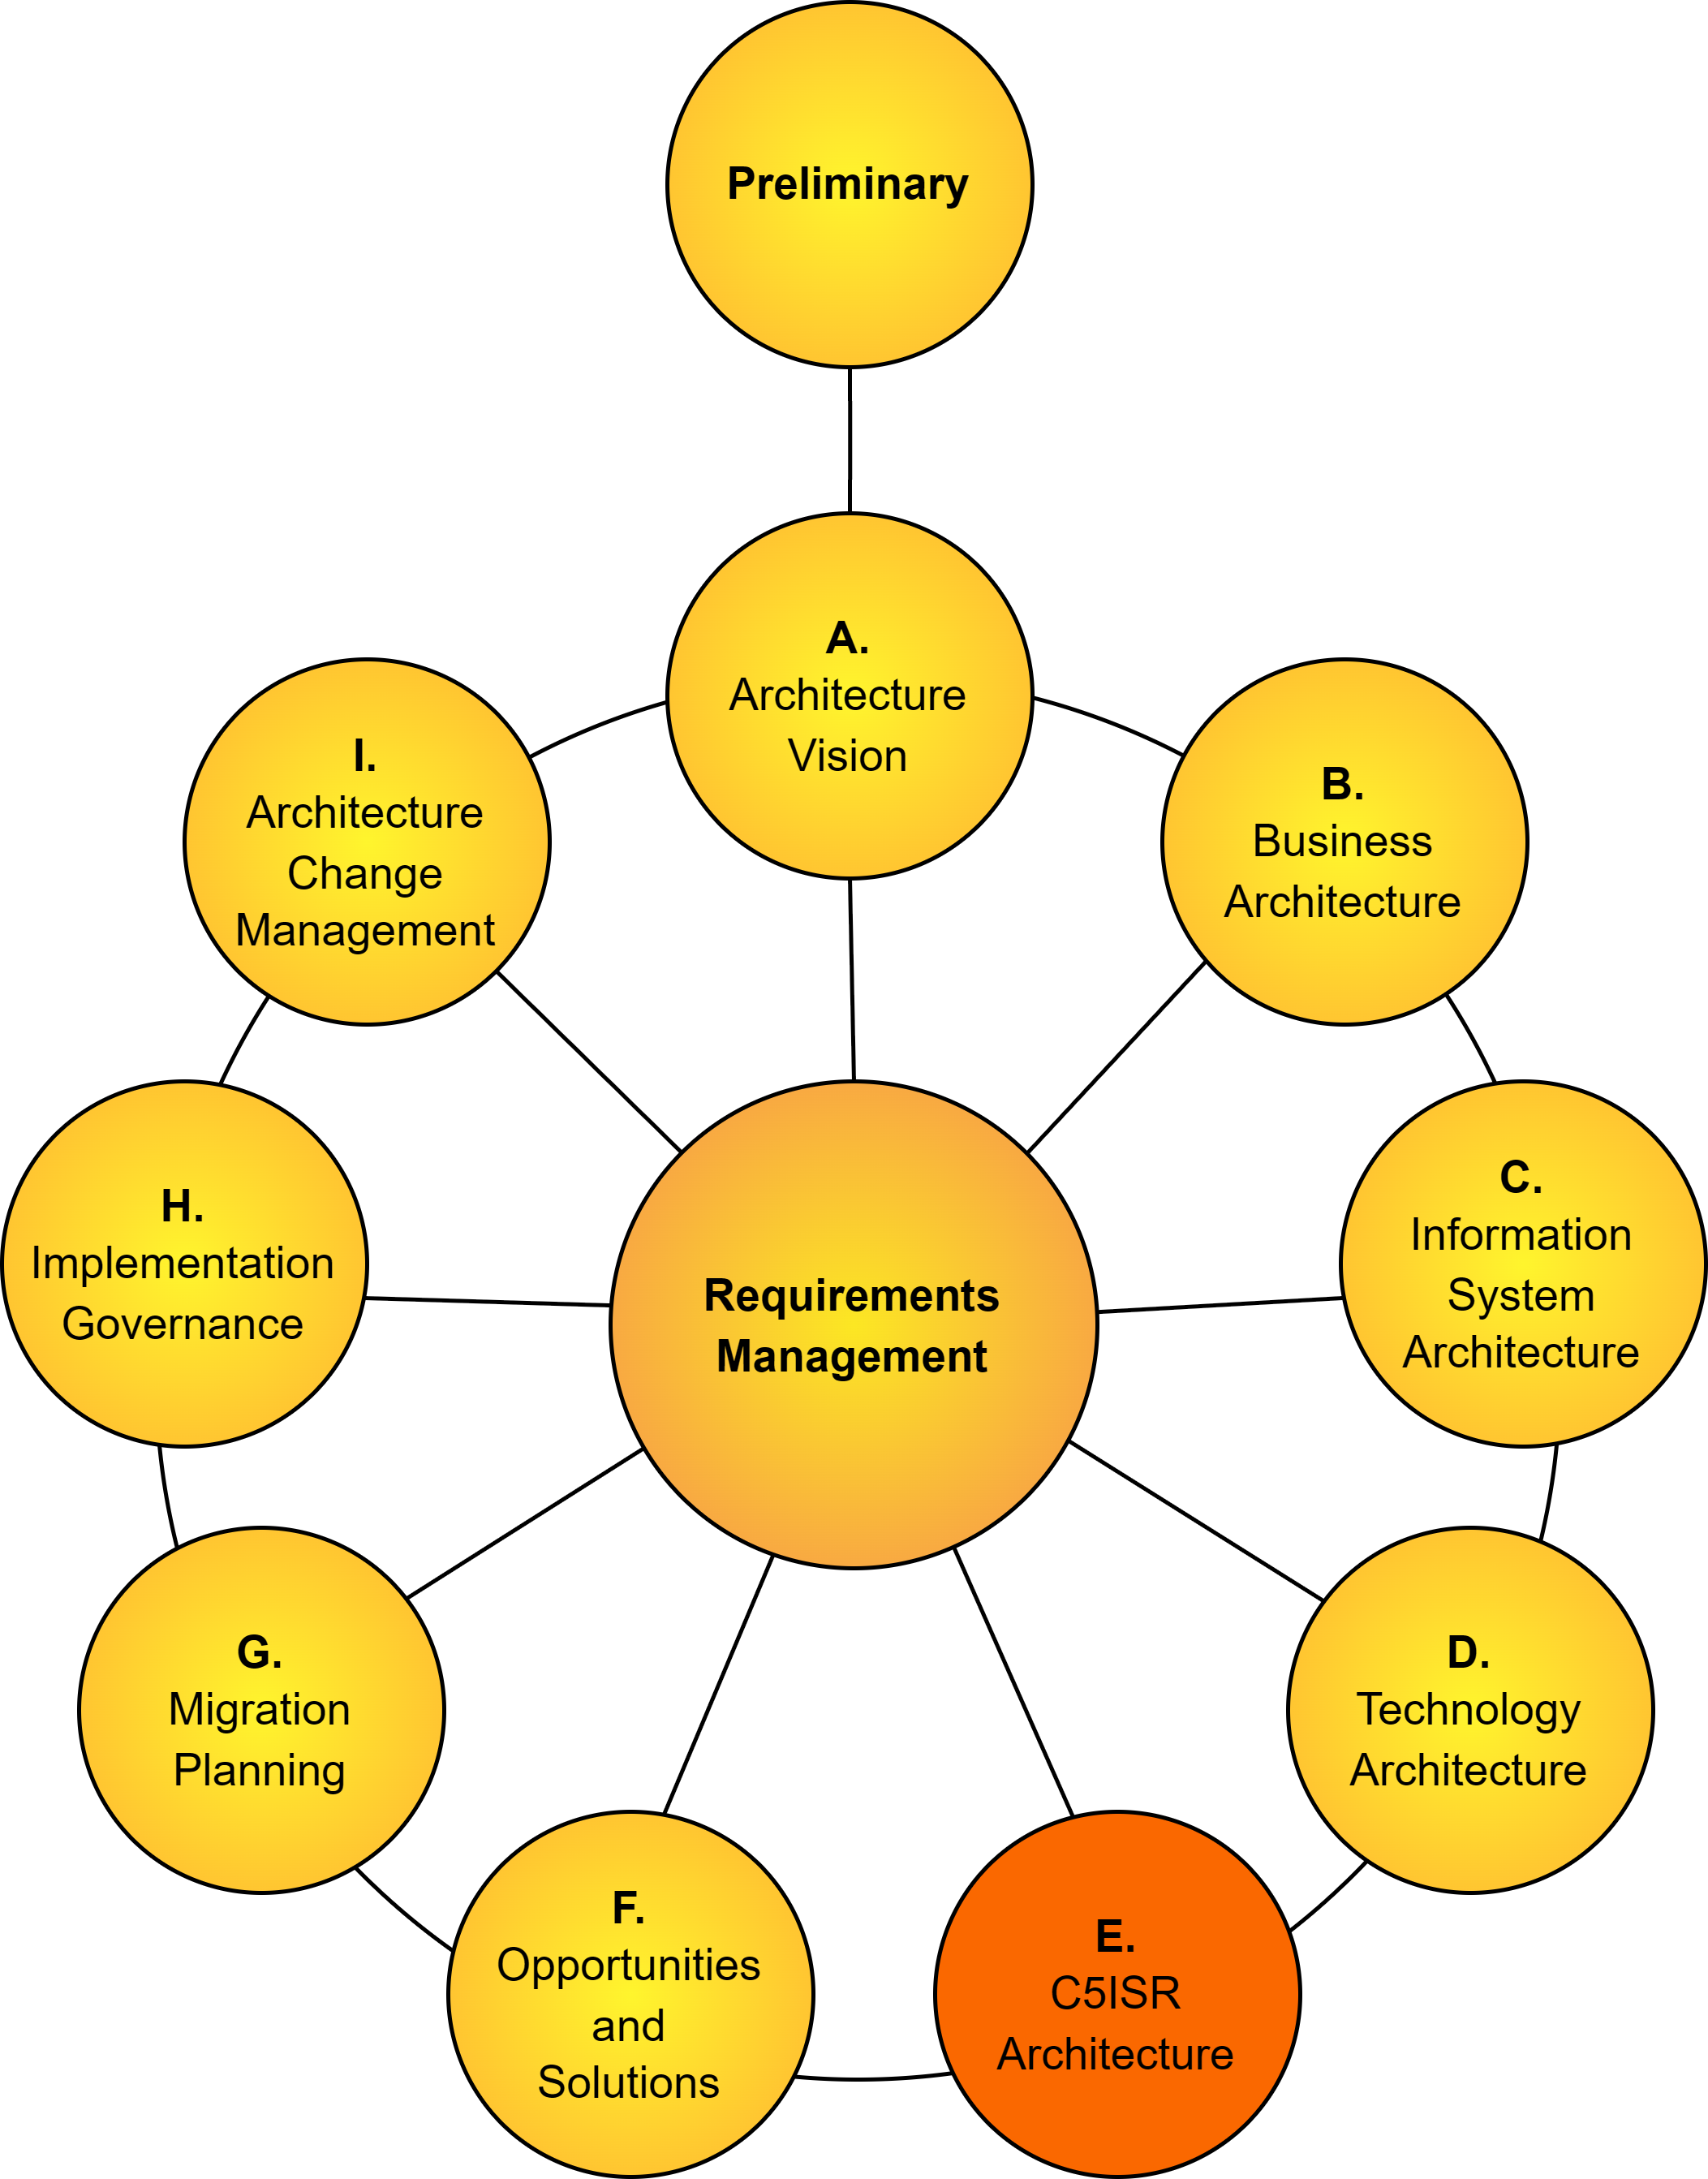
\includegraphics[width=0.9\textwidth]{images/TOGAF ADM Pertahanan indonesia.drawio.png}
\end{figure}

\subsection{Prinsip Arsitektur Pertahanan Indonesia}
\label{subsec:prinsip-arsitektur}

Prinsip arsitektur (\textit{architecture principles}) merupakan kaidah dan pedoman fundamental yang mengarahkan seluruh pengambilan keputusan dalam proses perancangan dan implementasi arsitektur. Prinsip-prinsip ini dirumuskan pada \textit{Preliminary Phase} dan menjadi acuan yang konsisten di seluruh fase, sehingga keputusan perancangan pada setiap domain arsitektur tetap terarah dan tidak saling bertentangan.

Dalam penelitian ini, prinsip arsitektur Pertahanan Indonesia diturunkan langsung dari kebutuhan \textit{framework} pada Tabel~\ref{tab:kebutuhan-framework} dan kesenjangan pada Tabel~\ref{tab:kesenjangan-framework}. Melalui prinsip inilah KF-04 dan KF-05, yang belum terpenuhi oleh TOGAF standar, dapat ditutup tanpa menambah fase baru.

Berdasarkan penurunan tersebut, dirumuskan sembilan prinsip arsitektur Pertahanan Indonesia pada Tabel~\ref{tab:prinsip-arsitektur}, lengkap dengan kebutuhan yang menjadi asal-usul setiap prinsip.

\begin{longtable}{@{}p{0.04\textwidth}p{0.24\textwidth}p{0.47\textwidth}p{0.15\textwidth}@{}}
\caption{Prinsip Arsitektur Pertahanan Indonesia}
\label{tab:prinsip-arsitektur}\\
\toprule
\textbf{No.} & \textbf{Prinsip} & \textbf{Deskripsi} & \textbf{Kebutuhan Terkait}\\
\midrule
\endfirsthead
\multicolumn{4}{c}{\tablename\ \thetable\ (lanjutan)}\\
\toprule
\textbf{No.} & \textbf{Prinsip} & \textbf{Deskripsi} & \textbf{Kebutuhan Terkait}\\
\midrule
\endhead
\bottomrule
\endfoot
1 & \textit{Interoperabilitas} & Seluruh sistem Kemhan dan ketiga angkatan harus dapat saling terintegrasi dan bertukar data secara \textit{real-time}. & KF-05\\
\addlinespace
2 & \textit{Security by Design} & Keamanan siber menjadi bagian utama arsitektur sejak tahap perencanaan, bukan sebagai tambahan di akhir. & KF-04\\
\addlinespace
3 & \textit{Data as Strategic Asset} & Data pertahanan diperlakukan sebagai aset strategis nasional untuk mendukung pengambilan keputusan. & KF-02, KF-07\\
\addlinespace
4 & \textit{Scalability \& Flexibility} & Arsitektur harus mampu berkembang mengikuti dinamika ancaman dan kemajuan teknologi di masa depan. & KF-08\\
\addlinespace
5 & \textit{Integrated Command \& Control} & Mendukung sistem komando dan pengendalian terintegrasi berbasis C5ISR. & KF-03\\
\addlinespace
6 & \textit{Availability \& Reliability} & Sistem pertahanan digital harus memiliki ketersediaan tinggi dan tahan terhadap gangguan. & KF-03, KF-06\\
\addlinespace
7 & \textit{Governance \& Compliance} & Seluruh layanan digital harus sesuai dengan regulasi pertahanan, SPBE, dan ketentuan keamanan nasional. & KF-07, KF-09\\
\addlinespace
8 & \textit{Smart Defence Oriented} & Transformasi digital harus mendukung konsep \textit{smart defence} dan operasi multi-domain. & KF-06\\
\addlinespace
9 & \textit{User-Centric Service} & Sistem dibangun untuk meningkatkan efektivitas personel dan kualitas layanan organisasi. & KF-02, KF-07\\
\end{longtable}

\subsection{TOGAF Pertahanan Indonesia}
\label{subsec:togaf-pertahanan}

TOGAF Pertahanan Indonesia merupakan hasil penyesuaian (kustomisasi) TOGAF ADM yang disesuaikan dengan kebutuhan transformasi digital sektor pertahanan. \textit{Framework} ini mempertahankan seluruh kekuatan metodologis TOGAF ADM, yaitu sifat bertahap, iteratif, dan preskriptif, dengan \textit{Requirements Management} yang tetap berada di pusat siklus sebagai pengendali konsistensi kebutuhan antarfase.

TOGAF Pertahanan Indonesia terdiri atas sepuluh fase utama, yaitu \textit{Preliminary}, \textit{Architecture Vision}, \textit{Business Architecture}, \textit{Information Systems Architecture}, \textit{Technology Architecture}, \textit{C5ISR Architecture}, \textit{Opportunities \& Solutions}, \textit{Migration Planning}, \textit{Implementation Governance}, dan \textit{Architecture Change Management}.

Kesepuluh fase tersebut dapat dipandang sebagai tiga kelompok yang berurutan. Kelompok pertama adalah fase penetapan arah dan fondasi, yang mencakup \textit{Preliminary} dan \textit{Architecture Vision}. Pada kelompok inilah muatan pertahanan ditanamkan paling awal, yaitu melalui penetapan doktrin dan strategi pertahanan nasional sebagai masukan serta penetapan prinsip arsitektur.

Kelompok kedua adalah fase pengembangan domain arsitektur, yang mencakup \textit{Business Architecture}, \textit{Information Systems Architecture}, \textit{Technology Architecture}, dan \textit{C5ISR Architecture}. Tiga fase pertama merupakan bagian standar TOGAF yang dipertahankan tanpa pengurangan, sedangkan Fase \textit{C5ISR Architecture} merupakan fase baru yang menjadi pembeda utama \textit{framework} ini dari TOGAF standar.

Kelompok ketiga adalah fase realisasi dan keberlanjutan, yang mencakup \textit{Opportunities \& Solutions}, \textit{Migration Planning}, \textit{Implementation Governance}, dan \textit{Architecture Change Management}. Keempat fase ini dipertahankan sebagaimana adanya pada TOGAF ADM standar karena telah memadai untuk menjamin bahwa arsitektur yang dirancang dapat diwujudkan, dikendalikan, dan dipelihara relevansinya secara berkelanjutan.

Setiap fase diuraikan dalam format yang seragam, yaitu masukan (\textit{input}), langkah utama (\textit{step}), dan keluaran (\textit{output}), sehingga setiap fase dapat langsung dijadikan panduan pelaksanaan.

\subsubsection{Fase \textit{Preliminary}}

Fase \textit{Preliminary} merupakan fase persiapan yang menetapkan fondasi bagi keseluruhan pengembangan arsitektur. Pada fase ini ditetapkan ruang lingkup transformasi digital pertahanan, prinsip-prinsip arsitektur, struktur tata kelola arsitektur, serta penilaian kesiapan organisasi. Fase ini juga memastikan keterkaitan arsitektur dengan kerangka regulasi nasional dan sektor pertahanan, sehingga arsitektur yang dihasilkan selaras dengan kebijakan yang berlaku.

\begin{figure}[htbp]
\centering
\caption{Kedudukan Fase \textit{Preliminary} pada Siklus TOGAF Pertahanan Indonesia}
\label{fig:fase-preliminary}
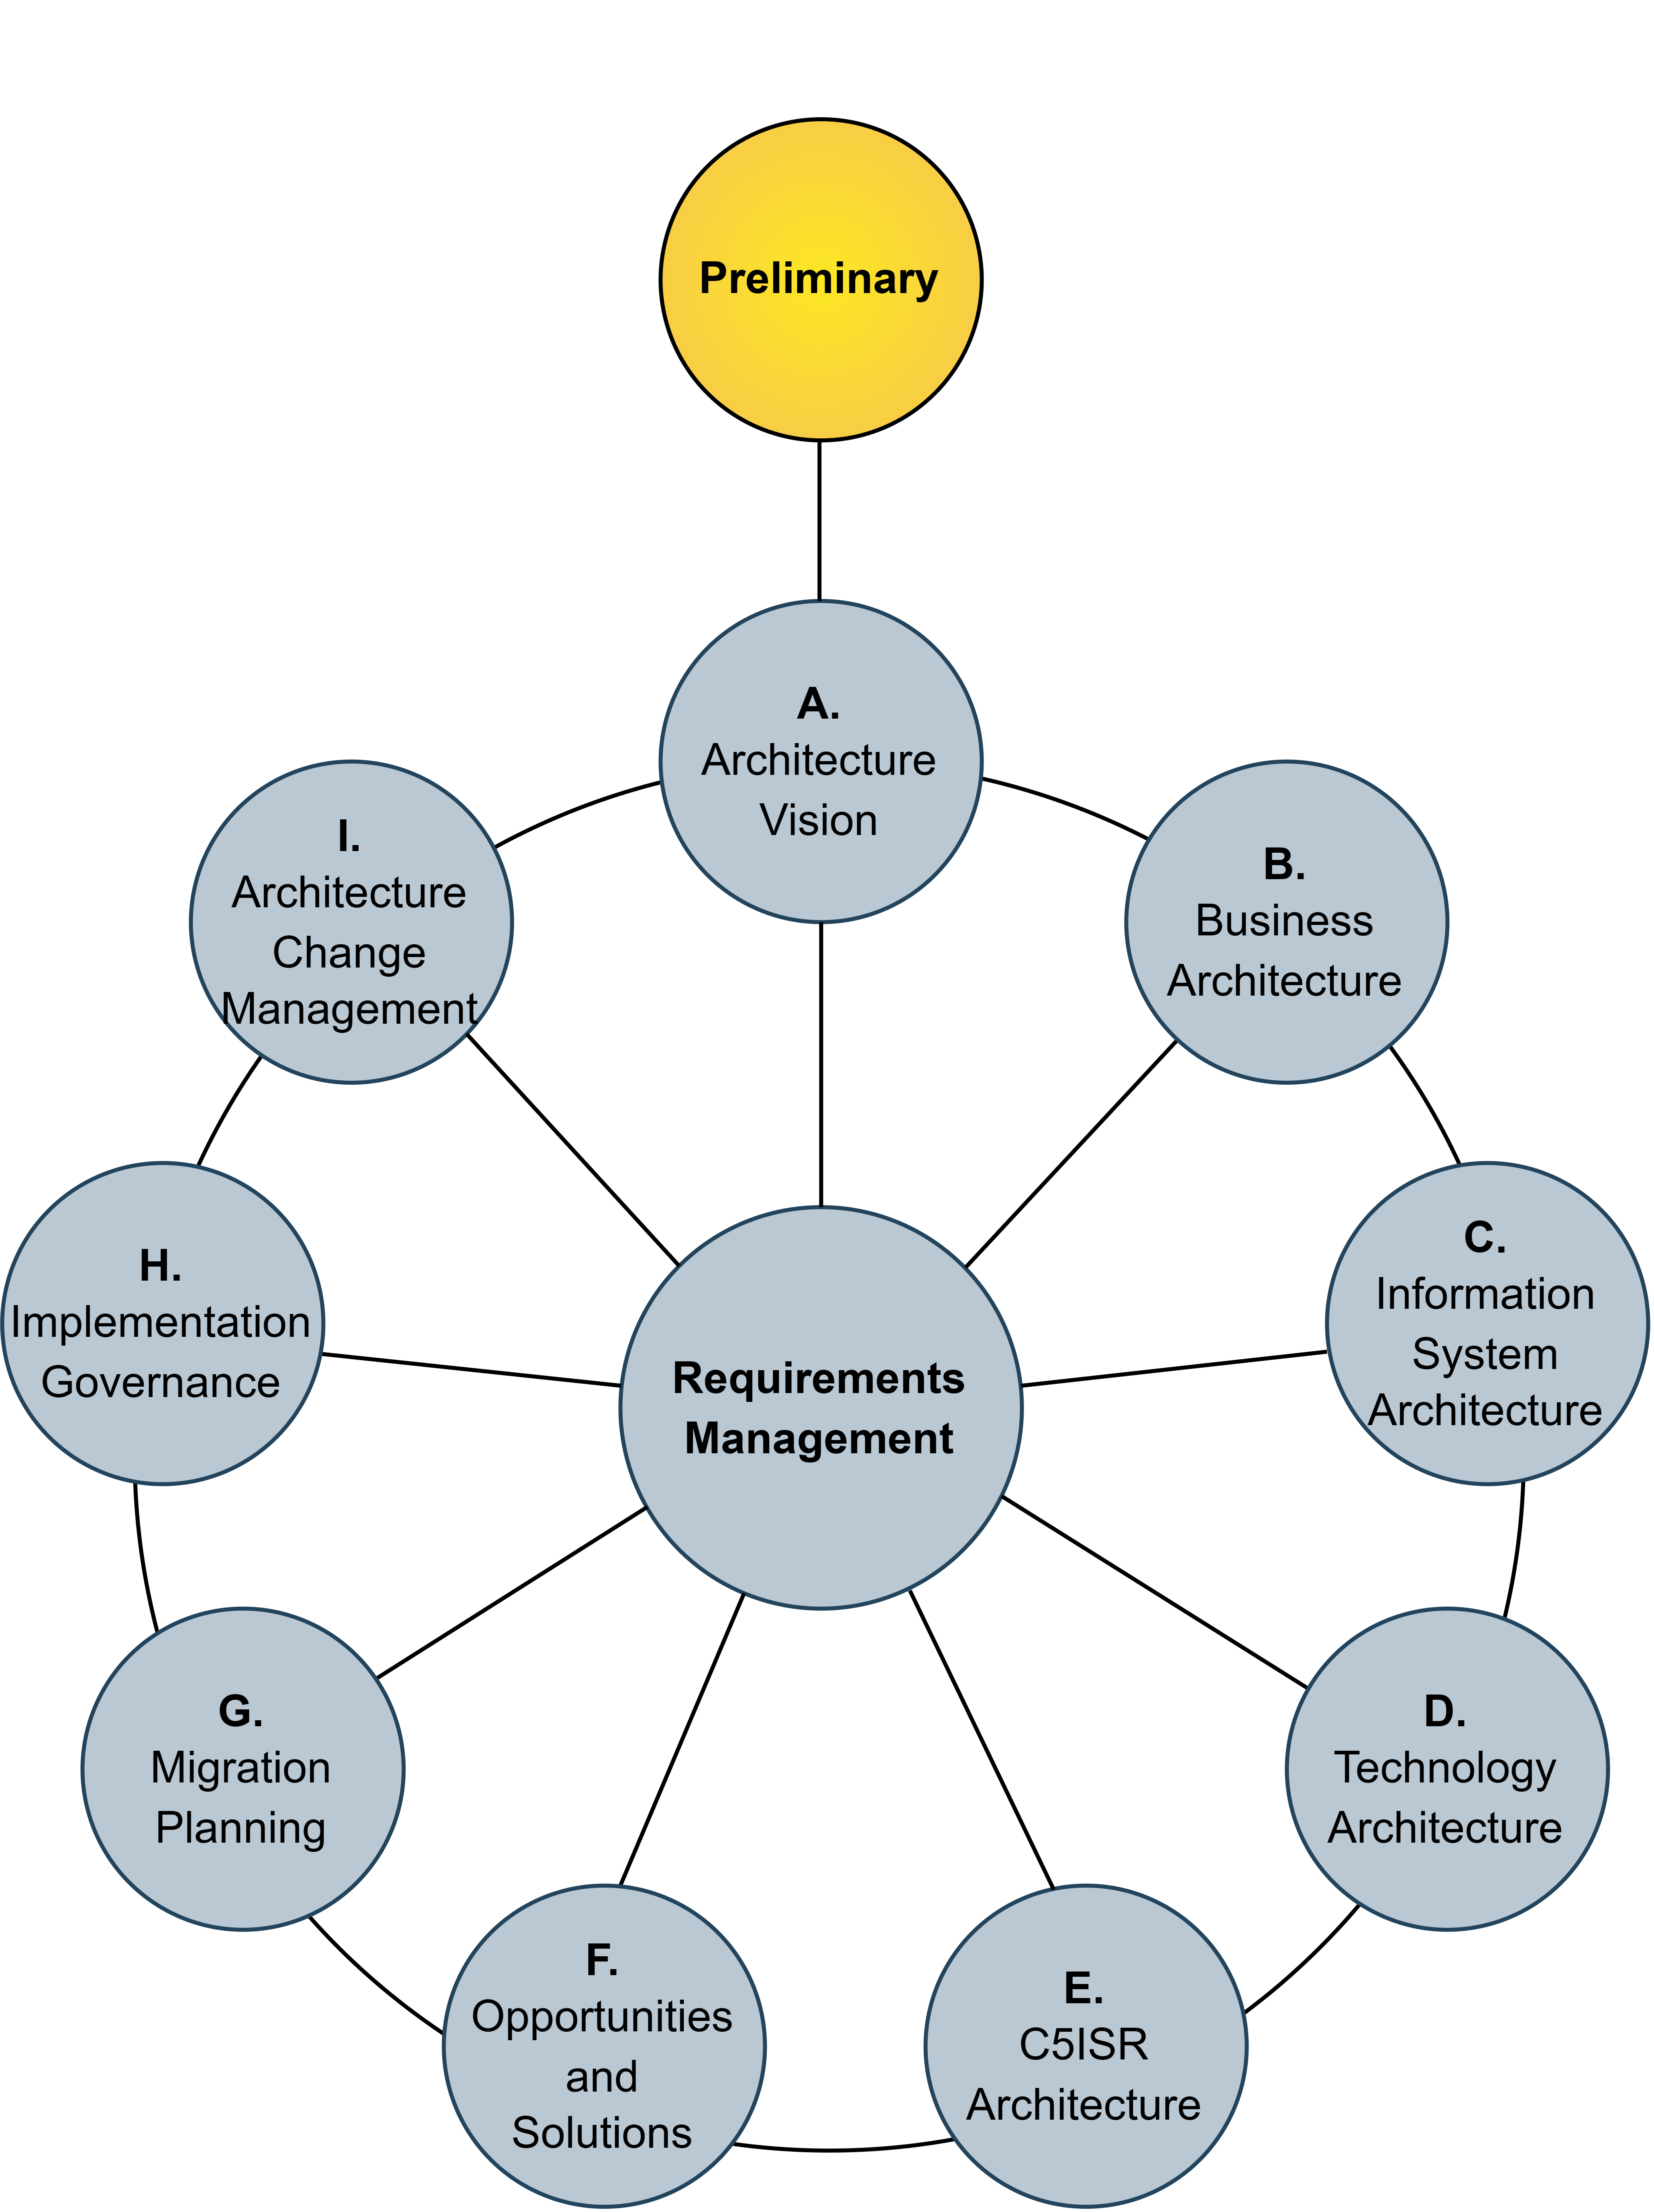
\includegraphics[width=0.42\textwidth]{images/Preliminary.drawio.png}
\end{figure}

Gambar~\ref{fig:fase-preliminary} menempatkan fase \textit{Preliminary} pada puncak siklus, terpisah dari kesembilan fase lain yang mengelilingi \textit{Requirements Management}. Kedudukan ini menegaskan sifatnya sebagai fase persiapan yang dijalankan satu kali di awal untuk membentuk fondasi seluruh siklus, bukan bagian dari perulangan pengembangan arsitektur. Pada fase inilah kesiapan organisasi dinilai, tim arsitektur dibentuk, prinsip arsitektur ditetapkan, dan kerangka TOGAF disesuaikan menjadi TOGAF Pertahanan Indonesia. Rincian \textit{input}, \textit{step} dan \textit{output} yang membentuk fase tersebut terdapat pada Tabel~\ref{tab:fase-preliminary}.

\begin{longtable}{@{}p{0.31\textwidth}p{0.31\textwidth}p{0.31\textwidth}@{}}
\caption{\textit{Input}, \textit{Step}, dan \textit{Output} Fase \textit{Preliminary}}
\label{tab:fase-preliminary}\\
\toprule
\textbf{\textit{INPUT}} & \textbf{\textit{STEP}} & \textbf{\textit{OUTPUT}}\\
\midrule
\endfirsthead
\multicolumn{3}{c}{\tablename\ \thetable\ (lanjutan)}\\
\toprule
\textbf{\textit{INPUT}} & \textbf{\textit{STEP}} & \textbf{\textit{OUTPUT}}\\
\midrule
\endhead
\bottomrule
\endfoot
\raggedright
1. \textit{TOGAF reference material} dan \textit{TOGAF Library}\newline
2. Kerangka arsitektur pertahanan sebagai rujukan\newline
3. Doktrin dan strategi pertahanan nasional\newline
4. Rencana strategis transformasi digital Kemhan\newline
5. Standar industri pertahanan\newline
6. Kerangka regulasi dan tata kelola, mencakup SPBE dan Satu Data Indonesia\newline
7. Informasi pemangku kepentingan dan struktur organisasi\newline
8. Kapabilitas arsitektur yang telah dimiliki organisasi\newline
9. Perjanjian kemitraan dan kontrak kerja sama industri pertahanan
&
\raggedright
1. Menentukan ruang lingkup organisasi yang terdampak transformasi digital pertahanan\newline
2. Mengonfirmasi kerangka tata kelola dan kerangka pendukung\newline
3. Mendefinisikan dan membentuk tim serta organisasi \textit{Enterprise Architecture} pertahanan\newline
4. Mengidentifikasi dan menetapkan prinsip arsitektur pertahanan\newline
5. Melakukan penyesuaian (\textit{tailoring}) kerangka TOGAF menjadi TOGAF Pertahanan Indonesia\newline
6. Mengidentifikasi keterkaitan arsitektur dengan regulasi nasional dan sektor pertahanan\newline
7. Menetapkan definisi \textit{smart defence} dan prinsip interoperabilitas sebagai acuan bersama
&
\raggedright
1. Model organisasi untuk arsitektur \textit{enterprise} (\textit{organizational model})\newline
2. Kerangka arsitektur hasil penyesuaian, yaitu TOGAF Pertahanan Indonesia\newline
3. \textit{Architecture Repository} awal yang telah diisi muatan kerangka\newline
4. Prinsip arsitektur pertahanan\newline
5. Kerangka tata kelola arsitektur (\textit{architecture governance framework})\newline
6. Dokumen ruang lingkup dan keterkaitan regulasi\newline
7. \textit{Request for Architecture Work}\newline
8. Arsitektur kapabilitas \textit{Enterprise Architecture}\arraybackslash\\
\end{longtable}

Fase \textit{Preliminary} TOGAF Pertahanan Indonesia menghadirkan konteks pertahanan sejak titik paling awal. Fase ini menerima \textit{input} doktrin dan strategi pertahanan nasional, standar industri pertahanan, serta kerangka regulasi dan tata kelola yang mencakup SPBE dan Satu Data Indonesia. Ketiga kelompok \textit{input} ini memastikan bahwa arsitektur yang akan dibentuk selaras dengan karakteristik organisasi pertahanan dan berada sesuai dengan hukum yang berlaku.

Langkah-langkah fase ini bergerak dari penetapan ruang lingkup organisasi yang terdampak, pembentukan tim arsitektur, hingga penetapan prinsip arsitektur pertahanan. Langkah yang paling menentukan adalah penyesuaian kerangka TOGAF ADM menjadi TOGAF Pertahanan Indonesia, karena pada langkah inilah struktur sepuluh fase, prinsip pertahanan, dan penempatan fase C5ISR ditetapkan.

\textit{Output} dari fase ini merupakan perangkat kerja bagi seluruh siklus. Model organisasi arsitektur, kerangka tata kelola arsitektur, dan prinsip arsitektur pertahanan menjadi acuan pengendalian mutu pada setiap fase.

\subsubsection{Fase \textit{Architecture Vision}}

Pada fase \textit{Architecture Vision} dilakukan perumusan visi, misi, dan tujuan strategis arsitektur transformasi digital pertahanan, serta identifikasi pemangku kepentingan utama. Fase ini memberikan gambaran tingkat tinggi mengenai kondisi target (\textit{to-be}) yang ingin dicapai dan menjadi acuan arah bagi seluruh fase berikutnya.

\begin{figure}[htbp]
\centering
\caption{Kedudukan Fase \textit{Architecture Vision} pada Siklus TOGAF Pertahanan Indonesia}
\label{fig:fase-vision}
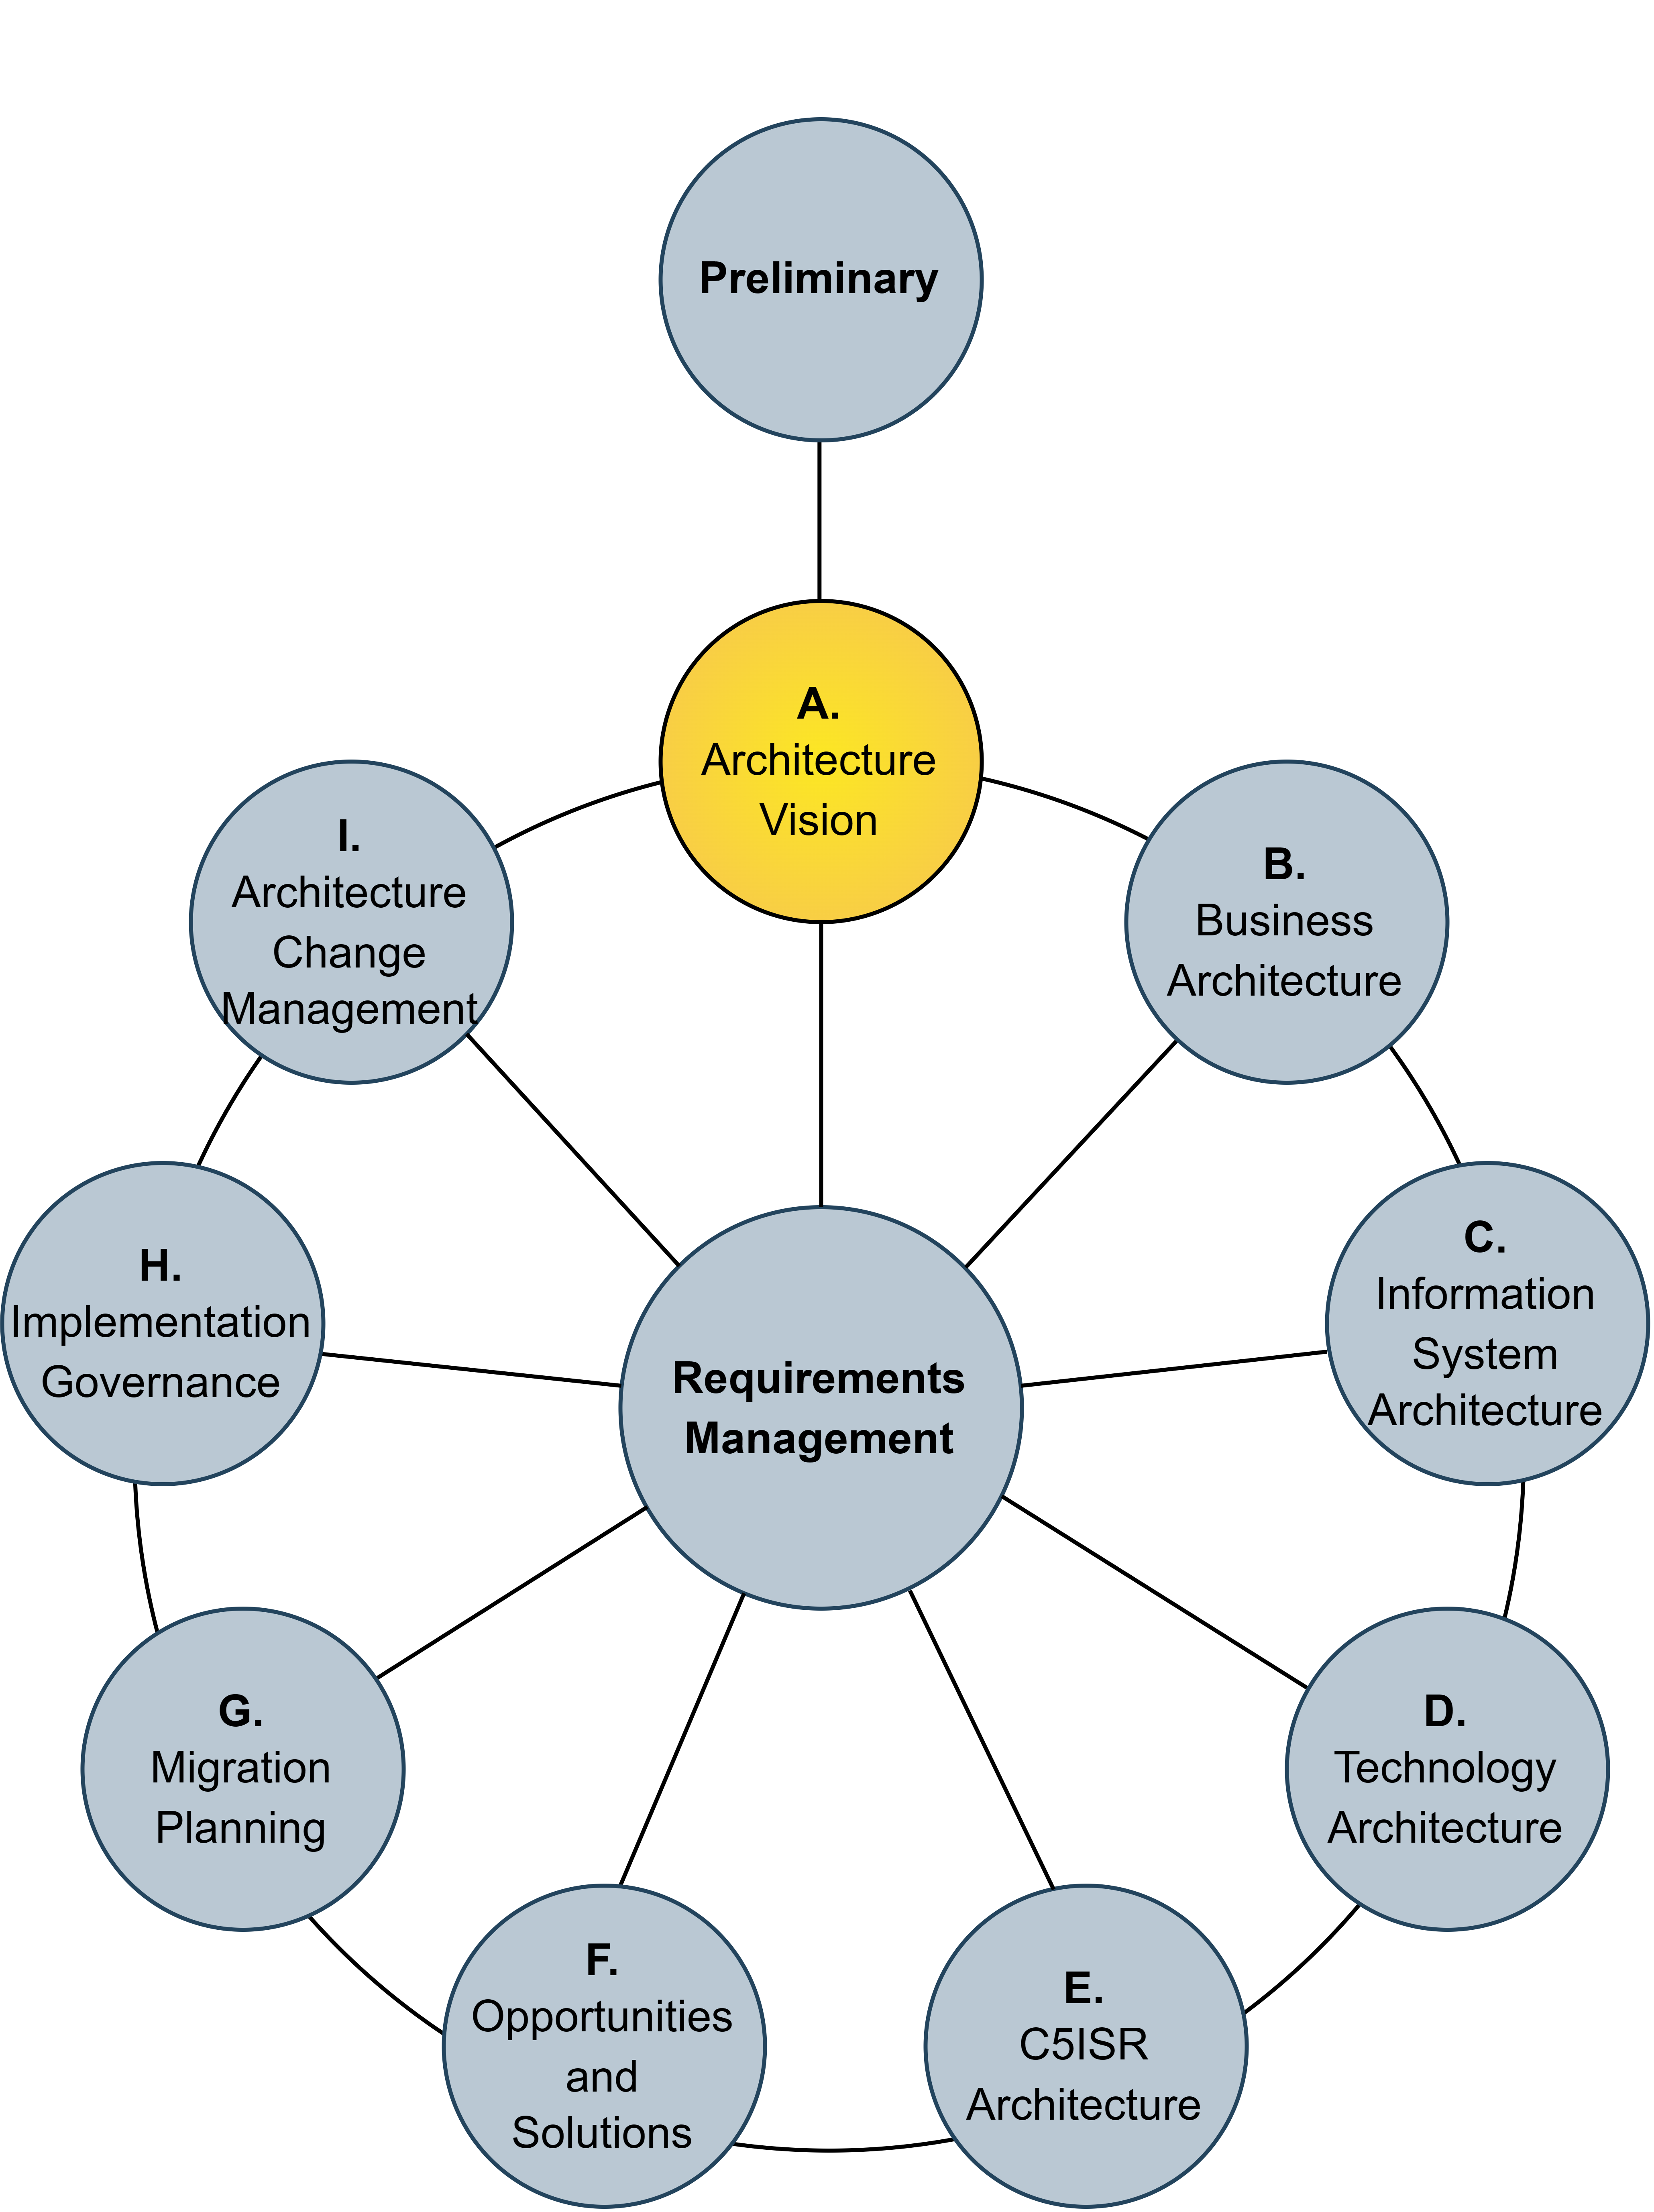
\includegraphics[width=0.42\textwidth]{images/Architecture Vision.drawio.png}
\end{figure}

Gambar~\ref{fig:fase-vision} menunjukkan fase \textit{Architecture Vision} sebagai fase pertama yang terhubung langsung dengan \textit{Requirements Management} di pusat siklus. Posisi ini menandai peralihan dari persiapan menuju pengembangan, yaitu titik ketika kebutuhan pemangku kepentingan mulai dikumpulkan dan diterjemahkan menjadi arah arsitektur. \textit{Input}, \textit{step} dan \textit{output} yang menghasilkan arah tersebut diuraikan pada Tabel~\ref{tab:fase-vision}.

\begin{longtable}{@{}p{0.31\textwidth}p{0.31\textwidth}p{0.31\textwidth}@{}}
\caption{\textit{Input}, \textit{Step}, dan \textit{Output} Fase \textit{Architecture Vision}}
\label{tab:fase-vision}\\
\toprule
\textbf{INPUT} & \textbf{STEP} & \textbf{OUTPUT}\\
\midrule
\endfirsthead
\multicolumn{3}{c}{\tablename\ \thetable\ (lanjutan)}\\
\toprule
\textbf{INPUT} & \textbf{STEP} & \textbf{OUTPUT}\\
\midrule
\endhead
\bottomrule
\endfoot
\raggedright
1. \textit{Architecture reference materials}\newline
2. \textit{Request for Architecture Work}\newline
3. Prinsip, sasaran, dan pendorong organisasi pertahanan\newline
4. Model organisasi untuk arsitektur \textit{enterprise}\newline
5. TOGAF Pertahanan Indonesia hasil penyesuaian\newline
6. \textit{Architecture Repository} yang telah terisi\newline
7. Kerangka regulasi nasional serta doktrin dan strategi pertahanan
&
\raggedright
1. Menetapkan proyek arsitektur\newline
2. Mengidentifikasi pemangku kepentingan, kepedulian (\textit{concern}), dan kebutuhan organisasi\newline
3. Mengonfirmasi dan menguraikan sasaran, pendorong, serta kendala organisasi pertahanan\newline
4. Mengevaluasi kapabilitas organisasi\newline
5. Menilai kesiapan organisasi terhadap transformasi\newline
6. Menetapkan ruang lingkup arsitektur\newline
7. Mengonfirmasi dan menguraikan prinsip arsitektur pertahanan\newline
8. Menyusun visi dan misi arsitektur pertahanan digital\newline
9. Menetapkan proposisi nilai manfaat arsitektur target dan indikator kinerja utama\newline
10. Mengidentifikasi risiko transformasi dan tindakan mitigasinya\newline
11. Menyusun \textit{statement of architecture work} dan memperoleh persetujuan
&
\raggedright
1. \textit{Statement of Architecture Work} yang disetujui\newline
2. Pernyataan yang telah diperbarui mengenai prinsip, sasaran, dan pendorong organisasi\newline
3. Prinsip arsitektur pertahanan yang telah dikonfirmasi\newline
4. Hasil penilaian kapabilitas (\textit{capability assessment})\newline
5. TOGAF Pertahanan Indonesia yang telah disesuaikan\newline
6. Dokumen \textit{Architecture Vision} berisi visi dan misi pertahanan digital\newline
7. Peta pemangku kepentingan (\textit{stakeholder map})\newline
8. Tujuan strategis arsitektur pertahanan\newline
9. Rencana komunikasi (\textit{communications plan})\newline
10. Tambahan \textit{file} yang mengisi \textit{Architecture Repository}\arraybackslash\\
\end{longtable}

\textit{Input} fase ini bertumpu pada \textit{output} fase \textit{Preliminary}, ditambah satu masukan khas berupa kerangka regulasi nasional serta doktrin dan strategi pertahanan. \textit{Input} ini memastikan bahwa visi arsitektur yang dirumuskan tidak menyimpang dari arah kebijakan pertahanan nasional.

Rangkaian langkah-langkah fase ini menuntun penyusunan visi secara sistematis, mulai dari penetapan proyek arsitektur, identifikasi pemangku kepentingan beserta kepeduliannya, penilaian kesiapan organisasi, hingga penyusunan visi dan misi pertahanan digital.

\textit{Output} fase ini menetapkan arah yang mengikat fase-fase berikutnya. Dokumen \textit{Architecture Vision}, prinsip arsitektur yang telah dikonfirmasi, peta pemangku kepentingan, dan tujuan strategis arsitektur menjadi rujukan bersama, sedangkan rencana komunikasi mengatur penyampaian kemajuan kepada tiap kelompok pemangku kepentingan yang berjenjang di lingkungan Kemhan dan TNI.

\subsubsection{Fase \textit{Business Architecture}}

Pada fase \textit{Business Architecture} dilakukan perancangan model proses bisnis, kapabilitas, dan organisasi pertahanan yang efektif untuk mendukung komando dan kendali, integrasi data, serta kolaborasi lintas satuan.

\begin{figure}[htbp]
\centering
\caption{Kedudukan Fase \textit{Business Architecture} pada Siklus TOGAF Pertahanan Indonesia}
\label{fig:fase-business}
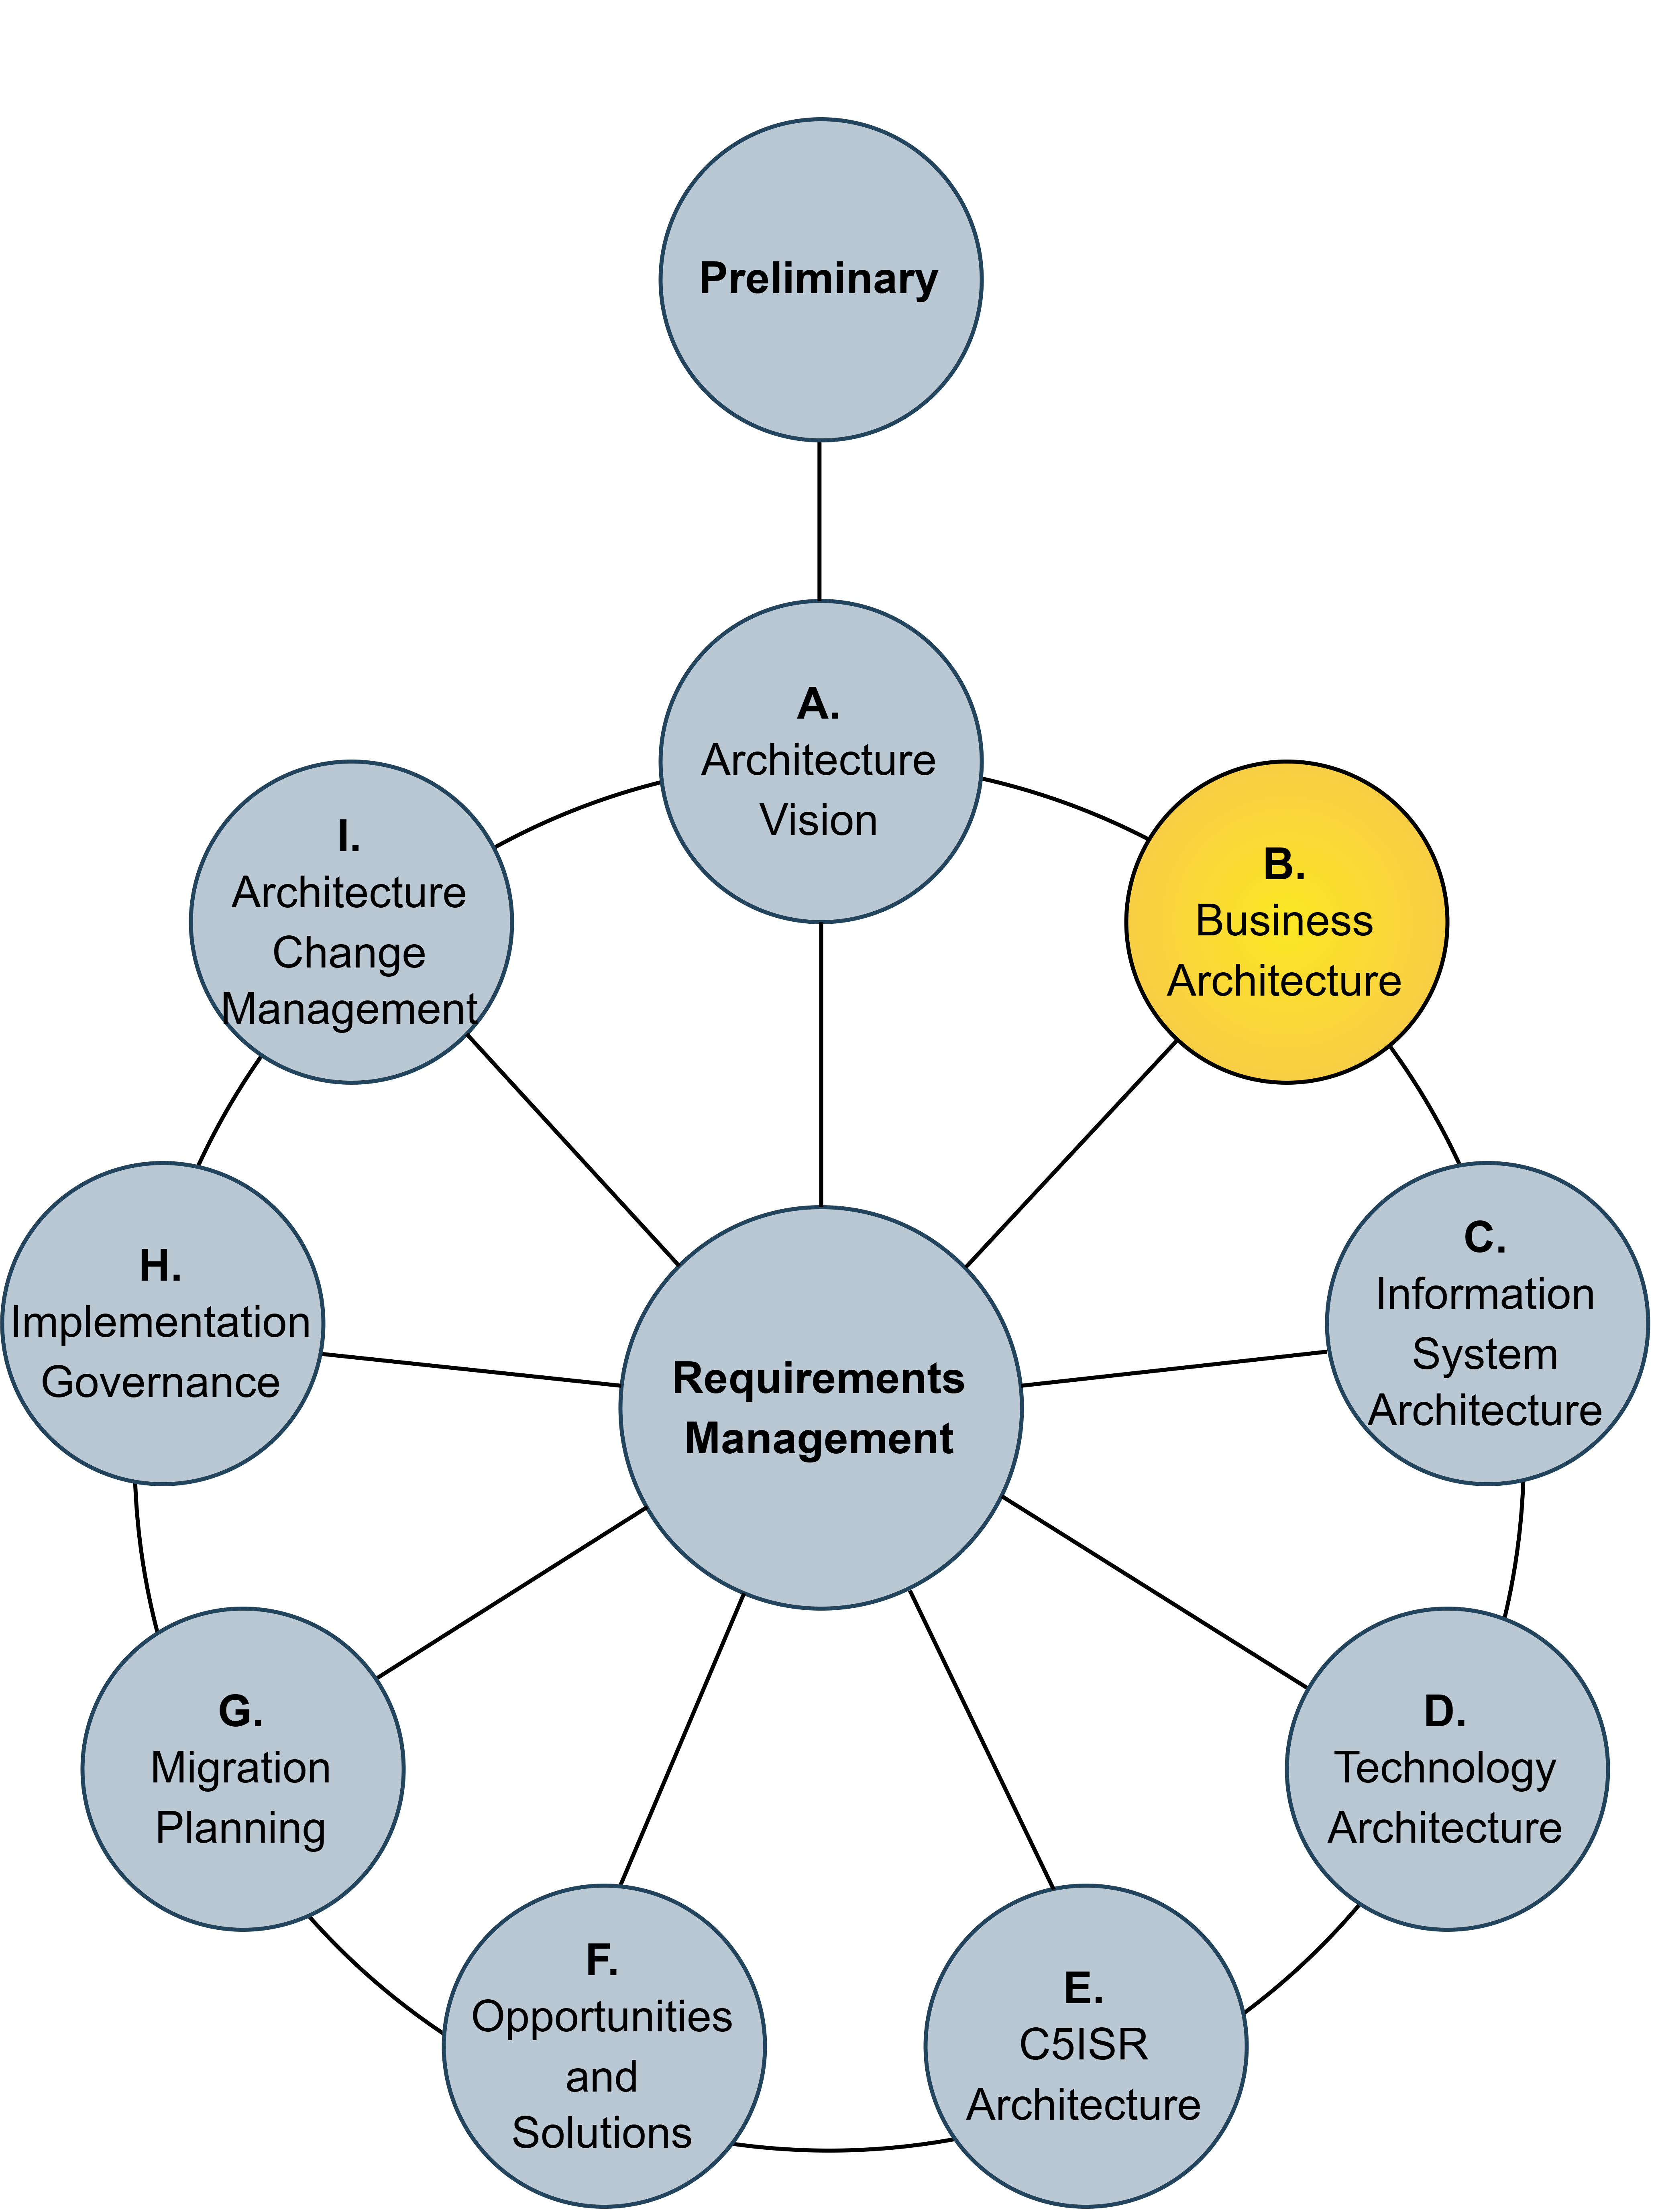
\includegraphics[width=0.42\textwidth]{images/Business Architecture.drawio.png}
\end{figure}

Gambar~\ref{fig:fase-business} menempatkan fase \textit{Business Architecture} sebagai fase pertama dari kelompok pengembangan domain arsitektur. Sebagai fase yang menerjemahkan visi menjadi rancangan organisasi yang konkret, \textit{Business Architecture} menjadi pijakan bagi perancangan arsitektur data, aplikasi, teknologi, dan C5ISR pada fase-fase sesudahnya. Uraian \textit{input}, \textit{step}, dan \textit{output} dapat dilihat pada Tabel~\ref{tab:fase-business}.

\begin{longtable}{@{}p{0.31\textwidth}p{0.31\textwidth}p{0.31\textwidth}@{}}
\caption{\textit{Input}, \textit{Step}, dan \textit{Output} Fase \textit{Business Architecture}}
\label{tab:fase-business}\\
\toprule
\textbf{INPUT} & \textbf{STEP} & \textbf{OUTPUT}\\
\midrule
\endfirsthead
\multicolumn{3}{c}{\tablename\ \thetable\ (lanjutan)}\\
\toprule
\textbf{INPUT} & \textbf{STEP} & \textbf{OUTPUT}\\
\midrule
\endhead
\bottomrule
\endfoot
\raggedright
1. \textit{Architecture reference materials}\newline
2. \textit{Request for Architecture Work}\newline
3. Prinsip, sasaran, dan pendorong organisasi pertahanan\newline
4. Hasil penilaian kapabilitas dan rencana komunikasi\newline
5. Model organisasi untuk arsitektur \textit{enterprise}\newline
6. TOGAF Pertahanan Indonesia\newline
7. \textit{Statement of Architecture Work} yang disetujui\newline
8. Prinsip arsitektur pertahanan\newline
9. \textit{Enterprise Continuum} dan \textit{Architecture Repository}\newline
10. Dokumen \textit{Architecture Vision}\newline
11. Draf \textit{Architecture Definition Document}\newline
12. Struktur organisasi dan proses bisnis saat ini Kemhan dan TNI\newline
13. Strategi pertahanan dan transformasi digital
&
\raggedright
1. Memilih model rujukan, sudut pandang (\textit{viewpoint}), dan perangkat pemodelan\newline
2. Menyusun deskripsi arsitektur bisnis \textit{baseline}\newline
3. Memodelkan proses bisnis inti dan proses bisnis pendukung pertahanan\newline
4. Menyusun peta kapabilitas (\textit{business capability map}) dan \textit{value stream} pertahanan\newline
5. Menyusun deskripsi arsitektur bisnis target\newline
6. Melakukan analisis kesenjangan (\textit{as-is vs to-be})\newline
7. Menetapkan komponen kandidat \textit{roadmap}\newline
8. Menyelesaikan dampak lintas lanskap arsitektur\newline
9. Melaksanakan tinjauan formal pemangku kepentingan\newline
10. Memfinalkan arsitektur bisnis\newline
11. Menyusun atau memutakhirkan \textit{Architecture Definition Document}
&
\raggedright
1. Versi yang diperhalus dan dimutakhirkan dari keluaran fase \textit{Architecture Vision}\newline
2. Draf \textit{Architecture Definition Document}\newline
3. Draf \textit{Architecture Requirements Specification}\newline
4. Komponen arsitektur bisnis pada \textit{roadmap} arsitektur\newline
5. Peta kapabilitas pertahanan (\textit{business capability map})\newline
6. \textit{Value stream} pertahanan\newline
7. Model tata kelola dan komando\newline
8. Model operasi dan interoperabilitas lintas matra\arraybackslash\\
\end{longtable}

\textit{Input} fase ini mencakup arahan strategis dari fase \textit{Architecture Vision} serta gambaran struktur organisasi dan proses bisnis saat ini di lingkungan Kemhan dan TNI. Kombinasi keduanya pada fase ini menghasilkan perbandingan kondisi saat ini (\textit{as-is}) dengan kondisi yang dituju (\textit{target}), sehingga rancangan yang dihasilkan berangkat dari keadaan nyata organisasi pertahanan.

Langkah-langkah fase ini menegaskan pendekatan berbasis kapabilitas. Pemodelan proses bisnis inti dan pendukung, penyusunan peta kapabilitas, dan penyusunan \textit{value stream} pertahanan menempatkan kapabilitas sebagai analisis utama. Setelah arsitektur bisnis target disusun, analisis kesenjangan mengidentifikasi selisih antara kondisi saat ini dan kondisi target yang harus ditutup.

\textit{Output} fase ini menyediakan pijakan organisasional bagi fase berikutnya. Peta kapabilitas dan \textit{value stream} pertahanan menjadi acuan penurunan kebutuhan data dan aplikasi, sedangkan model tata kelola dan komando serta model operasi dan interoperabilitas lintas matra secara khusus menyiapkan landasan bagi perancangan arsitektur komando dan kendali pada fase C5ISR. Dengan demikian, arsitektur C5ISR tidak dirancang terlepas dari struktur organisasi yang menjalankannya.

\subsubsection{Fase \textit{Information Systems Architecture}}

Fase \textit{Information Systems Architecture} dilakukan untuk menentukan arsitektur sistem informasi yang mendukung proses bisnis pertahanan. Fase ini mencakup dua sub-domain, yaitu arsitektur data (\textit{data architecture}) dan arsitektur aplikasi (\textit{application architecture}).

Pada TOGAF Pertahanan Indonesia, kedua sub-domain dikerjakan secara berurutan dengan arsitektur data didahulukan. Karena permasalahan utama ekosistem digital pertahanan terletak pada data yang terkotak-kotak antarsatuan, sehingga penetapan definisi, klasifikasi, dan kepemilikan data harus lebih dahulu diselesaikan sebelum portofolio aplikasi dirancang.

\paragraph{\textit{Data Architecture}}\mbox{}\\
Arsitektur data merancang struktur definisi, klasifikasi, dan tata kelola kepemilikan data pertahanan. Perancangan arsitektur data berpedoman pada prinsip \textit{Data as Strategic Asset}, serta pada ketentuan Satu Data Indonesia dan ketentuan klasifikasi informasi pertahanan. Kedudukan sub-domain ini dalam siklus TOGAF Pertahanan Indonesia ditunjukkan pada Gambar~\ref{fig:fase-data}.

\begin{figure}[htbp]
\centering
\caption{Kedudukan Sub-domain \textit{Data Architecture} pada Siklus TOGAF Pertahanan Indonesia}
\label{fig:fase-data}
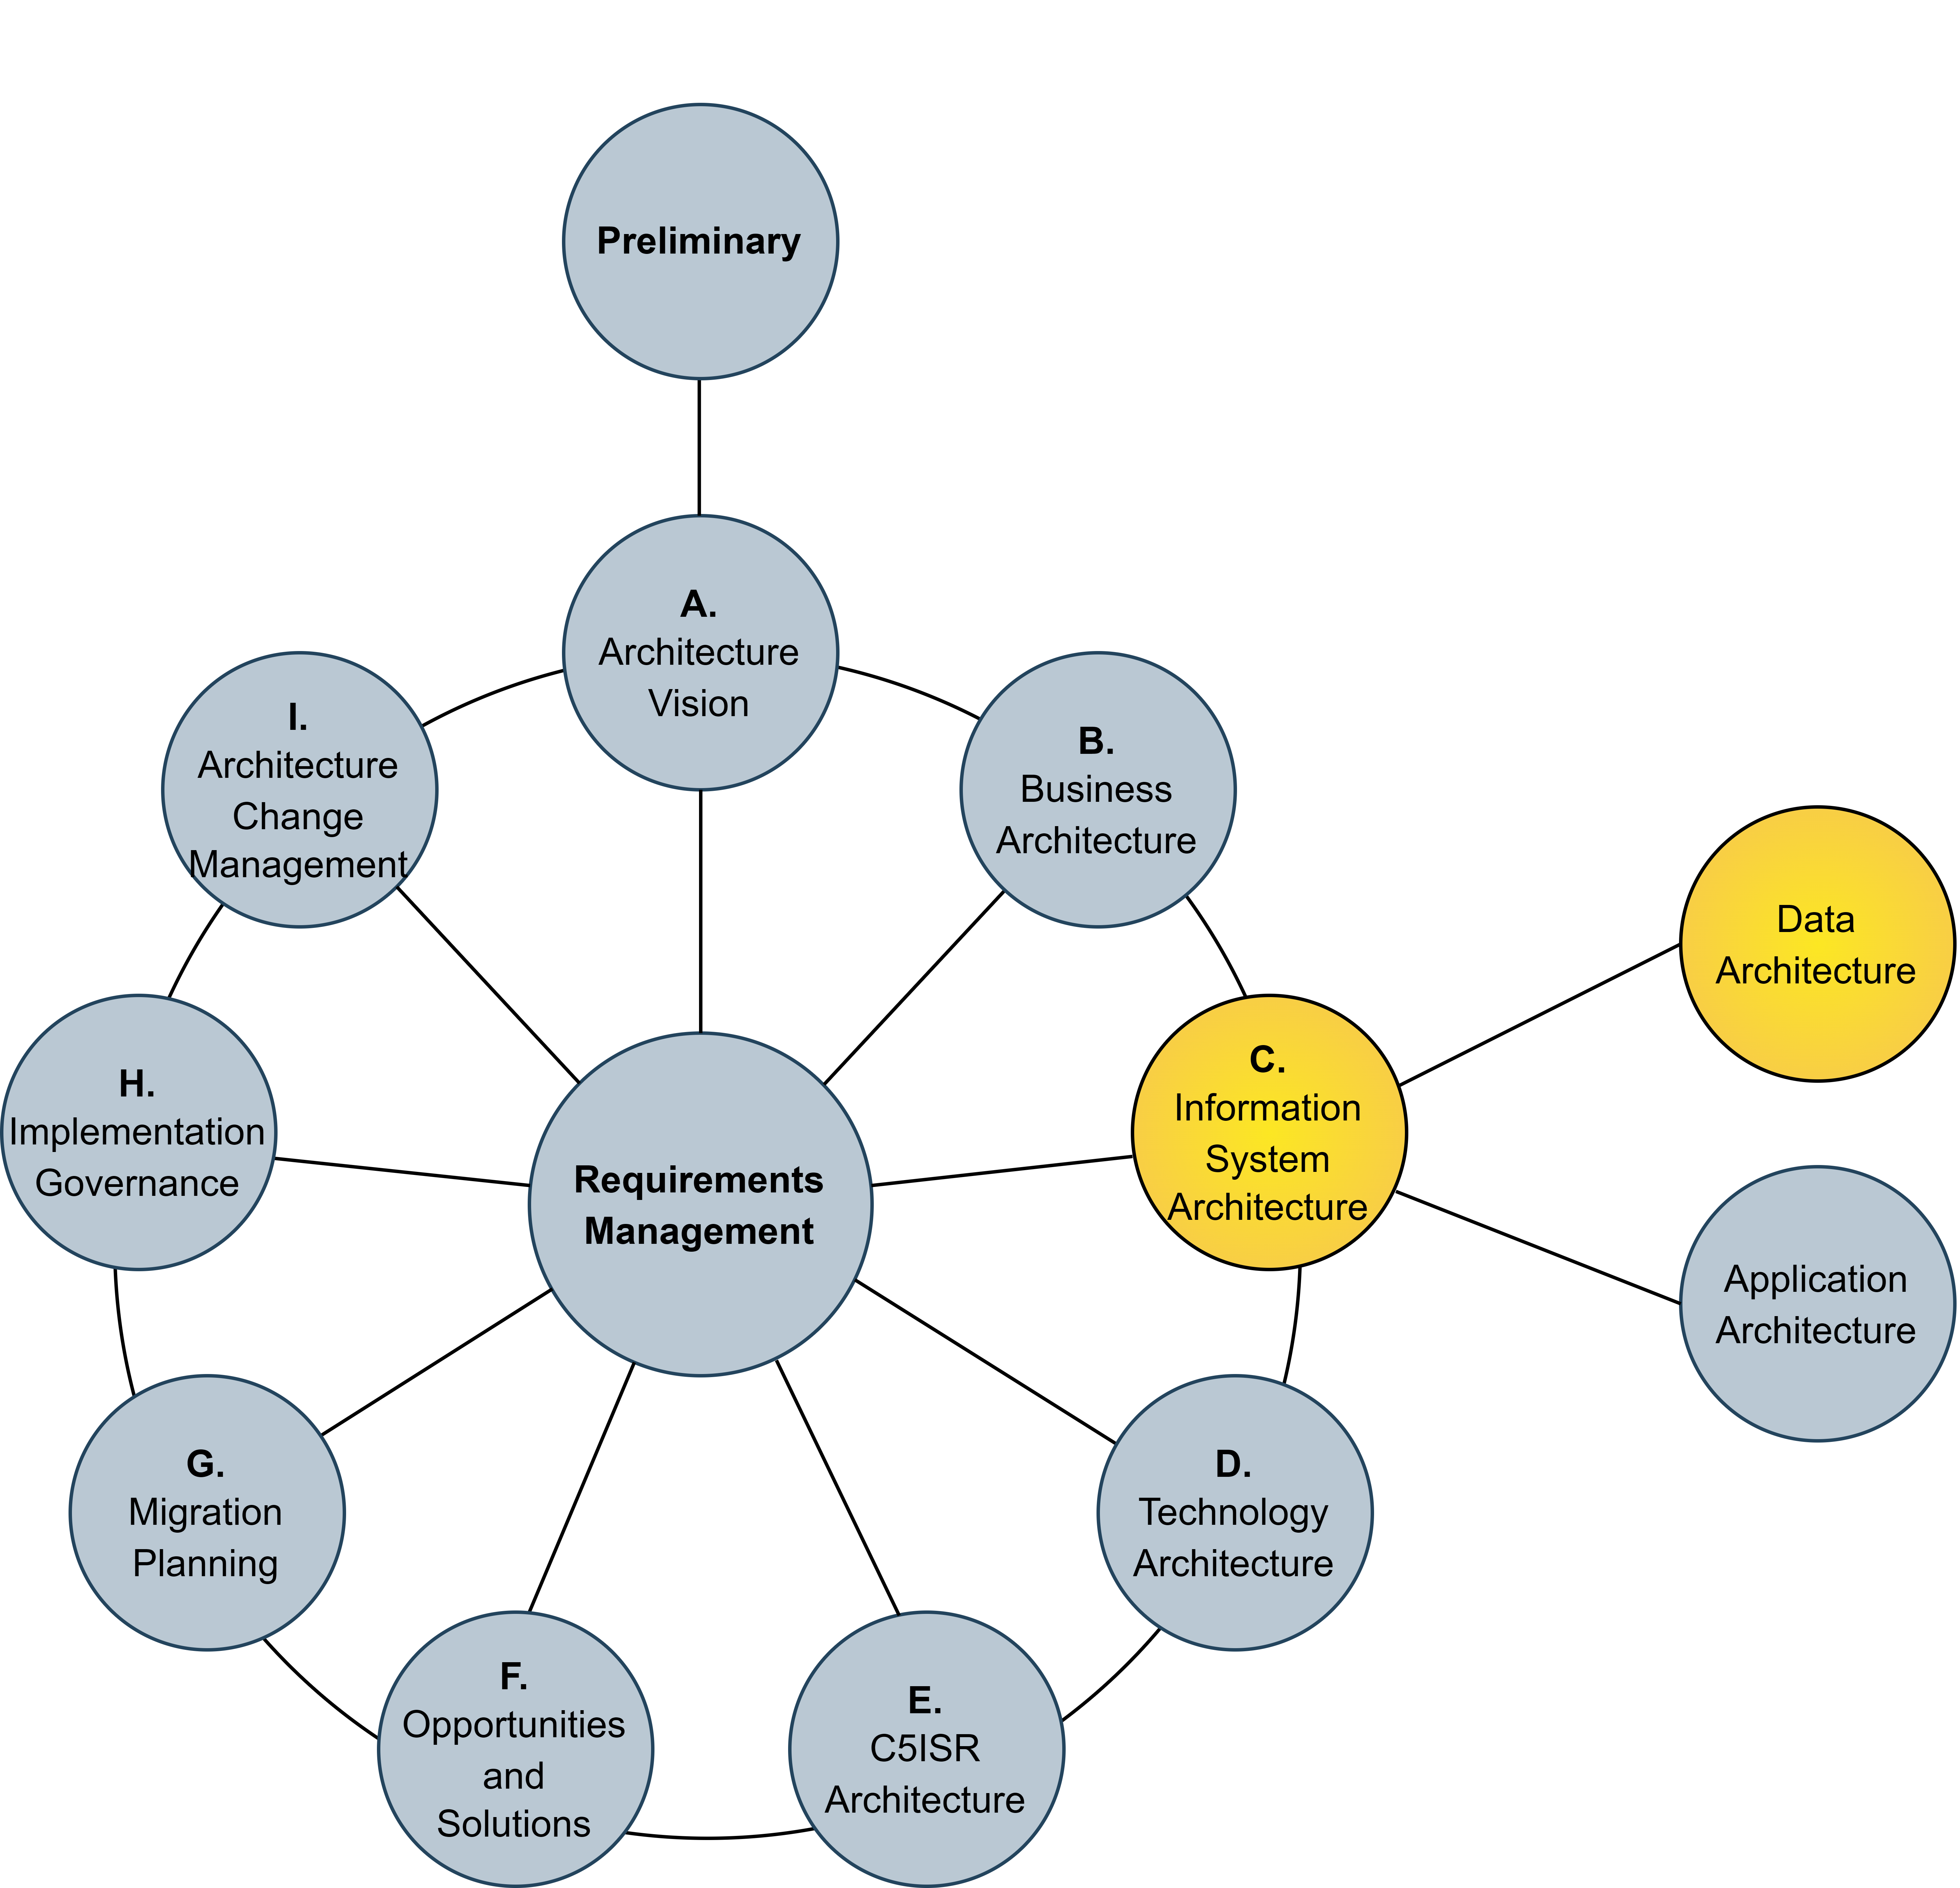
\includegraphics[width=0.42\textwidth]{images/Data Architecture.drawio.png}
\end{figure}

Gambar~\ref{fig:fase-data} menunjukkan bahwa arsitektur data merupakan salah satu dari dua cabang fase \textit{Information Systems Architecture} yang dikerjakan terlebih dahulu. \textit{Input}, \textit{step}, dan \textit{output} yang membentuk arsitektur data disajikan pada Tabel~\ref{tab:data-architecture}.

\begin{longtable}{@{}p{0.31\textwidth}p{0.31\textwidth}p{0.31\textwidth}@{}}
\caption{\textit{Input}, \textit{Step}, dan \textit{Output} Sub-domain \textit{Data Architecture}}
\label{tab:data-architecture}\\
\toprule
\textbf{\textit{INPUT}} & \textbf{\textit{STEP}} & \textbf{\textit{OUTPUT}}\\
\midrule
\endfirsthead
\multicolumn{3}{c}{\tablename\ \thetable\ (lanjutan)}\\
\toprule
\textbf{\textit{INPUT}} & \textbf{\textit{STEP}} & \textbf{\textit{OUTPUT}}\\
\midrule
\endhead
\bottomrule
\endfoot
\raggedright
1. \textit{Architecture reference materials}\newline
2. \textit{Request for Architecture Work}\newline
3. Hasil penilaian kapabilitas\newline
4. Rencana komunikasi\newline
5. Model organisasi untuk arsitektur \textit{enterprise}\newline
6. TOGAF Pertahanan Indonesia\newline
7. Prinsip data (\textit{data principles})\newline
8. \textit{Statement of Architecture Work}\newline
9. Dokumen \textit{Architecture Vision}\newline
10. \textit{Architecture Repository}\newline
11. Draf \textit{Architecture Definition Document} dan draf \textit{Architecture Requirements Specification}\newline
12. Komponen arsitektur bisnis pada \textit{roadmap} arsitektur\newline
13. Regulasi nasional dan sektor pertahanan tentang data, mencakup Satu Data Indonesia\newline
14. Standar keamanan siber dan pelindungan data pertahanan
&
\raggedright
1. Memilih model rujukan, sudut pandang, dan perangkat pemodelan data\newline
2. Menyusun deskripsi arsitektur data \textit{baseline}\newline
3. Memodelkan entitas data utama dan hubungan antarsistem pertahanan\newline
4. Menyusun klasifikasi data pertahanan menurut tingkat kerahasiaan\newline
5. Menetapkan kepemilikan dan tata kelola data antarsatuan\newline
6. Menyusun deskripsi arsitektur data target\newline
7. Melakukan analisis kesenjangan (\textit{as-is vs to-be})\newline
8. Menetapkan komponen \textit{roadmap} arsitektur data\newline
9. Melaksanakan tinjauan formal pemangku kepentingan\newline
10. Menyelesaikan arsitektur data\newline
11. Menyusun atau memperbarui \textit{Architecture Definition Document}
&
\raggedright
1. Versi yang diperhalus dan diperbarui dari keluaran fase \textit{Architecture Vision}\newline
2. Draf \textit{Architecture Definition Document}\newline
3. Draf \textit{Architecture Requirements Specification}\newline
4. Komponen arsitektur data pada \textit{roadmap} arsitektur\newline
5. Model entitas data pertahanan\newline
6. Klasifikasi data pertahanan menurut tingkat kerahasiaan\newline
7. Kamus data dan standar penamaan data pertahanan\newline
8. Matriks kepemilikan dan tata kelola data antarsatuan\newline
9. Rancangan \textit{data security and access control}\arraybackslash\\
\end{longtable}

\textit{Input} pada sub-domain ini menghadirkan ketentuan yang mengikat pengelolaan data pertahanan, yaitu regulasi tentang data termasuk Satu Data Indonesia serta standar keamanan siber dan pelindungan data. Kedua masukan tersebut menjadi pembatas sekaligus pengarah, karena rancangan data yang dihasilkan harus memenuhi kewajiban berbagi pakai data sekaligus menghormati ketentuan kerahasiaan.

Langkah-langkah dari sub-domain ini dipusatkan pada penataan data yang selama ini terkotak antarsatuan. Pemodelan entitas data utama, penyusunan klasifikasi data menurut tingkat kerahasiaan, dan penetapan kepemilikan data antarsatuan merupakan inti pekerjaan yang menjadikan data dapat dibagipakaikan menurut aturan yang jelas. Tanpa klasifikasi yang tegas, setiap satuan cenderung memilih sikap paling aman dengan tidak membagikan data sama sekali.

\textit{Output} sub-domain ini menjadi rujukan tunggal bagi pengelolaan data. Model entitas data, klasifikasi kerahasiaan, kamus data, dan matriks kepemilikan menetapkan siapa yang bertanggung jawab atas setiap kumpulan data, sedangkan rancangan \textit{data security and access control} menjadi masukan langsung bagi arsitektur aplikasi dan bagi perancangan fondasi keamanan siber pada fase \textit{Technology Architecture}.

\paragraph{\textit{Application Architecture}}\mbox{}\\
Arsitektur aplikasi dilakukan untuk merancang portofolio aplikasi yang diperlukan untuk menjalankan proses bisnis pertahanan serta menetapkan mekanisme keterhubungan antaraplikasi. Perancangan arsitektur aplikasi berpedoman pada prinsip \textit{Interoperabilitas} dan prinsip \textit{User-Centric Service}. Kedudukan sub-domain ini dalam siklus TOGAF Pertahanan Indonesia ditunjukkan pada Gambar~\ref{fig:fase-aplikasi}.

\begin{figure}[htbp]
\centering
\caption{Kedudukan Sub-domain \textit{Application Architecture} pada Siklus TOGAF Pertahanan Indonesia}
\label{fig:fase-aplikasi}
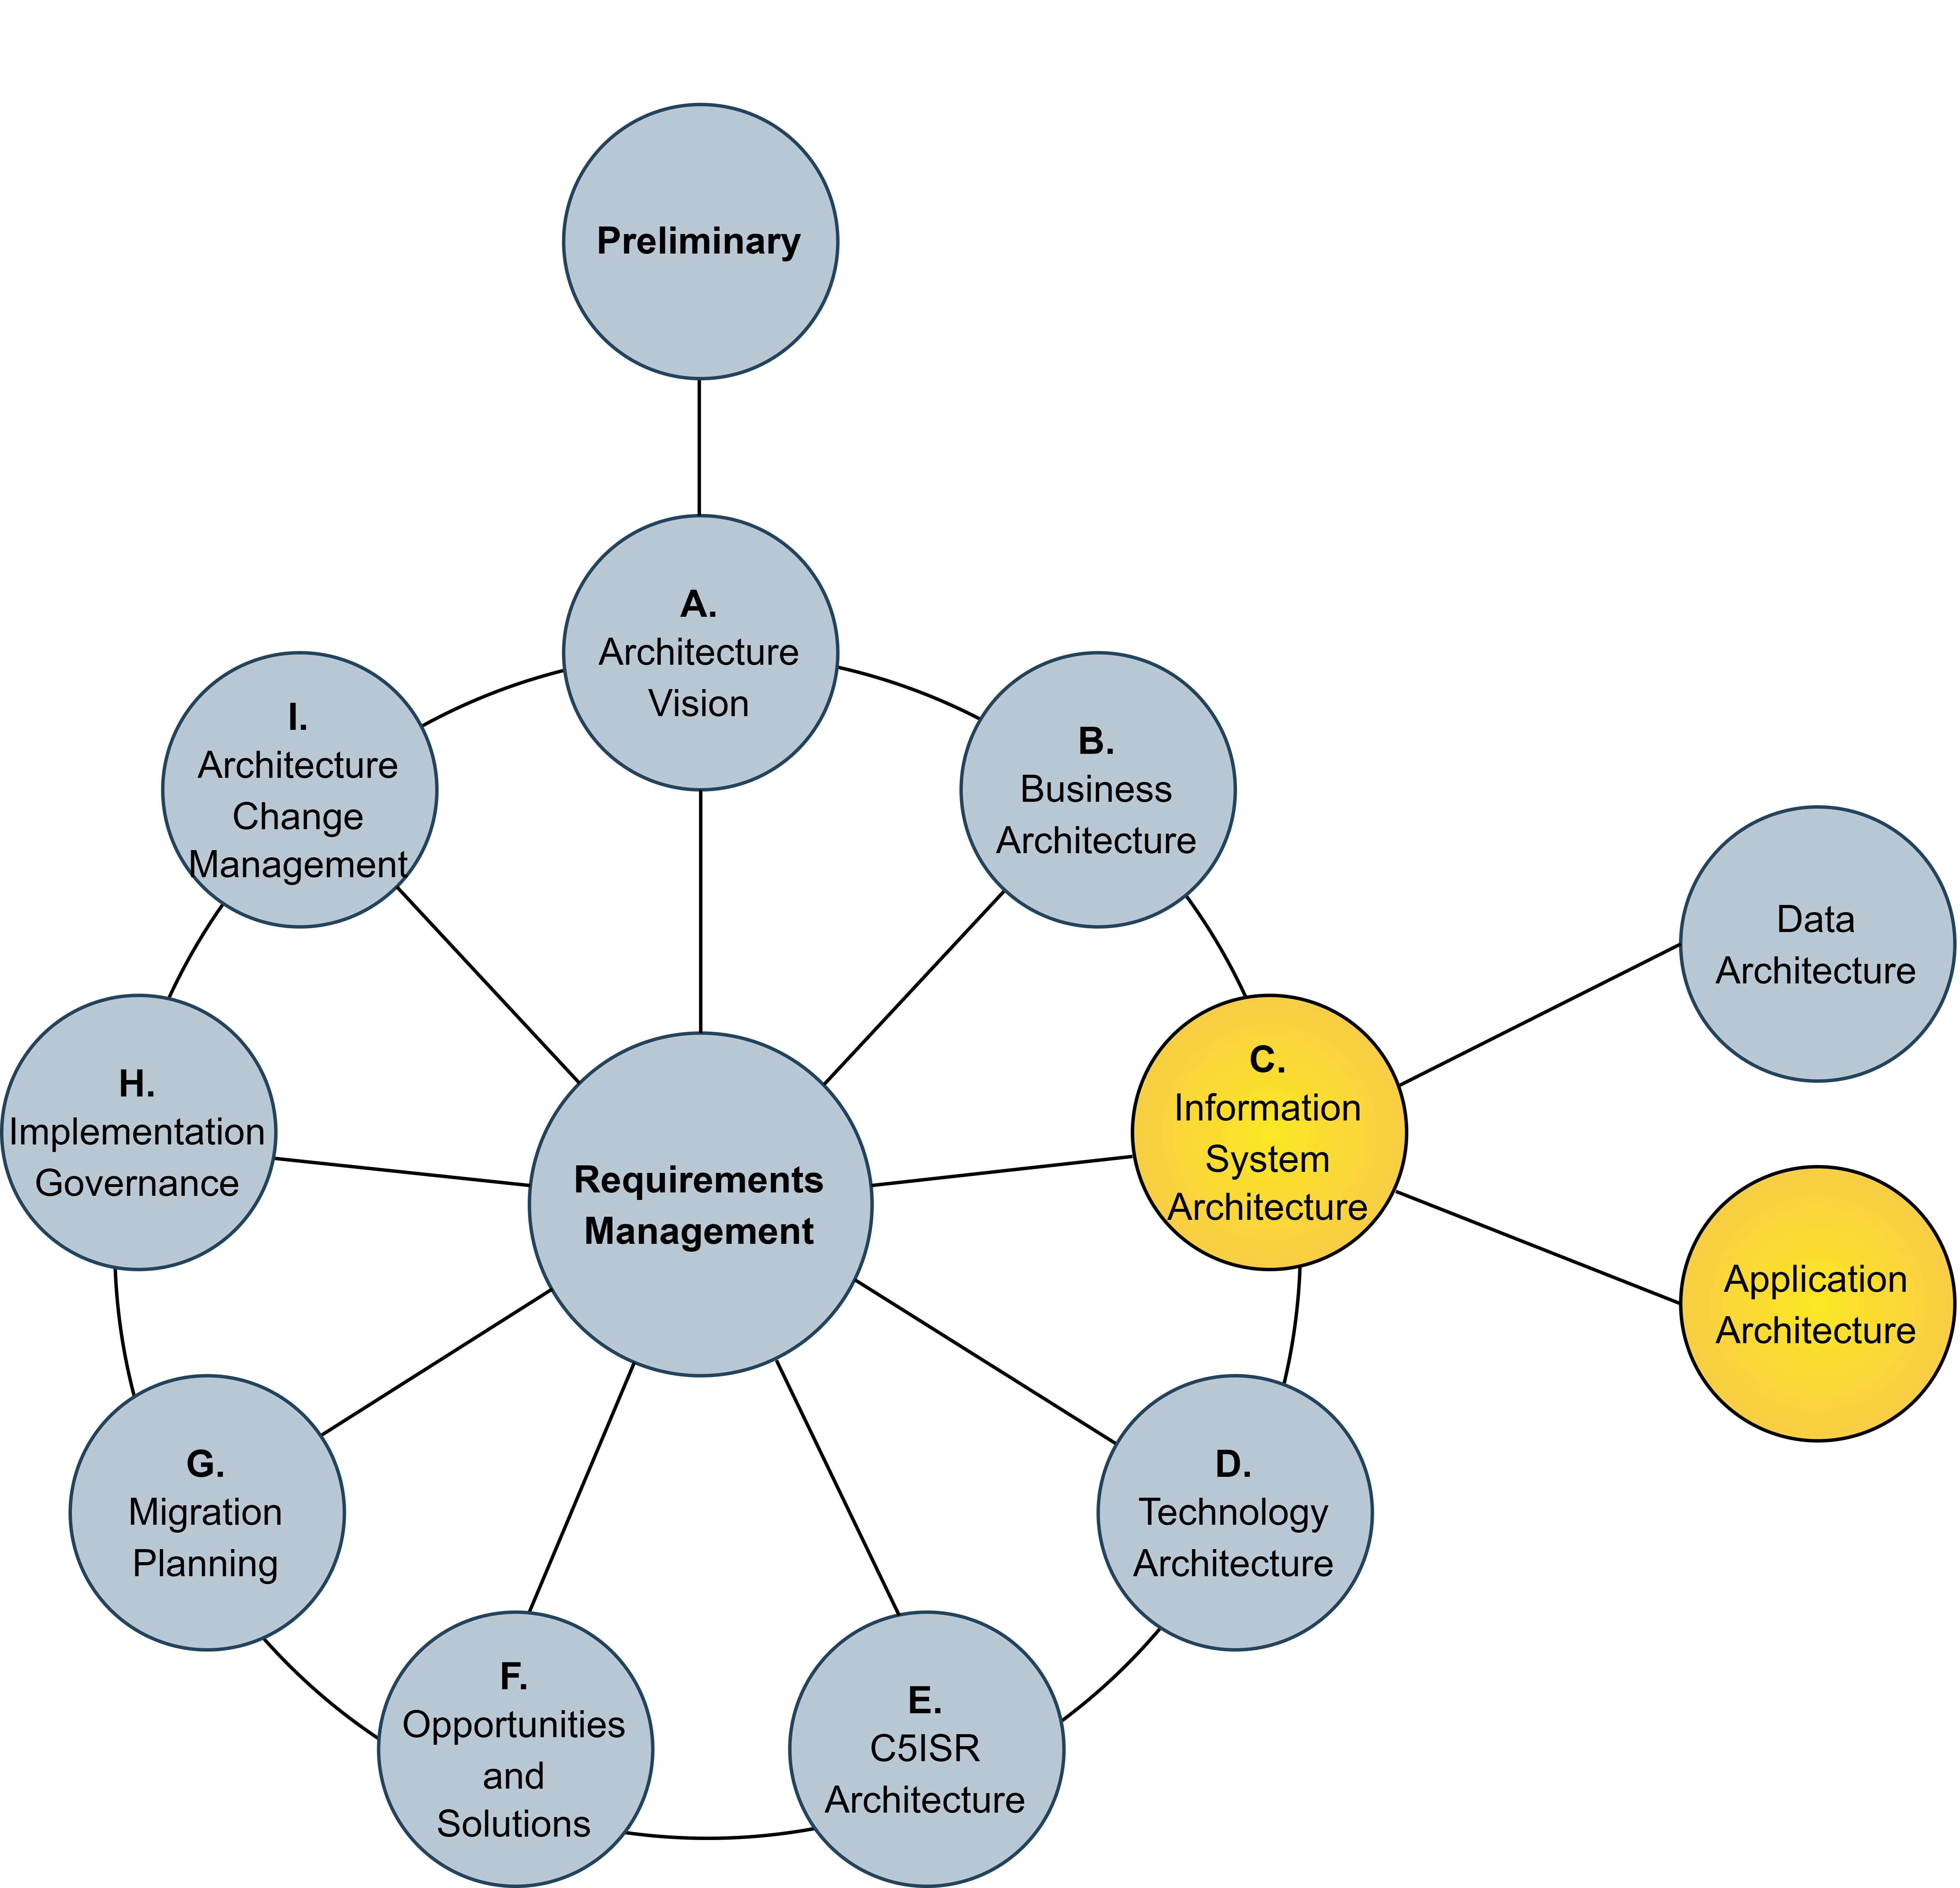
\includegraphics[width=0.42\textwidth]{images/Application Architecture.drawio.png}
\end{figure}

Gambar~\ref{fig:fase-aplikasi} menunjukkan arsitektur aplikasi sebagai cabang kedua fase \textit{Information Systems Architecture}, yang dikerjakan setelah arsitektur data selesai ditetapkan. Fokusnya adalah menentukan aplikasi apa yang dibutuhkan, aplikasi mana yang masih layak dipertahankan, dan bagaimana aplikasi lintas satuan dapat saling bertukar data. Rincian \textit{input}, \textit{step}, dan \textit{output} dapat dilihat pada Tabel~\ref{tab:application-architecture}.

\begin{longtable}{@{}p{0.31\textwidth}p{0.31\textwidth}p{0.31\textwidth}@{}}
\caption{\textit{Input}, \textit{Step}, dan \textit{Output} Sub-domain \textit{Application Architecture}}
\label{tab:application-architecture}\\
\toprule
\textbf{INPUT} & \textbf{STEP} & \textbf{OUTPUT}\\
\midrule
\endfirsthead
\multicolumn{3}{c}{\tablename\ \thetable\ (lanjutan)}\\
\toprule
\textbf{INPUT} & \textbf{STEP} & \textbf{OUTPUT}\\
\midrule
\endhead
\bottomrule
\endfoot
\raggedright
1. \textit{Architecture reference materials}\newline
2. \textit{Request for Architecture Work}\newline
3. Hasil penilaian kapabilitas\newline
4. Rencana komunikasi\newline
5. Model organisasi untuk arsitektur \textit{enterprise}\newline
6. TOGAF Pertahanan Indonesia\newline
7. Prinsip aplikasi (\textit{application principles})\newline
8. \textit{Statement of Architecture Work}\newline
9. Dokumen \textit{Architecture Vision}\newline
10. \textit{Architecture Repository}\newline
11. Draf \textit{Architecture Definition Document} dan draf \textit{Architecture Requirements Specification}\newline
12. Komponen arsitektur bisnis pada \textit{roadmap} arsitektur\newline
13. Komponen arsitektur data pada \textit{roadmap} arsitektur\newline
14. Standar interoperabilitas dan integrasi lintas matra
&
\raggedright
1. Memilih model rujukan, sudut pandang, dan perangkat pemodelan aplikasi\newline
2. Menyusun deskripsi arsitektur aplikasi \textit{baseline} melalui inventarisasi aplikasi Kemhan dan TNI\newline
3. Menyusun deskripsi arsitektur aplikasi target\newline
4. Merancang portofolio aplikasi pendukung operasi dan administrasi pertahanan\newline
5. Merancang mekanisme integrasi dan pertukaran data lintas matra (\textit{data exchange})\newline
6. Melakukan analisis kesenjangan (\textit{as-is vs to-be})\newline
7. Menetapkan komponen \textit{roadmap} arsitektur aplikasi\newline
8. Melaksanakan tinjauan formal pemangku kepentingan\newline
9. Menyelesaikan arsitektur aplikasi\newline
10. Menyusun atau memutakhirkan \textit{Architecture Definition Document}
&
\raggedright
1. Versi yang diperhalus dan diperbarui dari keluaran fase \textit{Architecture Vision}\newline
2. Draf \textit{Architecture Definition Document}\newline
3. Draf \textit{Architecture Requirements Specification}\newline
4. Komponen arsitektur aplikasi pada \textit{roadmap} arsitektur\newline
5. Portofolio aplikasi pertahanan\newline
6. Peta keterkaitan aplikasi dengan kapabilitas dan proses bisnis pertahanan\newline
7. Rancangan mekanisme integrasi dan pertukaran data lintas matra\newline
8. Daftar aplikasi yang dipertahankan, digabungkan, atau dihentikan\arraybackslash\\
\end{longtable}

\textit{Input} pada sub-domain ini mencakup keluaran arsitektur data, khususnya kamus data dan aturan akses, serta standar interoperabilitas dan integrasi lintas matra. Ketergantungan pada keluaran arsitektur data inilah yang menjadi alasan arsitektur aplikasi dikerjakan setelahnya, sebab keterhubungan antaraplikasi hanya dapat dirancang di atas definisi data yang telah disepakati.

Langkah-langkah pada sub-domain ini dimulai dari inventarisasi aplikasi yang berjalan di lingkungan Kemhan dan TNI, dilanjutkan dengan perancangan portofolio aplikasi target dan mekanisme pertukaran data lintas matra. Rangkaian ini diarahkan tidak hanya untuk menambah aplikasi baru, tetapi juga untuk menata aplikasi yang sudah ada agar tidak saling tumpang tindih.

\textit{Output} dari sub-domain ini menegaskan orientasi rasionalisasi. Portofolio aplikasi, peta keterkaitan aplikasi dengan kapabilitas dan proses bisnis, serta daftar aplikasi yang dipertahankan, digabungkan, atau dihentikan memberikan dasar bagi penataan aplikasi pertahanan secara menyeluruh. Rancangan mekanisme integrasi lintas matra yang dihasilkan bekerja di atas klasifikasi dan aturan akses dari arsitektur data, sehingga pertukaran data berlangsung menurut aturan yang telah disepakati.

\subsubsection{Fase \textit{Technology Architecture}}

Pada fase \textit{Technology Architecture} disusun arsitektur teknologi yang mencakup infrastruktur jaringan, pusat data, komputasi awan dan tepi, serta fondasi keamanan siber. Arsitektur teknologi ini menjadi landasan fisik dan logis bagi seluruh ekosistem digital pertahanan, sehingga menentukan kelayakan penerapan rancangan arsitektur bisnis, data, dan aplikasi yang telah disusun sebelumnya.

\begin{figure}[htbp]
\centering
\caption{Kedudukan Fase \textit{Technology Architecture} pada Siklus TOGAF Pertahanan Indonesia}
\label{fig:fase-teknologi}
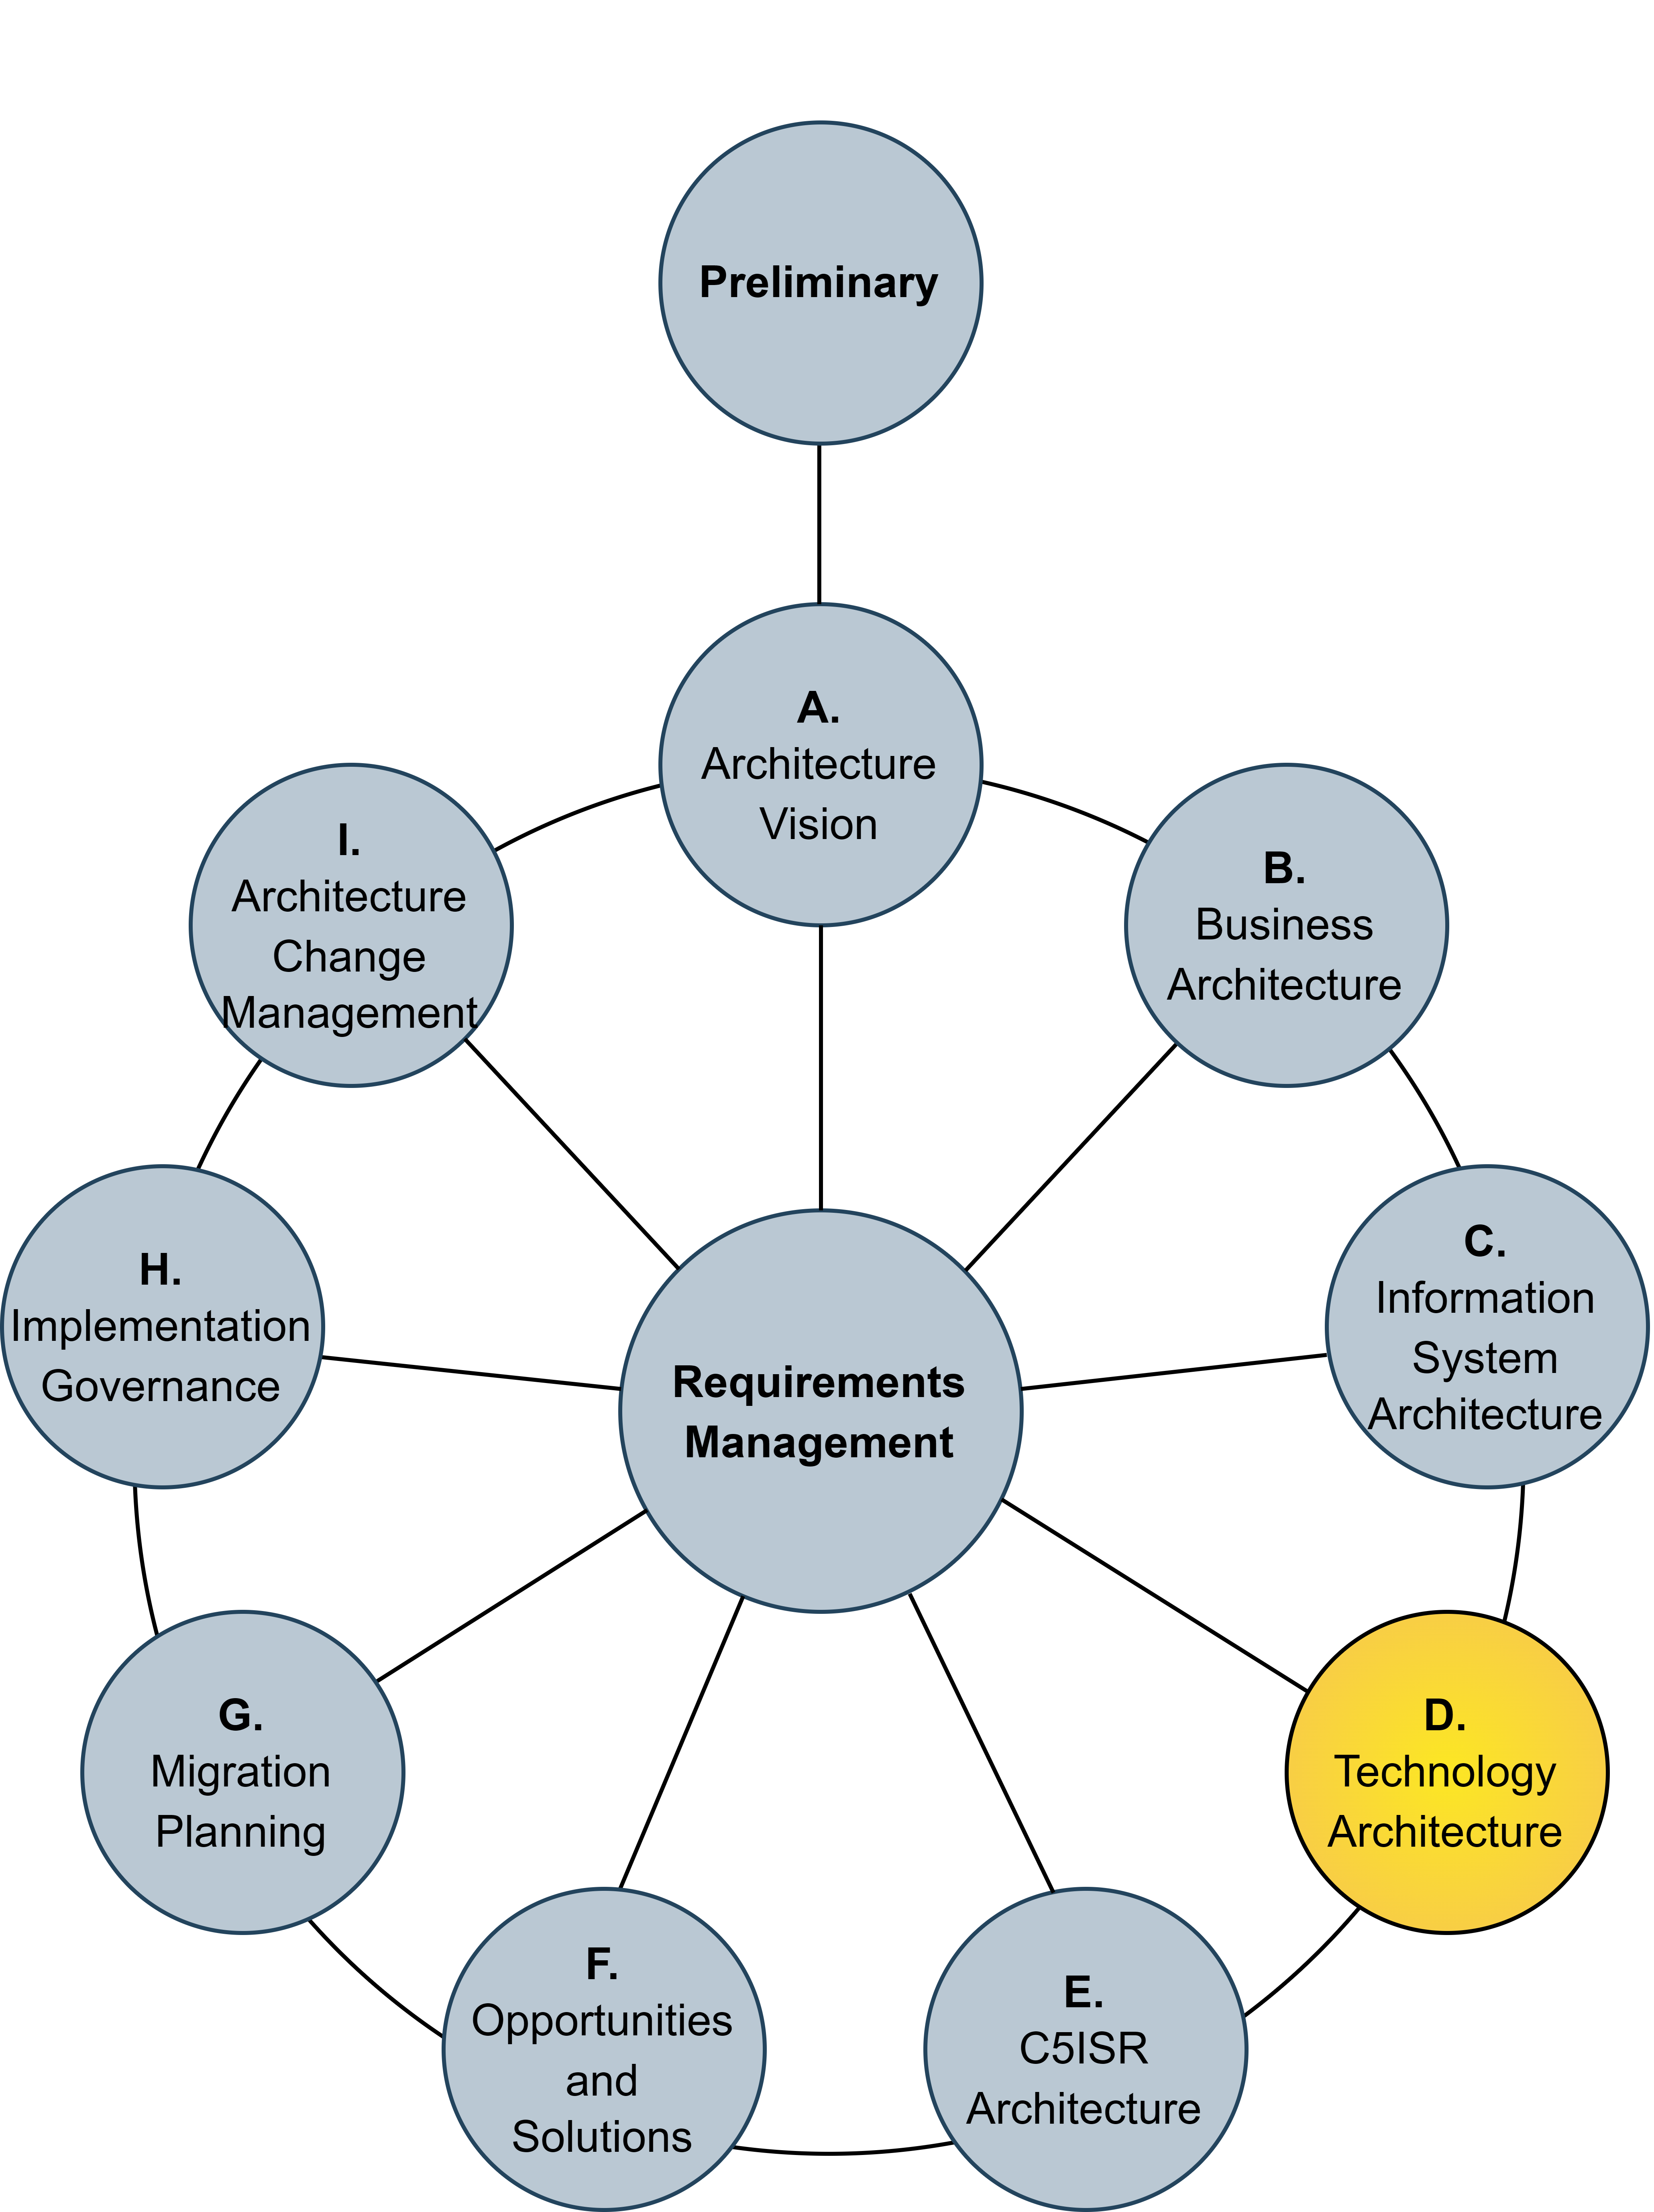
\includegraphics[width=0.42\textwidth]{images/Technology Architecture.drawio.png}
\end{figure}

Gambar~\ref{fig:fase-teknologi} menempatkan fase \textit{Technology Architecture} sebelum fase \textit{C5ISR Architecture}. Posisi ini menegaskan perannya sebagai penyedia fondasi teknologi yang menentukan kelayakan penerapan seluruh rancangan sebelumnya. \textit{Input}, \textit{step}, dan \textit{output} disajikan pada Tabel~\ref{tab:technology-architecture}.

\begin{longtable}{@{}p{0.31\textwidth}p{0.31\textwidth}p{0.31\textwidth}@{}}
\caption{\textit{Input}, \textit{Step}, dan \textit{Output} Fase \textit{Technology Architecture}}
\label{tab:technology-architecture}\\
\toprule
\textbf{INPUT} & \textbf{STEP} & \textbf{OUTPUT}\\
\midrule
\endfirsthead
\multicolumn{3}{c}{\tablename\ \thetable\ (lanjutan)}\\
\toprule
\textbf{INPUT} & \textbf{STEP} & \textbf{OUTPUT}\\
\midrule
\endhead
\bottomrule
\endfoot
\raggedright
1. \textit{Architecture reference materials}\newline
2. Informasi produk atas kandidat teknologi\newline
3. \textit{Request for Architecture Work}\newline
4. Hasil penilaian kapabilitas dan rencana komunikasi\newline
5. Model organisasi untuk arsitektur \textit{enterprise}\newline
6. TOGAF Pertahanan Indonesia\newline
7. Prinsip teknologi dan spesifikasi kebutuhan standar\newline
8. \textit{Statement of Architecture Work} dan dokumen \textit{Architecture Vision}\newline
9. \textit{Architecture Repository}\newline
10. Draf \textit{Architecture Definition Document} dan draf \textit{Architecture Requirements Specification}\newline
11. Komponen arsitektur data dan aplikasi pada \textit{roadmap} arsitektur\newline
12. Kebutuhan keamanan siber pertahanan
&
\raggedright
1. Memilih model rujukan, sudut pandang, dan perangkat pemodelan\newline
2. Mendeskripsikan arsitektur teknologi \textit{baseline}\newline
3. Menyusun deskripsi arsitektur teknologi target yang mencakup jaringan, \textit{server}, \textit{cloud}, dan \textit{edge}\newline
4. Merancang fondasi keamanan siber terpadu lintas lapisan\newline
5. Menetapkan standar teknologi dan protokol keamanan pertahanan\newline
6. Melakukan analisis kesenjangan\newline
7. Menetapkan komponen \textit{roadmap}\newline
8. Menyelesaikan dampak lintas lanskap arsitektur\newline
9. Melaksanakan tinjauan formal pemangku kepentingan\newline
10. Memfinalkan arsitektur teknologi\newline
11. Menyusun \textit{Architecture Definition Document}
&
\raggedright
1. Versi yang diperhalus dan dimutakhirkan dari keluaran fase \textit{Architecture Vision}\newline
2. Draf \textit{Architecture Definition Document}\newline
3. Draf \textit{Architecture Requirements Specification}\newline
4. Komponen teknologi pada \textit{roadmap} arsitektur\newline
5. Model arsitektur teknologi pertahanan\newline
6. Standar teknologi dan protokol keamanan\newline
7. Rancangan fondasi keamanan siber terpadu\arraybackslash\\
\end{longtable}

\textit{Input} fase ini bertumpu pada keluaran arsitektur data dan aplikasi, ditambah kebutuhan keamanan siber pertahanan sebagai masukan khas. Kehadiran kebutuhan keamanan siber sejak awal fase menandakan bahwa keamanan diperlakukan sebagai pertimbangan perancangan, bukan sebagai penyesuaian yang ditambahkan setelah teknologi dipilih.

Langkah-langkah pada fase ini memuat perancangan arsitektur teknologi target yang mencakup jaringan, \textit{server}, komputasi awan, dan komputasi tepi, disertai dua langkah bernilai strategis, yaitu perancangan fondasi keamanan siber terpadu lintas lapisan dan penetapan standar teknologi serta protokol keamanan. Kedua langkah ini merupakan penerapan langsung prinsip \textit{Security by Design}.

\textit{Output} fase ini berupa model arsitektur teknologi pertahanan, standar teknologi dan protokol keamanan, serta rancangan fondasi keamanan siber terpadu. Rancangan fondasi keamanan tersebut menjadi masukan penting bagi fase \textit{C5ISR Architecture}, sehingga kapabilitas komando dan kendali dibangun di atas landasan keamanan yang telah ditetapkan, bukan di atas landasan yang masih harus disiapkan kemudian.

\subsubsection{Fase \textit{C5ISR Architecture}}

Fase \textit{C5ISR Architecture} merupakan fase khusus yang terdapat pada TOGAF Pertahanan Indonesia. Fase ini merancang arsitektur kapabilitas C5ISR, yaitu \textit{Command, Control, Communication, Computer, Cyber, Intelligence, Surveillance, and Reconnaissance}, sebagai inti operasional pertahanan.

\begin{figure}[htbp]
\centering
\caption{Kedudukan Fase \textit{C5ISR Architecture} pada Siklus TOGAF Pertahanan Indonesia}
\label{fig:fase-c5isr}
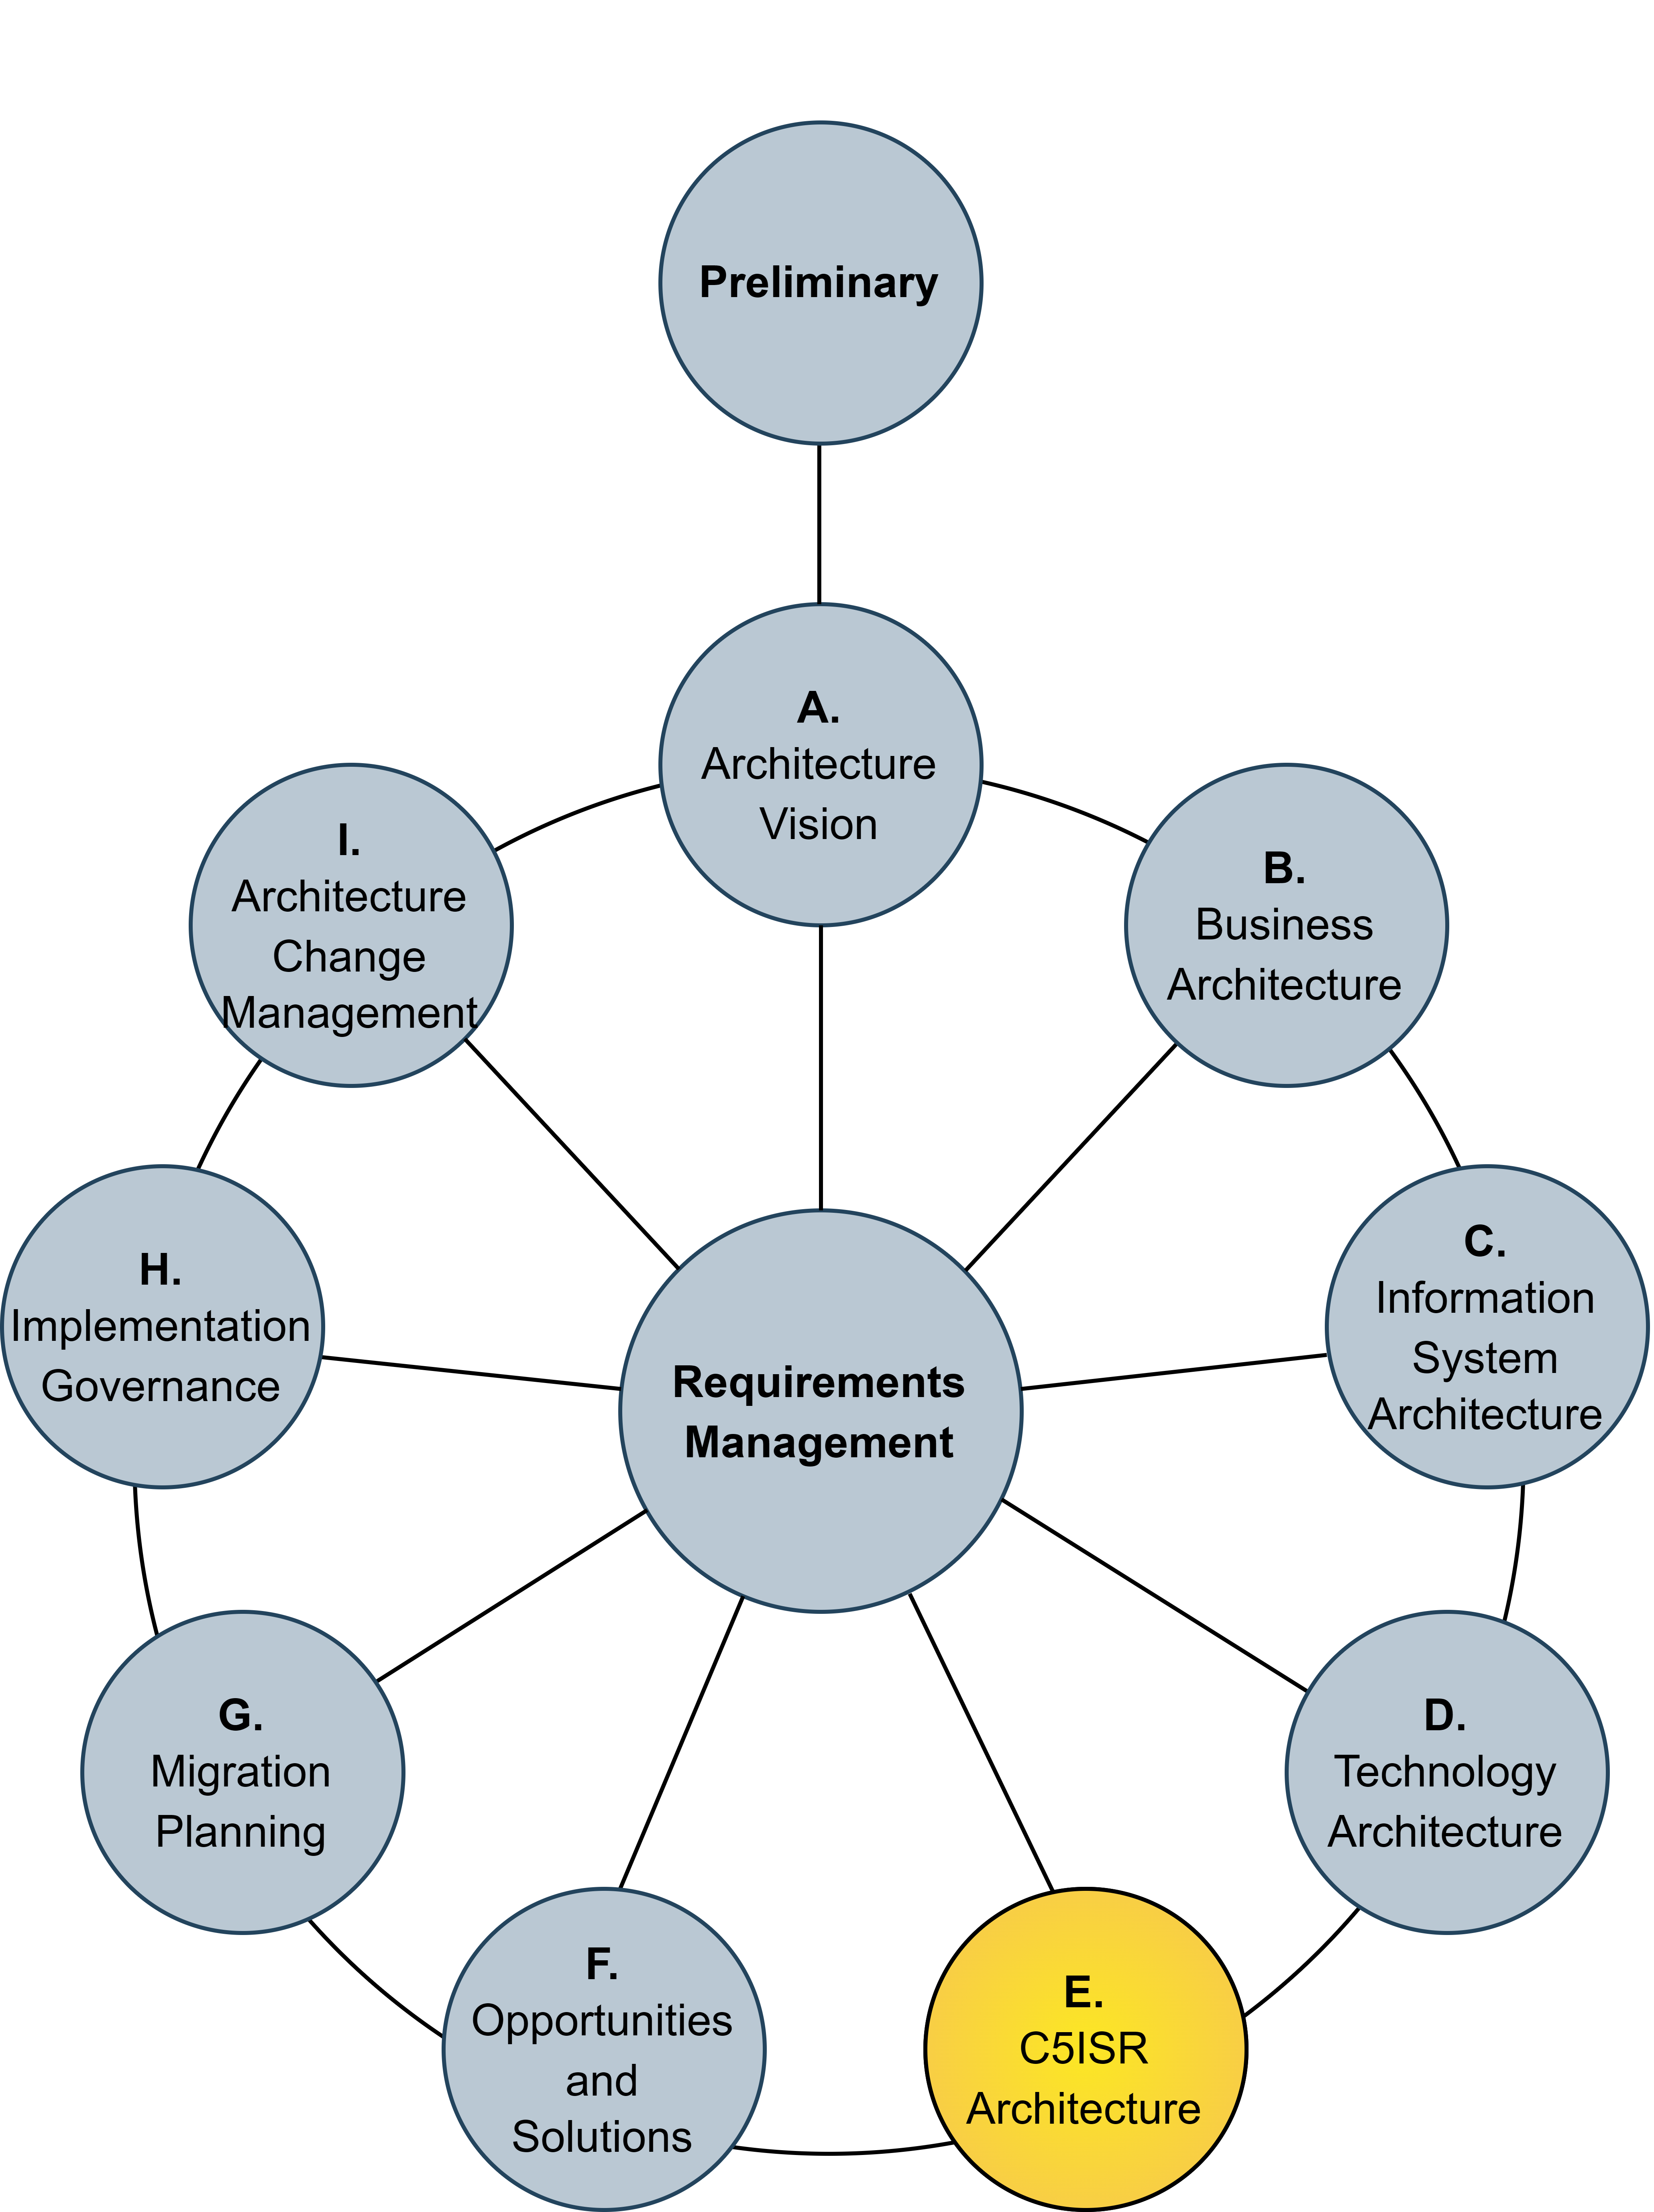
\includegraphics[width=0.42\textwidth]{images/C5ISR Architecture.drawio.png}
\end{figure}

Arsitektur C5ISR dirancang dengan pendekatan \textit{network centric warfare} yang menghubungkan unsur sensor (\textit{surveillance} dan \textit{reconnaissance}), unsur pemroses dan intelijen, unsur pengambil keputusan (\textit{command and control}), serta unsur penindak (\textit{effector}) dalam satu jaringan informasi terpadu.

Gambar~\ref{fig:fase-c5isr} memperlihatkan penempatan fase \textit{C5ISR Architecture} setelah \textit{Technology Architecture} dan sebelum \textit{Opportunities \& Solutions} menegaskan bahwa kapabilitas C5ISR dirancang di atas fondasi data, aplikasi, teknologi, dan keamanan yang telah ditetapkan sebelumnya. \textit{Input}, \textit{step}, dan \textit{output} disajikan pada Tabel~\ref{tab:c5isr-architecture}.

\begin{longtable}{@{}p{0.31\textwidth}p{0.31\textwidth}p{0.31\textwidth}@{}}
\caption{\textit{Input}, \textit{Step}, dan \textit{Output} Fase \textit{C5ISR Architecture}}
\label{tab:c5isr-architecture}\\
\toprule
\textbf{INPUT} & \textbf{STEP} & \textbf{OUTPUT}\\
\midrule
\endfirsthead
\multicolumn{3}{c}{\tablename\ \thetable\ (lanjutan)}\\
\toprule
\textbf{INPUT} & \textbf{STEP} & \textbf{OUTPUT}\\
\midrule
\endhead
\bottomrule
\endfoot
\raggedright
1. Model arsitektur data, aplikasi, dan teknologi dari fase sebelumnya\newline
2. Prinsip arsitektur pertahanan, khususnya \textit{Integrated Command \& Control} dan \textit{Interoperabilitas}\newline
3. Doktrin pertahanan dan kebutuhan \textit{smart defence}\newline
4. Konsep \textit{Network Centric Warfare} dan operasi multi-domain\newline
5. Standar interoperabilitas lintas matra dan lintas entitas\newline
6. Rancangan fondasi keamanan siber terpadu dari fase \textit{Technology Architecture}\newline
7. Draf \textit{Architecture Definition Document} dan draf \textit{Architecture Requirements Specification}
&
\raggedright
1. Memilih model rujukan dan sudut pandang C5ISR, antara lain \textit{operational} dan \textit{systems viewpoint}\newline
2. Memetakan kapabilitas C5ISR dan keterkaitannya dengan proses pertahanan\newline
3. Menyusun deskripsi arsitektur C5ISR \textit{baseline}\newline
4. Merancang arsitektur komando dan kendali terpadu\newline
5. Merancang integrasi unsur sensor, pengambil keputusan, dan penindak dalam satu jaringan (\textit{sensor to effector})\newline
6. Mengintegrasikan pertahanan siber dan operasi lintas domain\newline
7. Menyusun deskripsi arsitektur C5ISR target\newline
8. Melakukan analisis kesenjangan\newline
9. Menetapkan komponen \textit{roadmap} C5ISR\newline
10. Melaksanakan tinjauan formal pemangku kepentingan\newline
11. Memfinalkan arsitektur C5ISR dan memutakhirkan \textit{Architecture Definition Document}
&
\raggedright
1. Model arsitektur C5ISR pertahanan\newline
2. Rancangan jaringan \textit{sensor to effector}\newline
3. Kerangka integrasi multi-domain dan pertahanan siber\newline
4. Draf \textit{Architecture Definition Document} dan \textit{Architecture Requirements Specification} yang dimutakhirkan\newline
5. Komponen arsitektur C5ISR pada \textit{roadmap} arsitektur\arraybackslash\\
\end{longtable}

\textit{Input} fase ini menghimpun keluaran ketiga fase arsitektur sebelumnya beserta rujukan operasional pertahanan, yaitu doktrin, kebutuhan \textit{smart defence}, konsep \textit{network centric warfare}, dan operasi multi-domain. Himpunan dari masukan ini menempatkan arsitektur C5ISR sebagai bagian akhir dari seluruh rancangan teknis sekaligus penerjemah doktrin pertahanan ke dalam rancangan sistem.

Langkah-langkah pada fase ini mulai dari pemilihan sudut pandang, pemetaan kapabilitas C5ISR, penyusunan arsitektur \textit{baseline} dan target, hingga finalisasi. Inti perancangannya terletak pada integrasi unsur sensor, unsur pengambil keputusan, dan unsur penindak dalam satu jaringan, atau rangkaian \textit{sensor to effector}, yang dipadukan dengan pertahanan siber dan operasi lintas domain.

\textit{Output} fase ini berupa model arsitektur C5ISR pertahanan, rancangan jaringan \textit{sensor to effector}, dan kerangka integrasi multi-domain dan pertahanan siber. Ketiga keluaran tersebut merupakan wujud kapabilitas pertahanan cerdas yang menjadi tujuan penelitian.

\subsubsection{Fase \textit{Opportunities \& Solutions}}

Pada fase \textit{Opportunities \& Solutions} dilakukan penggabungan seluruh kesenjangan yang teridentifikasi dari fase arsitektur bisnis, data, aplikasi, teknologi, dan C5ISR, kemudian menerjemahkannya menjadi kelompok inisiatif dan arsitektur transisi.

\begin{figure}[htbp]
\centering
\caption{Kedudukan Fase \textit{Opportunities \& Solutions} pada Siklus TOGAF Pertahanan Indonesia}
\label{fig:fase-opportunities}
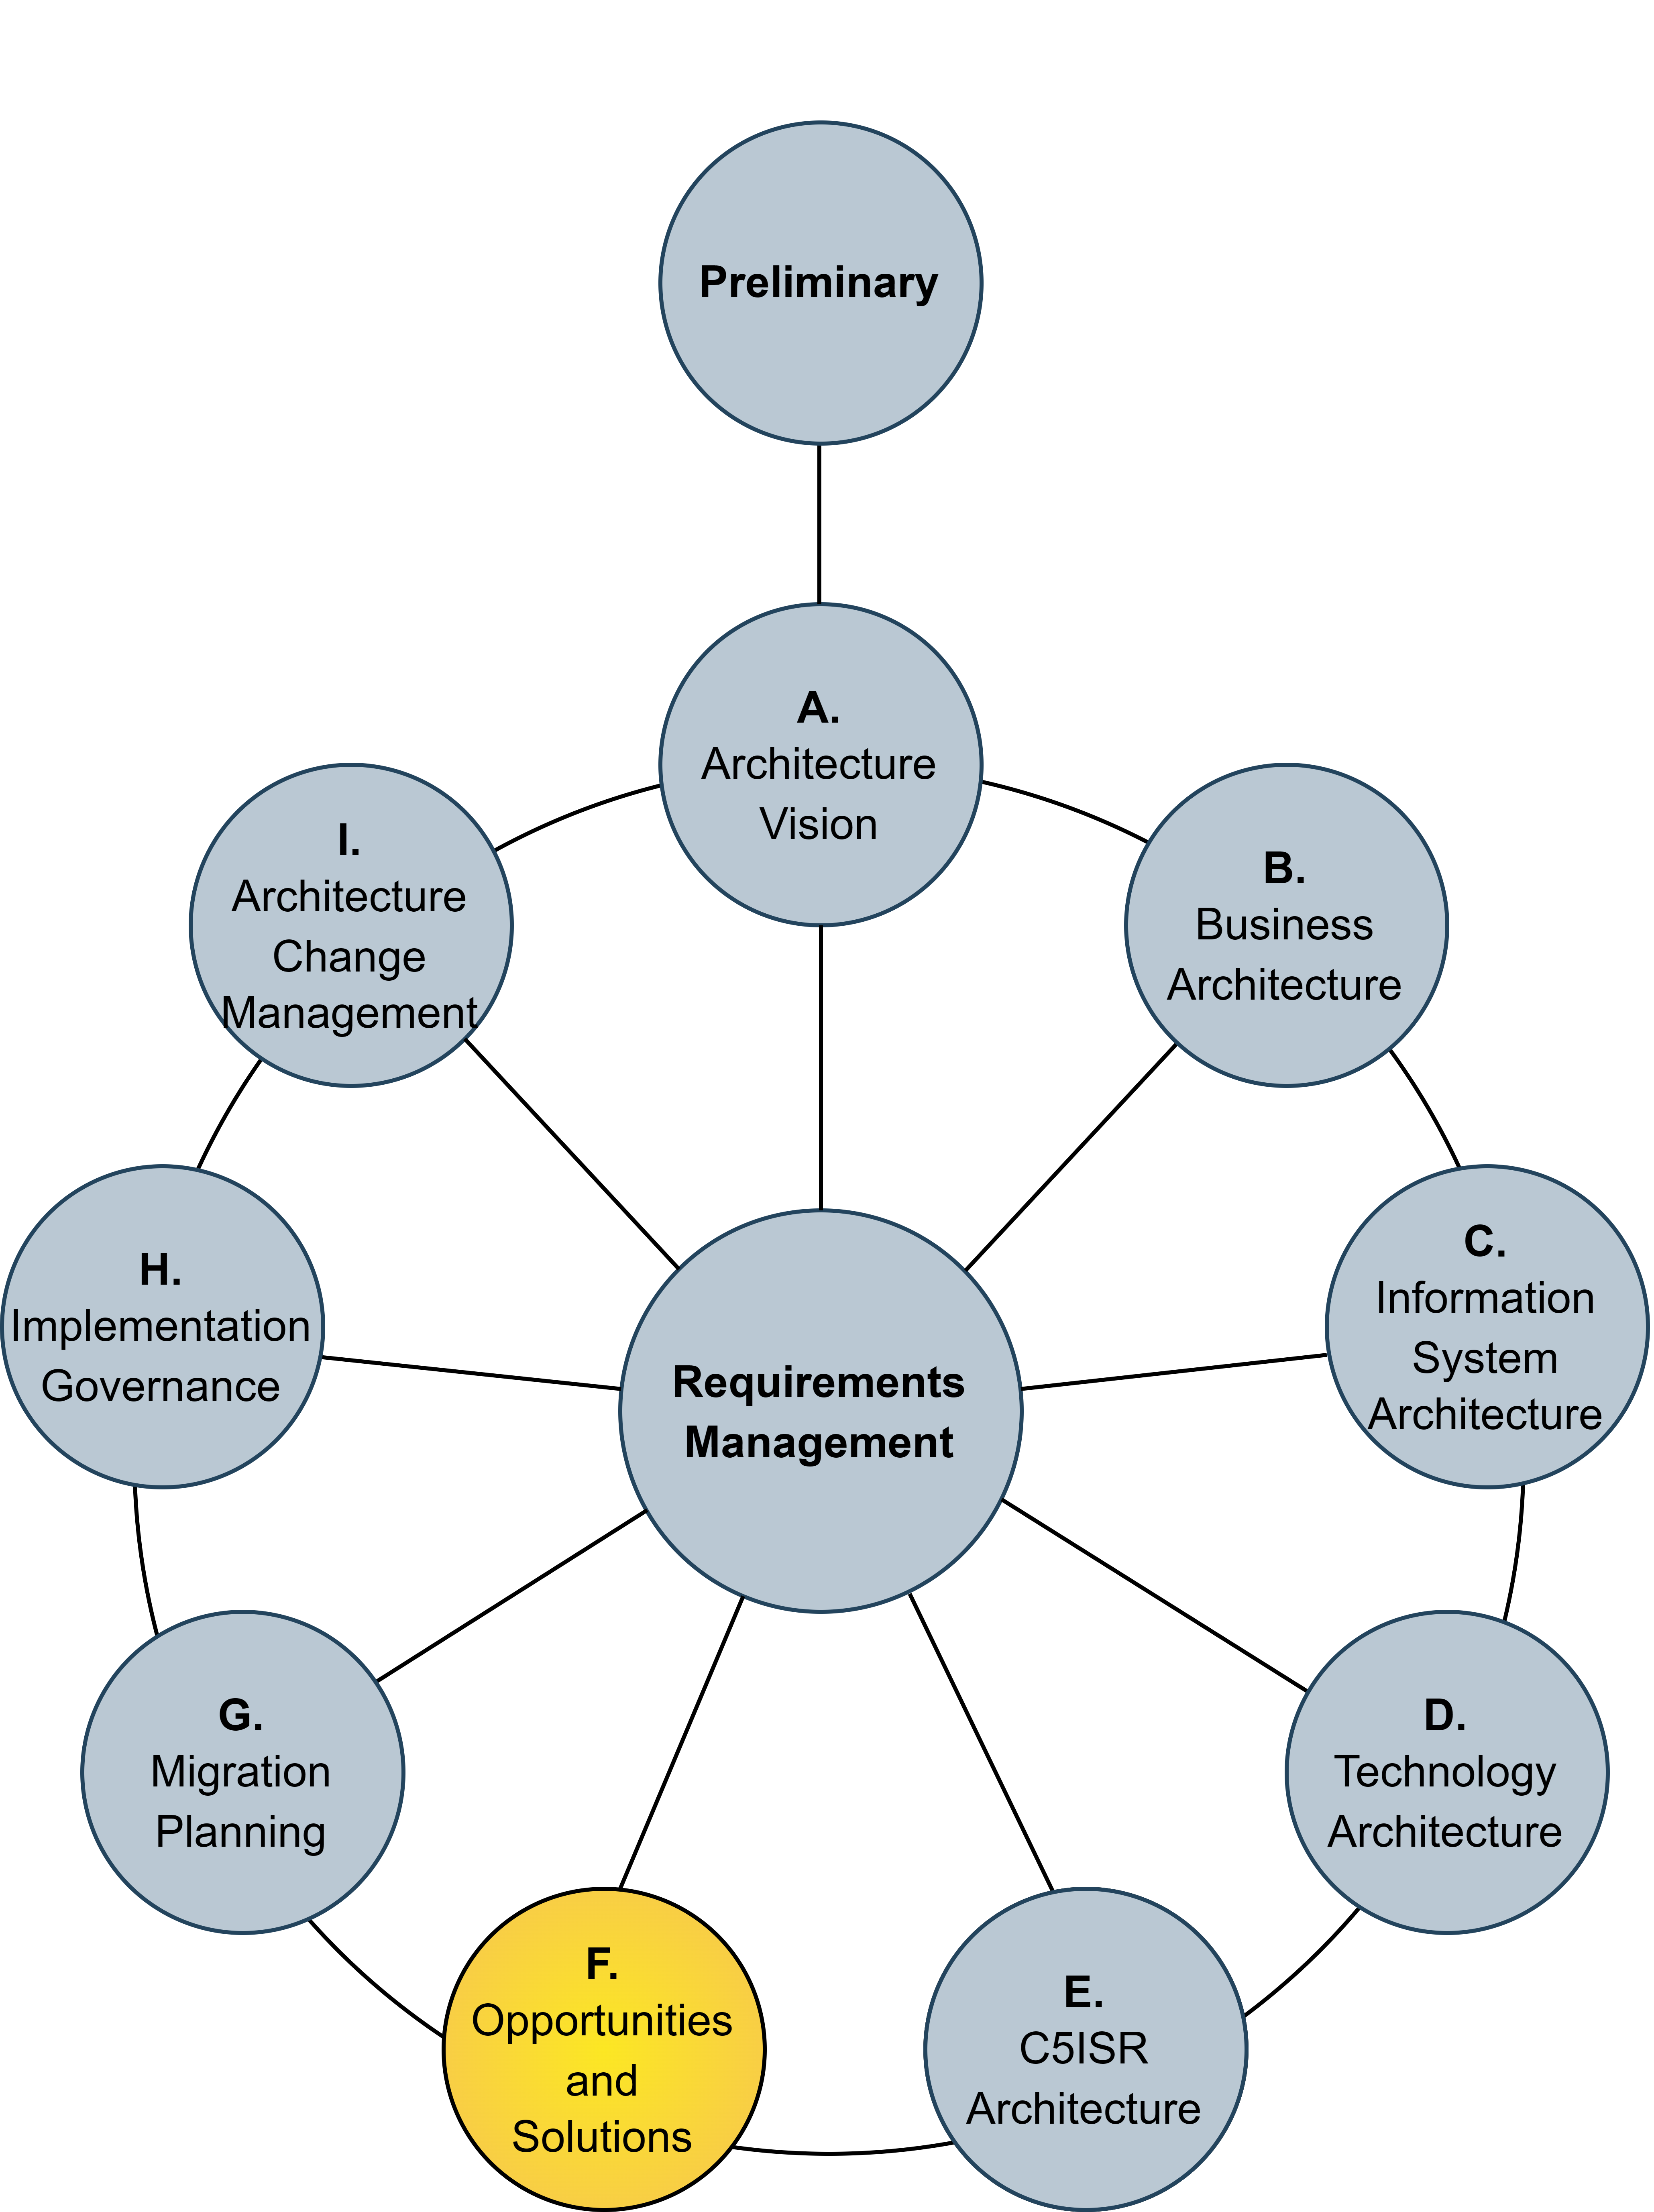
\includegraphics[width=0.42\textwidth]{images/Opportunities & Solutions.drawio.png}
\end{figure}

Gambar~\ref{fig:fase-opportunities} menempatkan fase \textit{Opportunities \& Solutions} sebagai fase pertama dari kelompok realisasi, yaitu titik ketika rancangan arsitektur mulai diterjemahkan menjadi rencana pelaksanaan. Posisi ini menjadikannya penghubung antara kelima fase perancangan sebelumnya dan fase-fase implementasi sesudahnya. \textit{Input}, \textit{step}, dan \textit{output} dapat dilihat pada Tabel~\ref{tab:opportunities-solutions}.

\begin{longtable}{@{}p{0.31\textwidth}p{0.31\textwidth}p{0.31\textwidth}@{}}
\caption{\textit{Input}, \textit{Step}, dan \textit{Output} Fase \textit{Opportunities \& Solutions}}
\label{tab:opportunities-solutions}\\
\toprule
\textbf{INPUT} & \textbf{STEP} & \textbf{OUTPUT}\\
\midrule
\endfirsthead
\multicolumn{3}{c}{\tablename\ \thetable\ (lanjutan)}\\
\toprule
\textbf{INPUT} & \textbf{STEP} & \textbf{OUTPUT}\\
\midrule
\endhead
\bottomrule
\endfoot
\raggedright
1. \textit{Architecture reference materials}\newline
2. \textit{Request for Architecture Work} dan hasil penilaian kapabilitas\newline
3. Rencana komunikasi\newline
4. \textit{Statement of Architecture Work}, dokumen \textit{Architecture Vision}, dan \textit{Architecture Repository}\newline
5. Draf \textit{Architecture Definition Document} dan draf \textit{Architecture Requirements Specification}\newline
6. Hasil analisis kesenjangan dari seluruh fase arsitektur, termasuk fase C5ISR\newline
7. Komponen \textit{roadmap} arsitektur dari Fase B, C, D, dan E\newline
8. Prinsip arsitektur pertahanan dan prioritas strategi organisasi
&
\raggedright
1. Menetapkan atau mengonfirmasi atribut perubahan utama organisasi\newline
2. Menetapkan kendala organisasi bagi implementasi\newline
3. Meninjau dan mengonsolidasikan hasil analisis kesenjangan Fase B sampai Fase E\newline
4. Meninjau kebutuhan penguatan fungsi organisasi\newline
5. Menggabungkan dan menyelaraskan kebutuhan interoperabilitas lintas matra\newline
6. Memvalidasi pelaksanaan antarinisiatif sudah benar\newline
7. Mengonfirmasi kesiapan dan risiko transformasi\newline
8. Merumuskan strategi implementasi dan migrasi\newline
9. Mengidentifikasi dan mengelompokkan paket pekerjaan utama (\textit{work packages})\newline
10. Mengidentifikasi arsitektur transisi\newline
11. Menyusun \textit{roadmap} arsitektur serta garis besar rencana implementasi dan migrasi
&
\raggedright
1. Versi yang diperhalus dari keluaran fase \textit{Architecture Vision}\newline
2. Draf \textit{Architecture Definition Document} yang memuat arsitektur transisi\newline
3. Draf \textit{Architecture Requirements Specification}\newline
4. Hasil penilaian kapabilitas\newline
5. \textit{Roadmap} arsitektur (\textit{architecture roadmap})\newline
6. Garis besar rencana implementasi dan migrasi\newline
7. Daftar inisiatif dan proyek transformasi digital pertahanan\arraybackslash\\
\end{longtable}

\textit{Input} fase ini menghimpun hasil analisis kesenjangan dari seluruh fase arsitektur, termasuk fase C5ISR, beserta komponen \textit{roadmap} dari tiap domain. Cakupan yang meliputi kelima domain memastikan bahwa rencana pelaksanaan yang disusun tidak melewatkan satu pun aspek arsitektur yang telah dirancang.

Langkah-langkah pada fase ini yaitu konsolidasi dan pengelompokan kesenjangan menjadi paket pekerjaan yang seragam, penyelarasan kebutuhan interoperabilitas lintas matra, serta penyusunan arsitektur transisi.

Keluaran fase ini berupa daftar inisiatif dan proyek transformasi, arsitektur transisi, serta garis besar rencana implementasi dan migrasi. Ketiga keluaran tersebut menjadi bahan utama bagi fase \textit{Migration Planning} untuk menyusun \textit{roadmap} yang lebih rinci beserta urutan pelaksanaannya.

\subsubsection{Fase \textit{Migration Planning}}

Pada fase \textit{Migration Planning} dilakukan penyusunan rencana migrasi dan peta jalan (\textit{roadmap}) implementasi transformasi digital secara bertahap. Inisiatif yang telah diidentifikasi diprioritaskan berdasarkan nilai manfaat, biaya, risiko, dan ketergantungan antarinisiatif. Selanjutnya, dipetakan menjadi jangka pendek, menengah dan panjang.

\begin{figure}[htbp]
\centering
\caption{Kedudukan Fase \textit{Migration Planning} pada Siklus TOGAF Pertahanan Indonesia}
\label{fig:fase-migration}
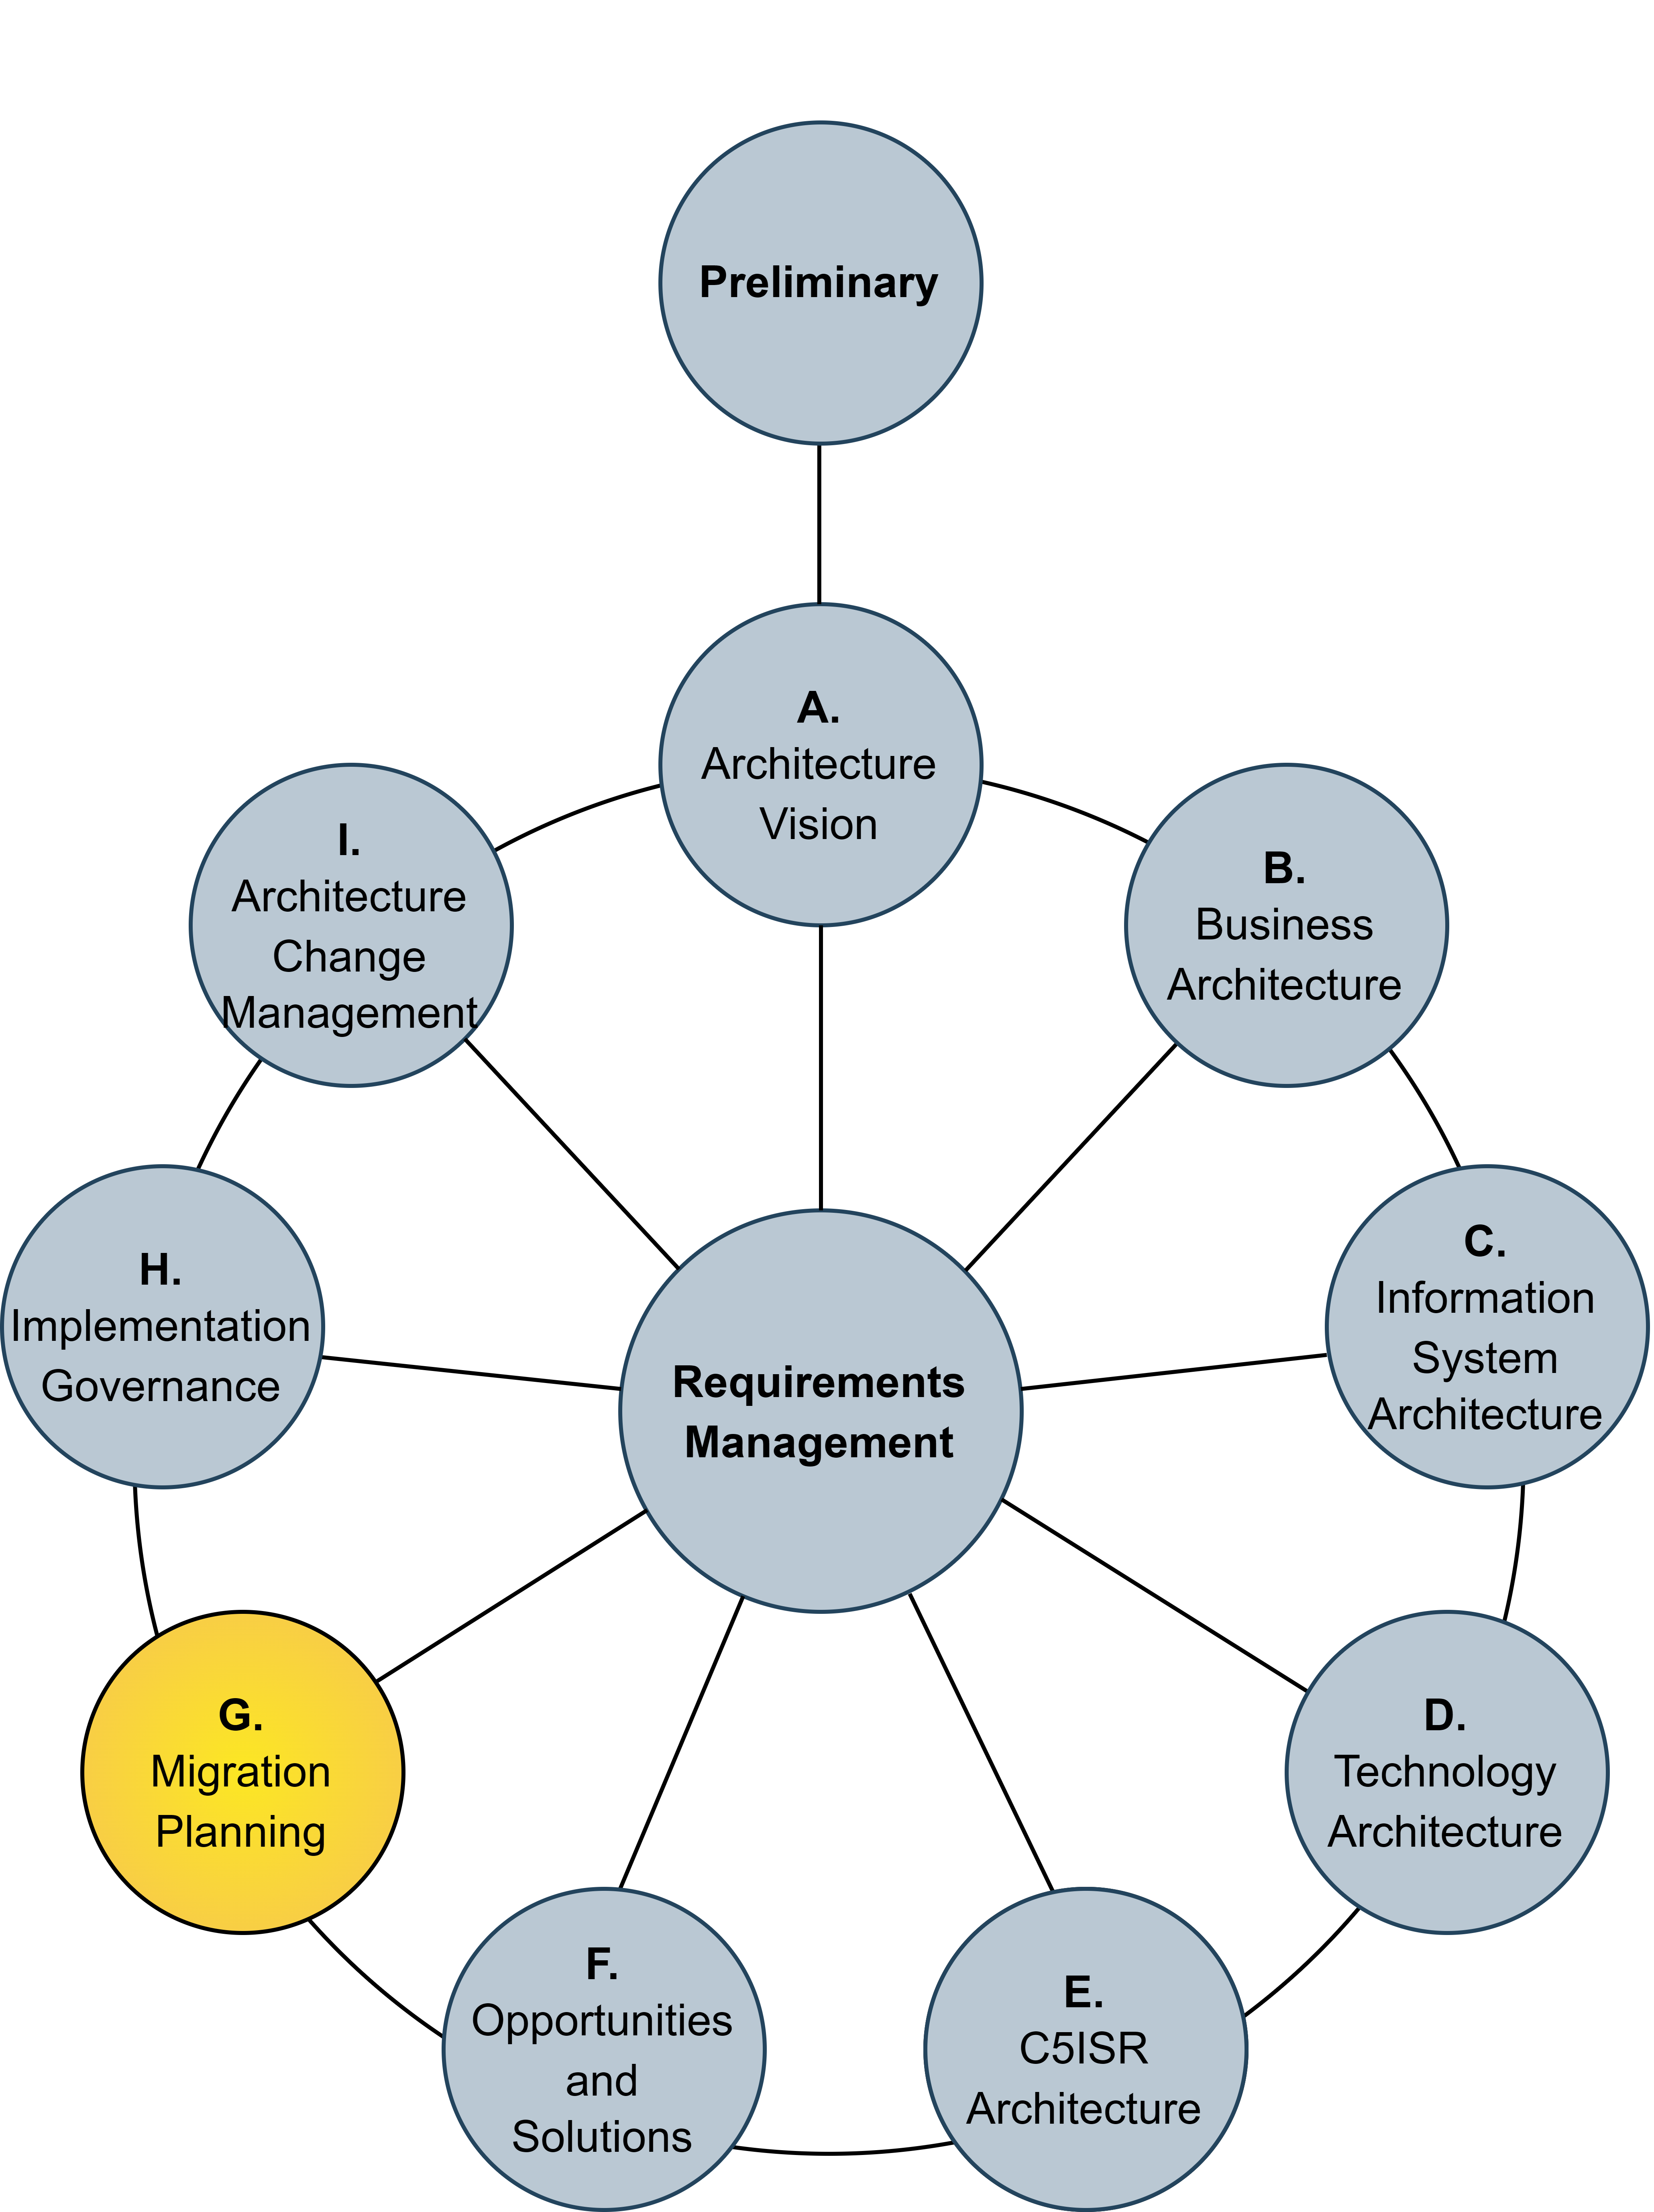
\includegraphics[width=0.42\textwidth]{images/Migration Planning.drawio.png}
\end{figure}

Gambar~\ref{fig:fase-migration} menunjukkan fase \textit{Migration Planning} sebagai kelanjutan langsung dari fase \textit{Opportunities \& Solutions} dalam kelompok realisasi. Posisi berurutan ini memperlihatkan peralihan dari penetapan paket pekerjaan menuju penetapan urutan dan waktu pelaksanaannya. \textit{Input}, \textit{step} dan \textit{output} dapat dilihat pada Tabel~\ref{tab:migration-planning}.

\begin{longtable}{@{}p{0.31\textwidth}p{0.31\textwidth}p{0.31\textwidth}@{}}
\caption{\textit{Input}, \textit{Step}, dan \textit{Output} Fase \textit{Migration Planning}}
\label{tab:migration-planning}\\
\toprule
\textbf{\textit{INPUT}} & \textbf{\textit{STEP}} & \textbf{\textit{OUTPUT}}\\
\midrule
\endfirsthead
\multicolumn{3}{c}{\tablename\ \thetable\ (lanjutan)}\\
\toprule
\textbf{\textit{INPUT}} & \textbf{\textit{STEP}} & \textbf{\textit{OUTPUT}}\\
\midrule
\endhead
\bottomrule
\endfoot
\raggedright
1. \textit{Architecture reference materials}\newline
2. \textit{Request for Architecture Work} dan rencana komunikasi\newline
3. \textit{Statement of Architecture Work}, dokumen \textit{Architecture Vision}, dan \textit{Architecture Repository}\newline
4. Draf \textit{Architecture Definition Document} dan draf \textit{Architecture Requirements Specification}\newline
5. Hasil penilaian kapabilitas\newline
6. \textit{Roadmap} arsitektur dan arsitektur transisi\newline
7. Garis besar rencana implementasi dan migrasi\newline
8. Daftar inisiatif transformasi digital pertahanan
&
\raggedright
1. Mengonfirmasi keterkaitan kerangka manajemen dengan rencana implementasi dan migrasi\newline
2. Menetapkan nilai manfaat setiap paket pekerjaan\newline
3. Memperkirakan kebutuhan sumber daya, waktu pelaksanaan, dan sarana penyampaian\newline
4. Memprioritaskan proyek migrasi melalui analisis biaya-manfaat dan validasi risiko\newline
5. Mengonfirmasi \textit{roadmap} arsitektur dan memutakhirkan \textit{Architecture Definition Document}\newline
6. Menyelesaikan rencana implementasi dan migrasi\newline
7. Menyusun \textit{roadmap} implementasi bertahap jangka pendek, menengah, dan panjang
&
\raggedright
1. Rencana implementasi dan migrasi yang terperinci\newline
2. \textit{Architecture Definition Document} final\newline
3. \textit{Architecture Requirements Specification} final\newline
4. \textit{Roadmap} arsitektur final\newline
5. \textit{Architecture Building Block} yang dapat digunakan ulang\newline
6. \textit{Request for Architecture Work} untuk siklus berikutnya\newline
7. Kontrak arsitektur (\textit{architecture contract})\newline
8. Model tata kelola implementasi\newline
9. \textit{Roadmap} jangka pendek, menengah, dan panjang\arraybackslash\\
\end{longtable}

\textit{Input} fase ini berupa daftar inisiatif dan arsitektur transisi dari fase sebelumnya, yang menjadi bahan mentah bagi penyusunan jadwal pelaksanaan. Kelengkapan daftar inisiatif menentukan ketepatan peta jalan yang dihasilkan, sehingga tidak ada inisiatif penting yang terlewat dari perencanaan.

Langkah-langkah pada fase ini mencakup penilaian manfaat setiap paket pekerjaan, analisis biaya-manfaat dan risiko, penetapan prioritas berdasarkan manfaat dan ketergantungan, serta penyusunan \textit{roadmap} bertahap. Penetapan rentang waktu jangka pendek, menengah, dan panjang menjadi langkah khas fase ini, karena rentang tersebut memungkinkan \textit{roadmap} diselaraskan dengan siklus perencanaan strategis pertahanan dan dengan RPJPN 2025--2045.

\textit{Output} fase ini berupa rencana implementasi dan migrasi yang terperinci beserta \textit{roadmap} jangka pendek, menengah, dan panjang.

\subsubsection{Fase \textit{Implementation Governance}}

Fase \textit{Implementation Governance} memastikan bahwa implementasi inisiatif berjalan sesuai dengan arsitektur yang telah dirancang dan patuh terhadap regulasi nasional serta ketentuan sektor pertahanan.

\begin{figure}[htbp]
\centering
\caption{Kedudukan Fase \textit{Implementation Governance} pada Siklus TOGAF Pertahanan Indonesia}
\label{fig:fase-governance}
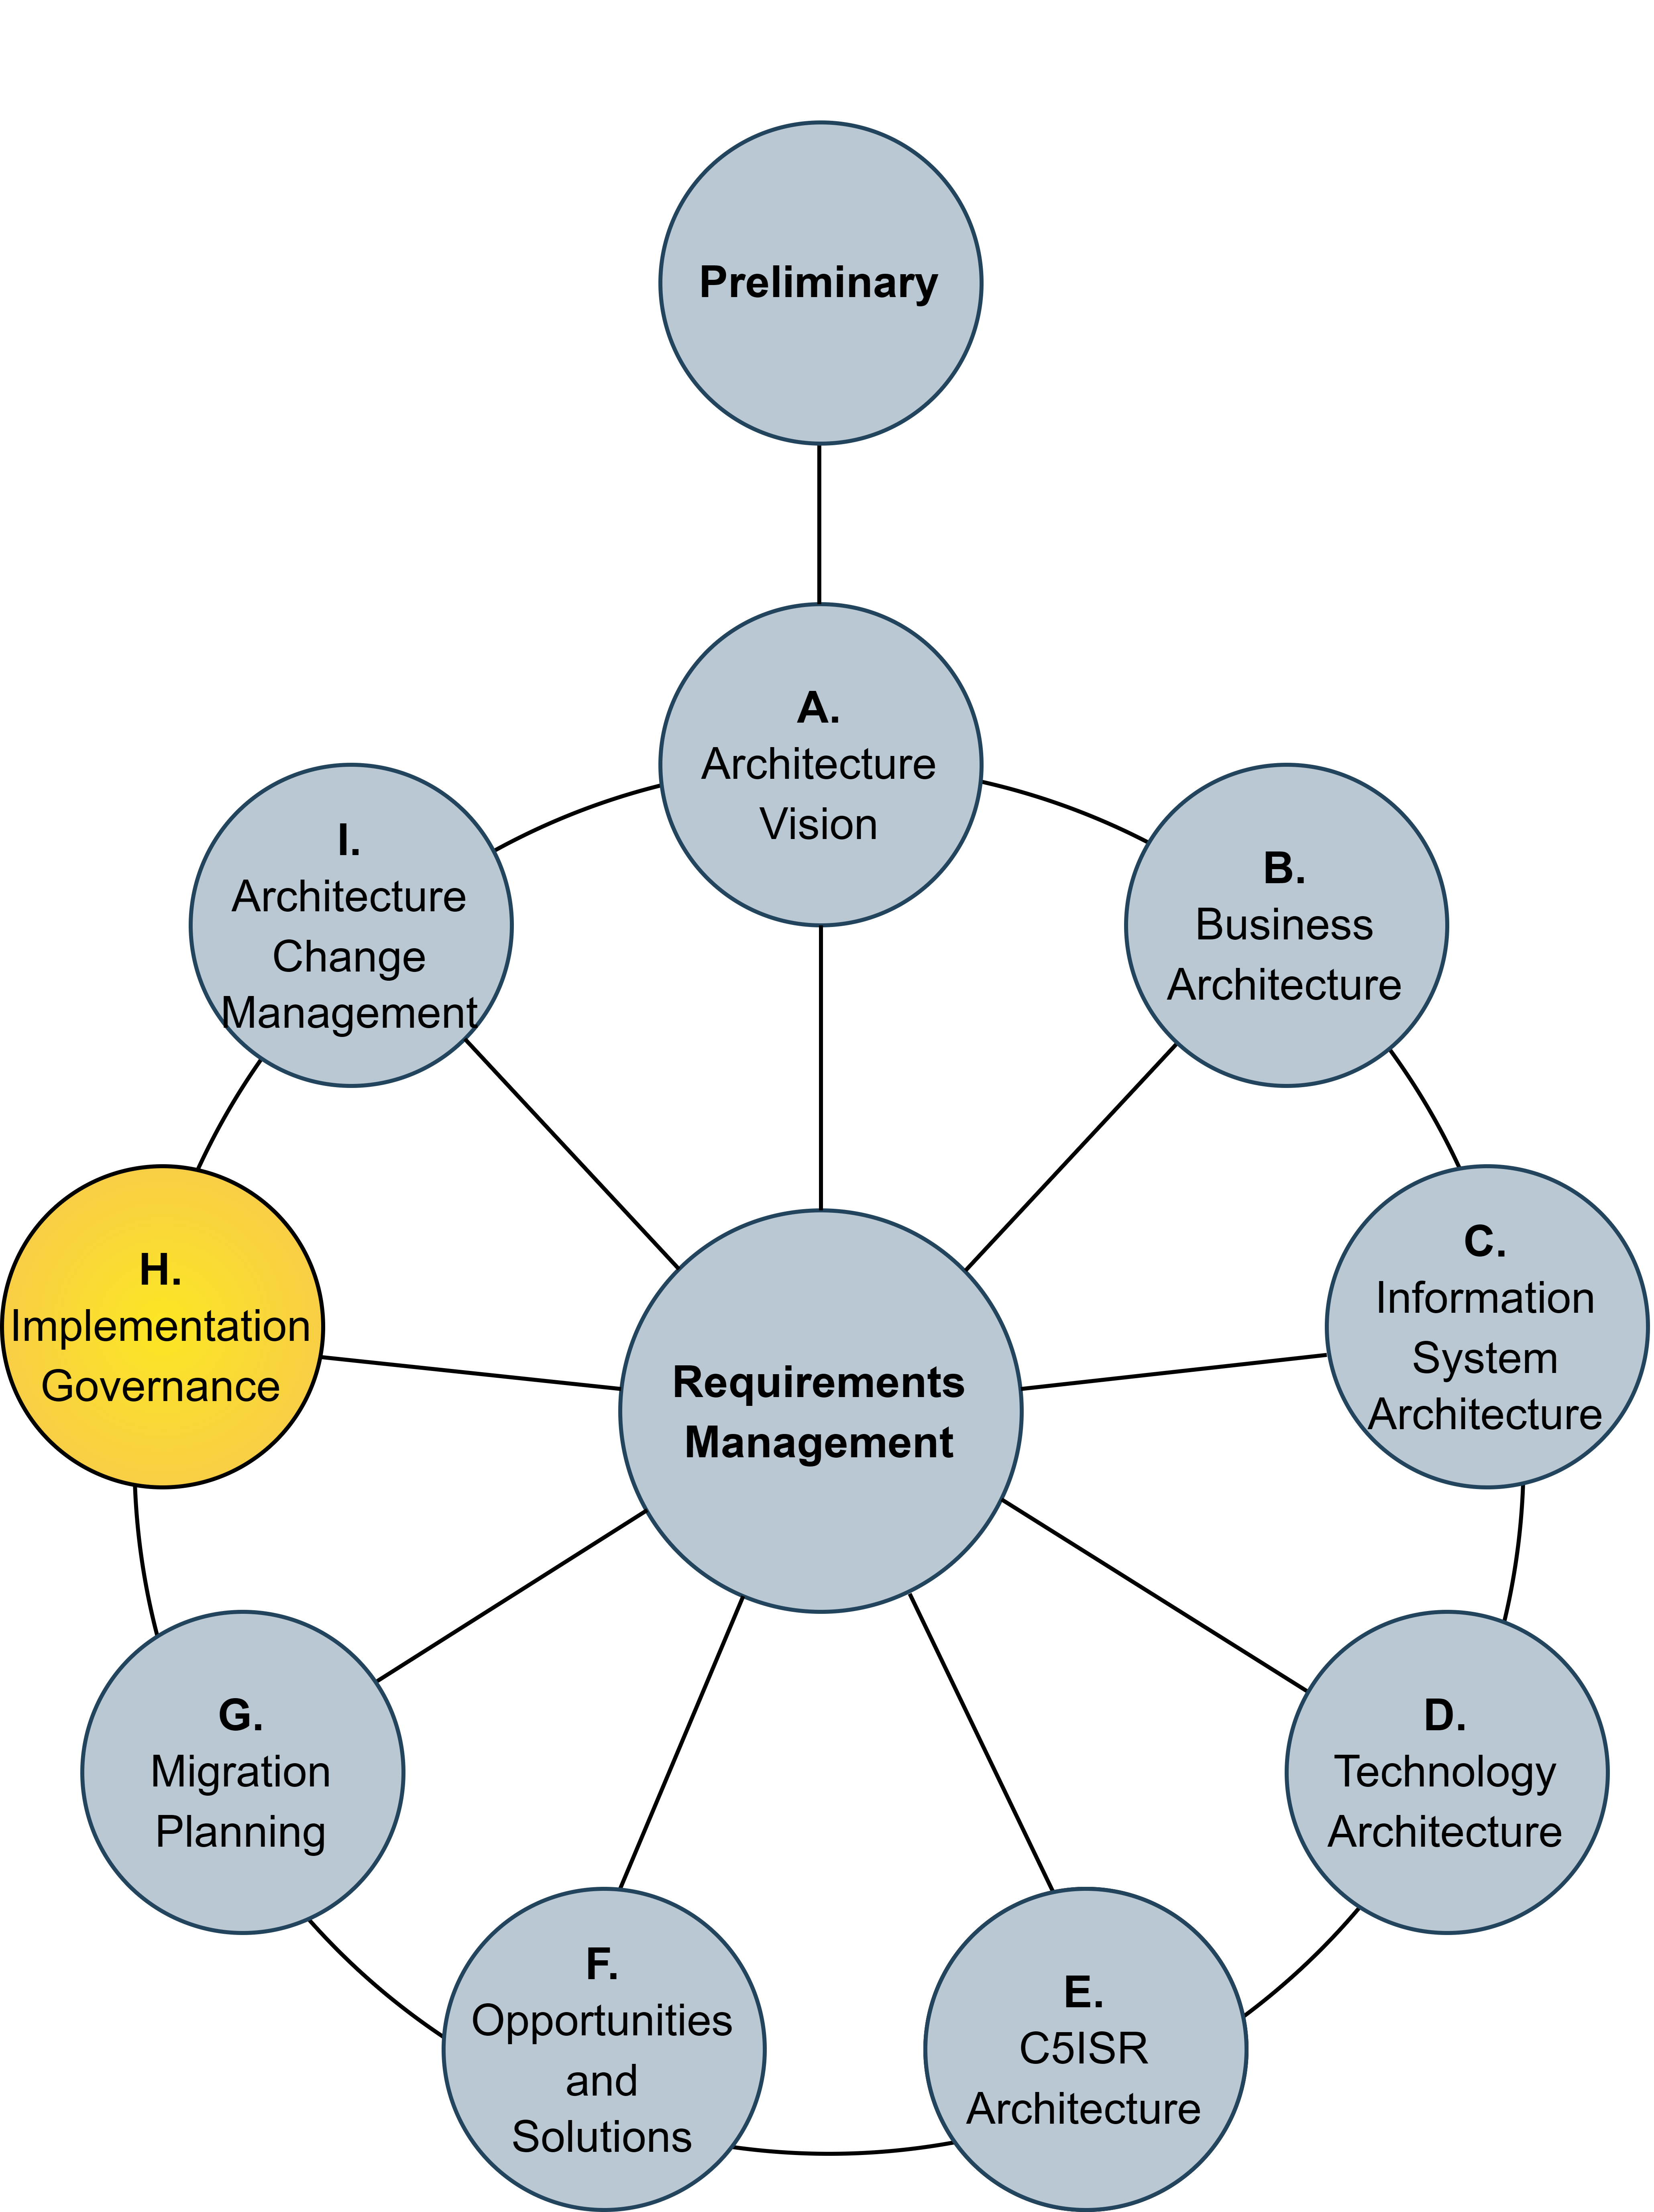
\includegraphics[width=0.42\textwidth]{images/Implementation Governance.drawio.png}
\end{figure}

Gambar~\ref{fig:fase-governance} menempatkan fase \textit{Implementation Governance} setelah fase \textit{Migration Planning}, yaitu pada tahap ketika rencana yang telah disusun mulai diwujudkan menjadi solusi nyata. Posisi ini menegaskan perannya sebagai fase pengendalian pelaksanaan yang menjaga agar solusi yang dibangun tidak menyimpang dari rancangan. \textit{Input}, \textit{step}, dan \textit{output} dapat dilihat pada Tabel~\ref{tab:implementation-governance}.

\begin{longtable}{@{}p{0.31\textwidth}p{0.31\textwidth}p{0.31\textwidth}@{}}
\caption{\textit{Input}, \textit{Step}, dan \textit{Output} Fase \textit{Implementation Governance}}
\label{tab:implementation-governance}\\
\toprule
\textbf{INPUT} & \textbf{STEP} & \textbf{OUTPUT}\\
\midrule
\endfirsthead
\multicolumn{3}{c}{\tablename\ \thetable\ (lanjutan)}\\
\toprule
\textbf{INPUT} & \textbf{STEP} & \textbf{OUTPUT}\\
\midrule
\endhead
\bottomrule
\endfoot
\raggedright
1. \textit{Architecture reference materials}\newline
2. \textit{Request for Architecture Work} dan hasil penilaian kapabilitas\newline
3. Model organisasi untuk arsitektur \textit{enterprise}\newline
4. TOGAF Pertahanan Indonesia\newline
5. \textit{Statement of Architecture Work}, dokumen \textit{Architecture Vision}, dan \textit{Architecture Repository}\newline
6. \textit{Architecture Definition Document} final\newline
7. \textit{Architecture Requirements Specification} final\newline
8. \textit{Roadmap} arsitektur dan arsitektur transisi\newline
9. Model tata kelola implementasi\newline
10. Kontrak arsitektur (standar)\newline
11. Rencana implementasi dan migrasi\newline
12. Prinsip arsitektur pertahanan dan ketentuan regulasi nasional
&
\raggedright
1. Mengonfirmasi ruang lingkup dan prioritas penggelaran bersama manajemen pengembangan\newline
2. Mengidentifikasi sumber daya dan keahlian pelaksana penggelaran\newline
3. Memandu pengembangan solusi dan penggelarannya\newline
4. Melaksanakan tinjauan kepatuhan arsitektur \textit{enterprise}\newline
5. Melaksanakan tinjauan kepatuhan terhadap regulasi nasional dan sektor pertahanan\newline
6. Menetapkan kontrak arsitektur dengan pelaksana implementasi\newline
7. Menjalankan operasi organisasi dan teknologi informasi\newline
8. Melakukan tinjauan pascaimplementasi dan menutup implementasi
&
\raggedright
1. Kontrak arsitektur yang telah ditandatangani\newline
2. Hasil penilaian kepatuhan (\textit{compliance assessments})\newline
3. Permintaan perubahan (\textit{change requests})\newline
4. Solusi terkelola yang patuh terhadap arsitektur\newline
5. Laporan kepatuhan terhadap regulasi nasional dan sektor pertahanan\arraybackslash\\
\end{longtable}

\textit{Input} pada fase ini adalah rencana migrasi, \textit{roadmap} implementasi, serta prinsip arsitektur dan ketentuan regulasi nasional sebagai dasar penilaian kepatuhan.

Langkah-langkah pada fase ini meliputi penetapan kontrak arsitektur dengan pelaksana, pemanduan pengembangan solusi, serta dua jenis tinjauan kepatuhan, yaitu kepatuhan terhadap arsitektur dan kepatuhan terhadap regulasi nasional dan sektor pertahanan.

\textit{Output} fase ini berupa kontrak arsitektur yang telah ditandatangani, hasil penilaian kepatuhan, permintaan perubahan, dan laporan kepatuhan terhadap regulasi. Keluaran tersebut menjadi bukti terkendalinya pelaksanaan sekaligus sebagai sasaran bagi fase \textit{Architecture Change Management} apabila ditemukan kebutuhan penyesuaian arsitektur.

\subsubsection{Fase \textit{Architecture Change Management}}

Fase \textit{Architecture Change Management} bertujuan untuk mengelola perubahan arsitektur secara terkendali sebagai respons terhadap dinamika sektor pertahanan, perkembangan teknologi dan perubahan kebijakan. Fase ini memastikan arsitektur pertahanan tetap relevan dan adaptif melalui pemantauan berkelanjutan serta penilaian dampak perubahan, sehingga siklus \textit{Architecture Development Method} dapat berulang secara berkesinambungan.

\begin{figure}[htbp]
\centering
\caption{Kedudukan Fase \textit{Architecture Change Management} pada Siklus TOGAF Pertahanan Indonesia}
\label{fig:fase-change}
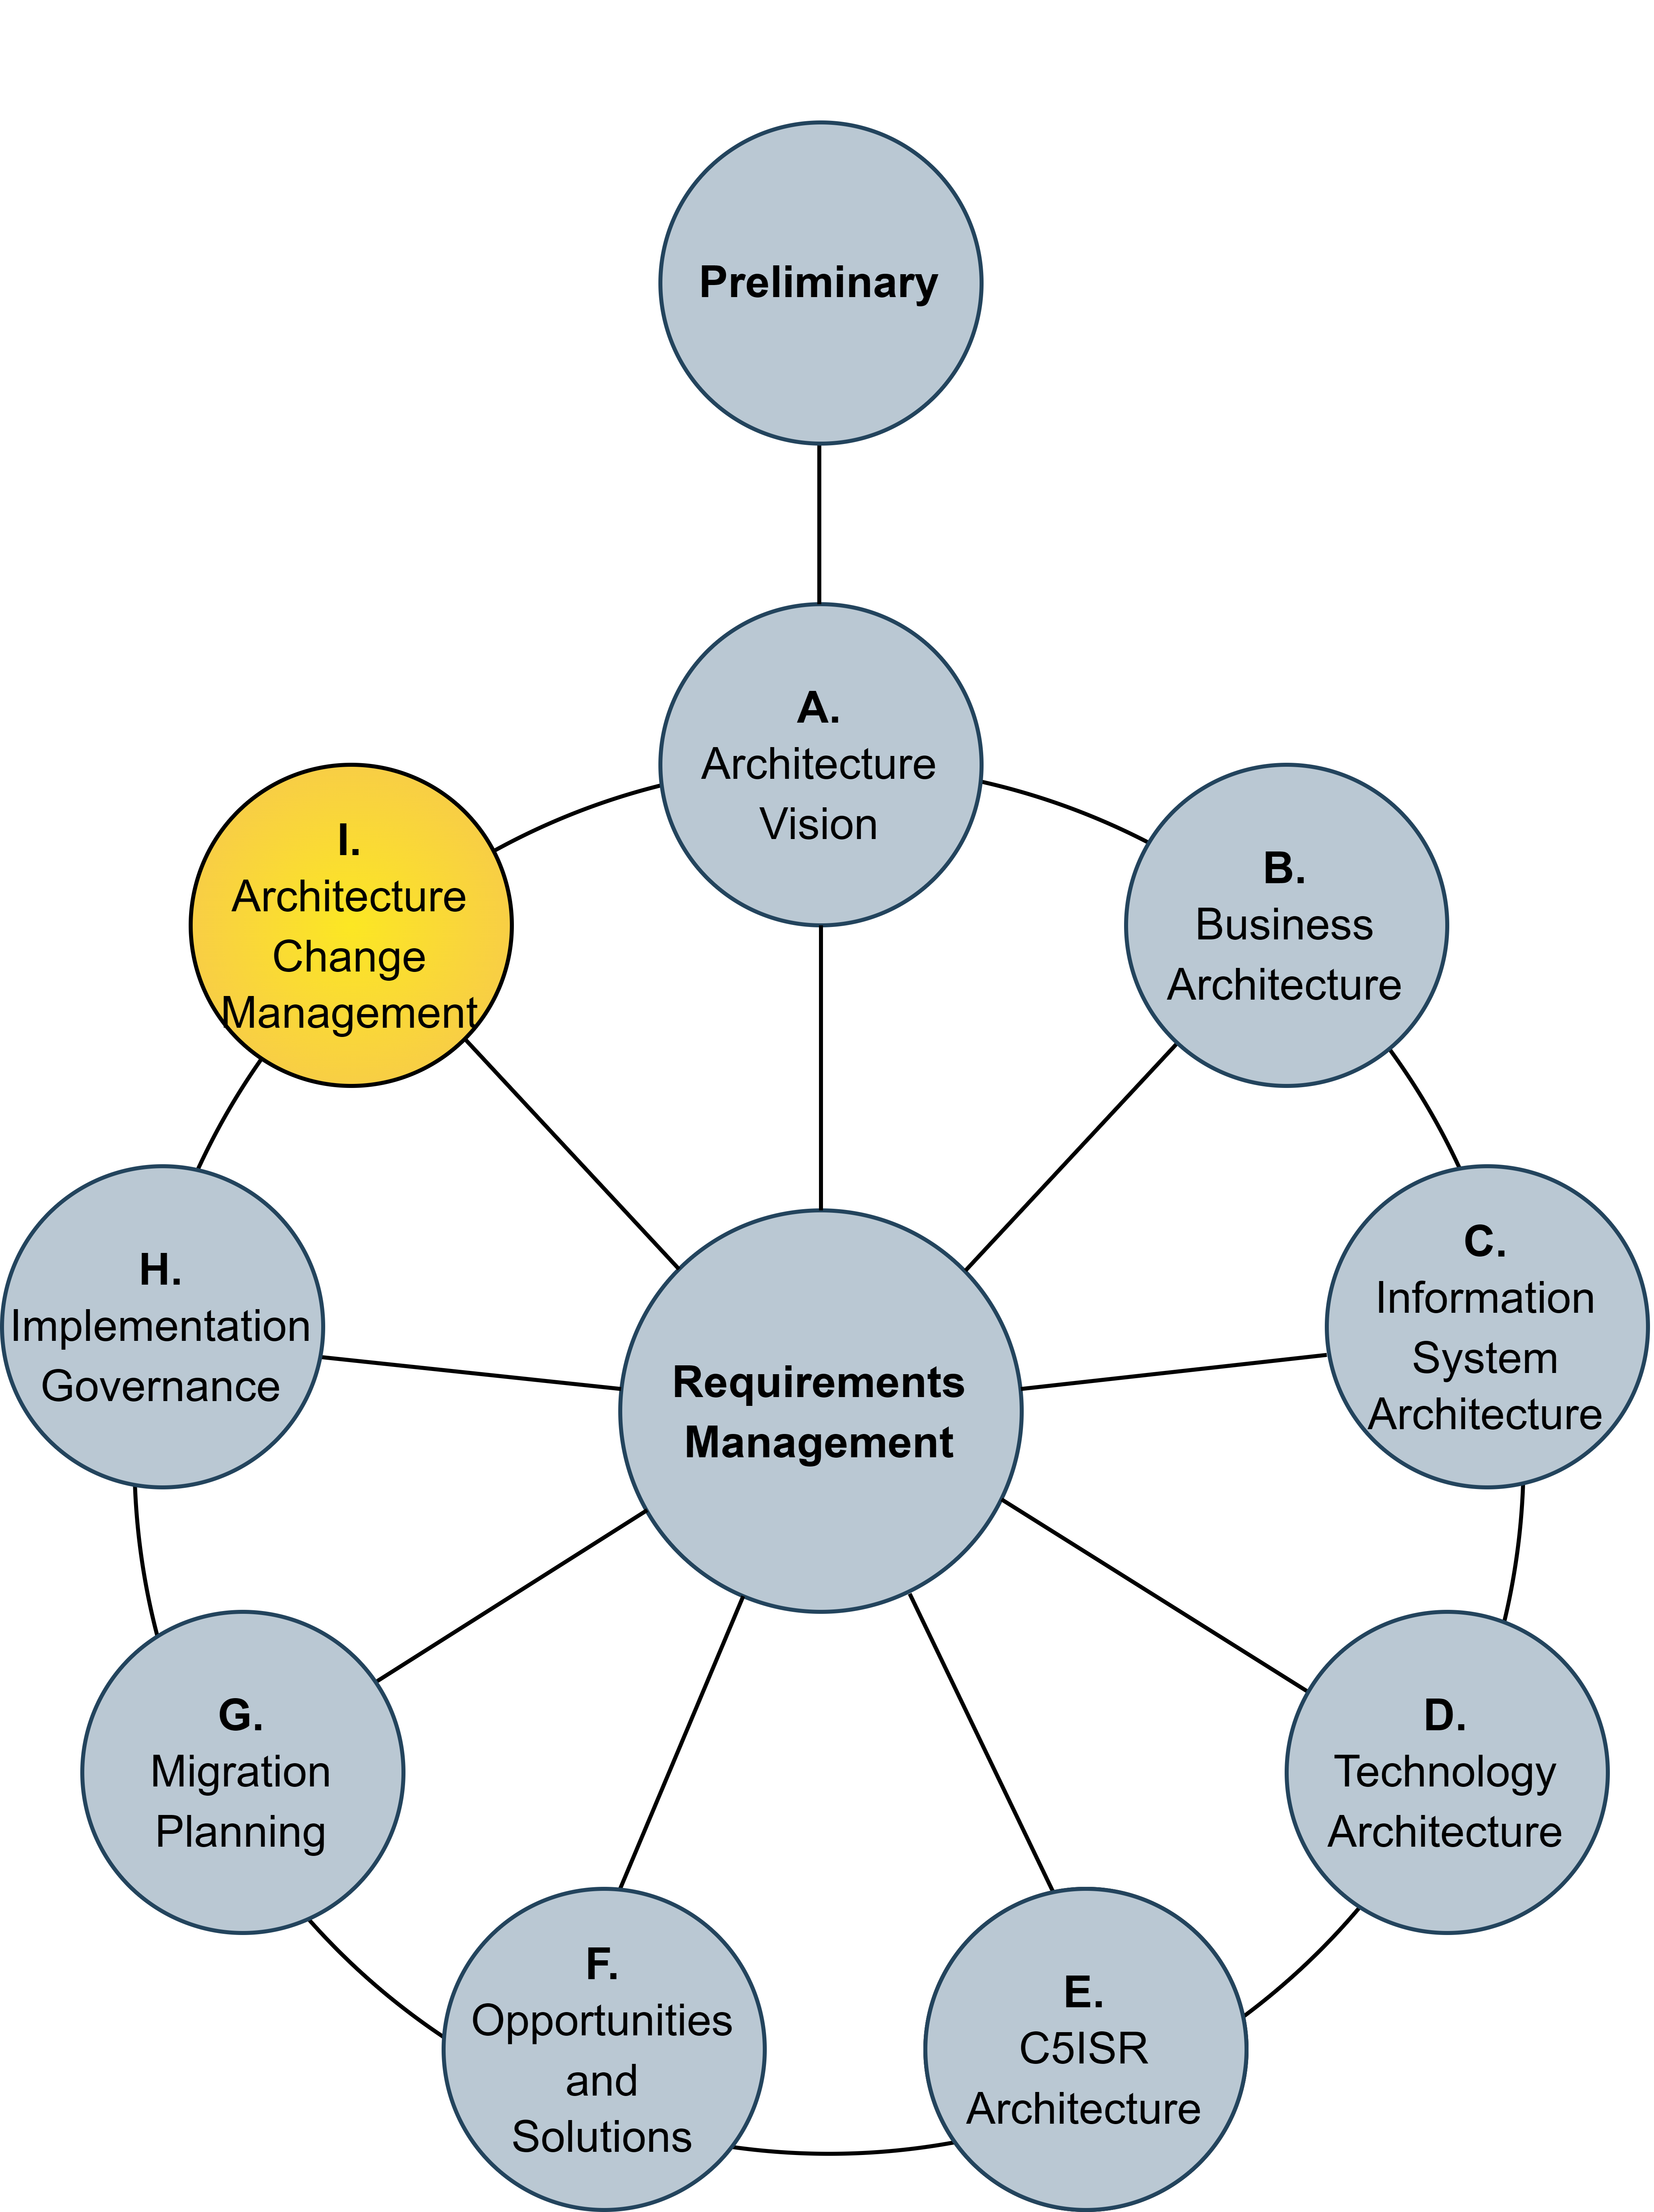
\includegraphics[width=0.42\textwidth]{images/Architecture Change Management.drawio.png}
\end{figure}

Gambar~\ref{fig:fase-change} memperlihatkan TOGAF Pertahanan Indonesia menutup siklusnya dengan fase \textit{Architecture Change Management}, yang terhubung kembali ke fase \textit{Architecture Vision}. Hubungan balik inilah yang menandai sifat berulang keseluruhan siklus, sekaligus menempatkan fase ini sebagai penjaga keberlanjutan yang mengawali siklus baru ketika perubahan menuntut penyesuaian arsitektur. \textit{Input}, \textit{step} dan \textit{output} dapat dilihat pada Tabel~\ref{tab:change-management}.

\begin{longtable}{@{}p{0.31\textwidth}p{0.31\textwidth}p{0.31\textwidth}@{}}
\caption{\textit{Input}, \textit{Step}, dan \textit{Output} Fase \textit{Architecture Change Management}}
\label{tab:change-management}\\
\toprule
\textbf{INPUT} & \textbf{STEP} & \textbf{OUTPUT}\\
\midrule
\endfirsthead
\multicolumn{3}{c}{\tablename\ \thetable\ (lanjutan)}\\
\toprule
\textbf{INPUT} & \textbf{STEP} & \textbf{OUTPUT}\\
\midrule
\endhead
\bottomrule
\endfoot
\raggedright
1. \textit{Architecture reference materials}\newline
2. \textit{Request for Architecture Work}\newline
3. Model organisasi untuk arsitektur \textit{enterprise} dan TOGAF Pertahanan Indonesia\newline
4. \textit{Statement of Architecture Work} dan dokumen \textit{Architecture Vision}\newline
5. \textit{Architecture Definition Document} dan \textit{Architecture Requirements Specification}\newline
6. \textit{Roadmap} arsitektur dan \textit{Architecture Repository}\newline
7. Kontrak arsitektur dan hasil penilaian kepatuhan\newline
8. Rencana implementasi dan migrasi\newline
9. Hasil implementasi dan umpan balik operasional\newline
10. Perubahan lingkungan strategis pertahanan, teknologi, dan regulasi
&
\raggedright
1. Menetapkan proses perwujudan nilai (\textit{value realization process})\newline
2. Menerapkan perangkat pemantauan kinerja arsitektur\newline
3. Mengelola risiko arsitektur\newline
4. Menyediakan analisis bagi manajemen perubahan arsitektur\newline
5. Memantau perubahan lingkungan strategis pertahanan, teknologi, dan regulasi\newline
6. Menilai dampak perubahan terhadap arsitektur\newline
7. Menyusun kebutuhan perubahan untuk memenuhi target kinerja\newline
8. Mengelola proses tata kelola perubahan\newline
9. Mengaktifkan proses pelaksanaan perubahan secara terkendali
&
\raggedright
1. Pemutakhiran arsitektur\newline
2. Perubahan pada \textit{framework} dan prinsip arsitektur\newline
3. \textit{Request for Architecture Work} baru\newline
4. \textit{Statement of Architecture Work} yang dimutakhirkan\newline
5. Kontrak arsitektur yang dimutakhirkan\newline
6. Hasil penilaian kepatuhan yang dimutakhirkan\newline
7. Arsitektur terbarukan dan proses manajemen perubahan\arraybackslash\\
\end{longtable}

\textit{Input} fase ini mencakup hasil implementasi dan umpan balik operasional, serta perubahan lingkungan strategis pertahanan, teknologi, dan regulasi. Kedua kelompok masukan tersebut menjadi pemicu yang menentukan apakah arsitektur perlu disesuaikan, sehingga penyesuaian arsitektur selalu berangkat dari kondisi nyata dan bukan dari asumsi.

Langkah-langkah pada fase ini meliputi pemantauan kinerja arsitektur, pemantauan perubahan lingkungan strategis pertahanan, penilaian dampak perubahan, serta pengelolaan permintaan perubahan secara terkendali. Pemantauan lingkungan strategis pertahanan menjadi langkah khas fase ini, karena perubahan lingkungan ancaman dan kebijakan pertahanan merupakan pemicu perubahan yang bergerak cepat dan berpengaruh besar terhadap kebutuhan arsitektur.

\textit{Output} fase ini berupa pemutakhiran arsitektur, permintaan pekerjaan arsitektur baru, serta perubahan pada kerangka dan prinsip arsitektur bila diperlukan. Keluaran terakhir menegaskan bahwa TOGAF Pertahanan Indonesia bersifat terbuka terhadap penyempurnaan, karena kerangka ini akan terus disesuaikan melalui siklus berikutnya seiring perubahan doktrin, teknologi, dan regulasi.

\section{Evaluasi TOGAF Pertahanan Indonesia}
\label{sec:evaluasi-togaf}

Perlunya dilakukan evaluasi untuk memastikan bahwa kesepuluh kebutuhan yang dirumuskan pada Tabel~\ref{tab:kebutuhan-framework} telah terpenuhi oleh \textit{framework} usulan. Evaluasi ini sekaligus menjawab tingkat pemenuhan yang belum tercapai oleh TOGAF standar pada Tabel~\ref{tab:evaluasi-framework}, yaitu KF-03, KF-04, dan KF-06 yang sebelumnya tidak terpenuhi, serta KF-05 yang sebelumnya baru terpenuhi sebagian.

Hasil evaluasi disajikan pada Tabel~\ref{tab:pemenuhan-togaf}, yang memuat pemenuhan setiap kebutuhan beserta lokasinya.

\begin{longtable}{@{}p{0.07\textwidth}p{0.23\textwidth}p{0.45\textwidth}p{0.15\textwidth}@{}}
\caption{Pemenuhan Kebutuhan \textit{Framework} oleh TOGAF Pertahanan Indonesia}
\label{tab:pemenuhan-togaf}\\
\toprule
\textbf{Kode} & \textbf{Kebutuhan} & \textbf{Mekanisme Pemenuhan} & \textbf{Lokasi pada Bab}\\
\midrule
\endfirsthead
\multicolumn{4}{c}{\tablename\ \thetable\ (lanjutan)}\\
\toprule
\textbf{Kode} & \textbf{Kebutuhan} & \textbf{Mekanisme Pemenuhan} & \textbf{Lokasi pada Bab}\\
\midrule
\endhead
\bottomrule
\endfoot
KF-01 & Metodologi pengembangan preskriptif dan iteratif & Siklus ADM diadopsi secara utuh sebagai basis \textit{framework}, dengan \textit{Requirements Management} tetap berada di pusat siklus. & III.2.3\\
\addlinespace
KF-02 & Cakupan domain arsitektur inti & Fase \textit{Business Architecture}, \textit{Information Systems Architecture}, dan \textit{Technology Architecture} dipertahankan tanpa pengurangan. & III.2.3.3; III.2.3.4; III.2.3.5\\
\addlinespace
KF-03 & Akomodasi domain C5ISR & Penambahan Fase E \textit{C5ISR Architecture} sebagai domain arsitektur tersendiri, diperkuat prinsip \textit{Integrated Command \& Control}. & III.2.1; III.2.2; III.2.3.6\\
\addlinespace
KF-04 & Keamanan siber sebagai prinsip perancangan & Penetapan prinsip \textit{Security by Design} yang mengikat seluruh fase, dengan perancangan fondasi keamanan siber terpadu pada Fase D dan Fase E. & III.2.2; III.2.3.5; III.2.3.6\\
\addlinespace
KF-05 & Dukungan interoperabilitas lintas entitas & Penetapan prinsip \textit{Interoperabilitas} disertai penetapan standar integrasi lintas matra pada arsitektur data, aplikasi, dan C5ISR. & III.2.2; III.2.3.4; III.2.3.6\\
\addlinespace
KF-06 & Keterkaitan dengan doktrin dan strategi pertahanan & Doktrin dan strategi pertahanan nasional ditetapkan sebagai \textit{input} Fase \textit{Preliminary} dan \textit{Architecture Vision}, diperkuat prinsip \textit{Smart Defence Oriented}. & III.2.2; III.2.3.1; III.2.3.2\\
\addlinespace
KF-07 & Keselarasan dengan regulasi nasional & Kerangka regulasi nasional ditetapkan sebagai \textit{input} Fase \textit{Preliminary}, diperkuat prinsip \textit{Governance \& Compliance}. & III.2.2; III.2.3.1\\
\addlinespace
KF-08 & Fleksibilitas dan kemampuan kustomisasi & Penyesuaian dibatasi pada satu penambahan fase yang bersifat aditif (\textit{minimal necessary modification}), sehingga sifat \textit{tailorable} ADM tetap terjaga. & III.2.1\\
\addlinespace
KF-09 & Tata kelola arsitektur dan manajemen perubahan & Fase \textit{Implementation Governance} dan \textit{Architecture Change Management} dipertahankan, dengan \textit{output} berupa kerangka tata kelola arsitektur pada Fase \textit{Preliminary}. & III.2.3.1; III.2.3.9; III.2.3.10\\
\addlinespace
KF-10 & Ketersediaan dan kematangan ekosistem & TOGAF digunakan sebagai basis penyesuaian sehingga ekosistem pengetahuan dan ketersediaan terbukanya tetap dapat dimanfaatkan. & III.2.1\\
\end{longtable}